\documentclass{wileySix}
\usepackage{w-bookps}


\usepackage{graphicx}
\usepackage{enumitem}

\setcounter{secnumdepth}{3}

\setcounter{tocdepth}{2}

\begin{document}

\booktitle{Web Service}
\subtitle{Semua Tentang Komunikasi antar Aplikasi Berbasis Protokol internet}

\author{Rolly Maulana Awangga}

\halftitlepage
\titlepage

\offprintinfo{Web Service, pre-release}{Rolly Maulana Awangga}


\begin{copyrightpage}{2018}
Web Service / Rolly Maulana Awangga
\end{copyrightpage}


\dedication{For my family}

\contentsinbrief %optional
\tableofcontents
\listoffigures %optional
\listoftables  %optional

%%%%%%%%%
%%Content 
%%%%%%%%%

\part[Pengenalan Web Service]
{Pengenalan\\ Web Service}

\chapter[Contoh]
{Contoh\\ Latex}
tugas 1 :
Tuliskan resume atau tutorial;

2A :
1. Python instalasi dan definisi dan contoh kode awal
2. wsgi definisi dan contoh contoh
3. cgi definisi dan contoh
4. uwsgi instalasi definisi dan contoh
5. Install the Windows Subsystem for Linux


2B :
1. contoh aplikasi web service
2. pengertian web service
3. protokol
4. port
5. penggunaan aplikasi testing web service


2C :
1. internet
2. web
3. backend
4. frontend

Syarat :
1. gunakan SPOK yang benar
2. Tanda baca yang benar
3. Penggunaan Huruf kapital yang benar

buat grup kelompok di github dan fork webservice

Parameter(baca standar penulisan latex) :
1. itemize dan enumerate yang benar (10)
2. gambar dan referensi disebutkan dalam kalimat dengan benar (10)
3. penggunaan section subsection subsubsection yang benar (10)
4. Penggunaan tabel atau verbatim atau equation (10)
5. commit sehari(min 50 kata) per anggota kelompok selama 6 hari (60)

Nilai akhir X persentasi plagiarisme = Nilai tugas

(GUnakan standar penggunaan git)
jika ada error maka minus 5 setiap kali pull request

\chapter[RESTful]
{Definisi\\ RESTful}
\begin{itemize}
\item Ahmad Syafrizal Huda (1164062)
\item Annisa Fathoroni (1164067)
\item Puad Hamdani (1164084)
\item Rahmi Roza (1164085)
\item Tasya Wiendhyra (1164086)
\end{itemize}

\section{Definisi RESTful Web Service}
REST merupakan salah satu macam web service yang memasukkan konsep perpindahan antar state. State disini bisa dibayangkan seperti jika browser meminta suatu halaman web, maka server akan mengirimkan state halaman web yang sekarang ke browser. Menurut salah satu perkembangan Tidwell, D., 2001 bernavigasi melalui link-link yang disediakan sama halnya dengan mengganti state dari halaman web. Begitu pula REST bekerja, dengan bernavigasi melalui link-link HTTP untuk melakukan aktivitas tertentu, seakan-akan terjadi perpindahan state satu sama lain \cite{indrawan2017implementasi}.
Pada gambar \ref{labelgambar} menerangkan cara Rest Web Service melakukan request kepada server kemudian server membalasnya dengan result berupa json. Metode tersebut telah dikembangkan oleh Roy Thomas Fielding dalam disertasinya tentang Architectural Style.  Dalam disertasinya tersebut REST (Representational state transfer) didefinisikan sebagai suatu gaya arsitektur perangkat lunak untuk pendistribusian sistem hypermedia seperti WWW \cite{rofiq2017implementasi}.
\begin{figure}[ht]
\centerline{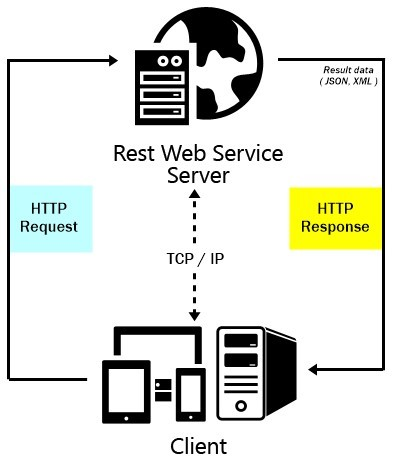
\includegraphics[width=1\textwidth]{figures/1restful.JPG}}
\caption{RESTful}
\label{labelgambar}
\end{figure}

\section{Prinsip atau Karakter Pada RESTful}
RESTful adalah salah satu teknologi web service untuk membuat suatu sistem yang terdistribusi dimana cara kerjanya berdasarkan resource. RESTful sendiri merupakan software yang didesain untuk penekanan pada skalabilitas,kesederhanaan dan kegunaan. Metode dalam REST terdiri dari empat prinsip utama teknologi, yaitu \cite{aji2016penerapan}:
\begin{enumerate}
\item Resource identifier melalui Uniform Resource Identifier (URI), REST Web service mencari sekumpulan sumber daya yang mengidentifikasi interaksi antar klien.
\item Uniform interface, sumber daya yang dimanipulasi CRUD (Create, Read, Update, Delete) menggunakan operasi PUT, GET, POST, dan DELETE.
\item Self-descriptive messages, sumberdaya informasi tidak terikat, sehingga dapat mengakses berbagai format konten (HTML, XML, PDF, JPEG, Plain Text dan lainnya). Metadata pun dapat digunakan.
\item Stateful interactions melalui hyperlinks, setiap interaksi dengan suatu sumber daya bersifat stateless, yaitu request messages tergantung jenis kontennya.
\end{enumerate}

\section{Sejarah RESTful}
REST tidak menarik perhatian banyak ketika pertama kali diperkenalkan pada tahun 2000 oleh Roy Fielding di Universitas California, Irvine, dalam disertasinya akademik, Architectural gaya dan arsitektur perangkat lunak berbasis desain jaringan, yang menganalisa set dari prinsip-prinsip arsitektur perangkat lunak yang menggunakan Web sebagai platform untuk komputasi terdistribusi (Lihat sumber daya untuk link ke disertasi ini). Sekarang, tahun setelah diperkenalkan, utama kerangka untuk REST telah mulai muncul dan masih sedang dikembangkan karena itu dijadwalkan, misalnya, akan menjadi bagian integral dari Java 6 melalui JSR-311 \cite{rodriguez2008restful}.

\section{Contoh-Contoh Penerapan  RESTful}
\subsection{Implementasi RESTful Web Service untuk Sistem Penghitungan Suara Secara Cepat pada Pilkada}
Metode ini yang digunakan oleh penyelenggara pemilihan umum untuk menentukan hasil pilkada. Dengan memanfaatkan teknologi yang ada, proses pengumpulan data hasil perolehan suara bisa dilakukan dengan lebih cepat. Salah satu metode baru yang bisa digunakan untuk melakukan proses tersebut adalah metode perhitungan cepat riil. Metode ini memanfaatkan teknologi informasi dan komunikasi untuk melakukan proses penghitungan suara. Real-quick count mengambil hasil perhitungan dari semua tempat pemungutan suara (TPS). Tetapi hasil tersebut dikirim langsung dari TPS ke lembaga penyedia informasi hasil perhitungan cepat, tidak melalui prosedur seperti pada real count yang mengharuskan pengumpulan data berjenjang, oleh karena itu waktu yang dibutuhkan untuk memperoleh semua hasil suara bisa dioptimalkan. Pada jurnal ini dilakukan perbandingan antara SOAP dan REST pada aplikasi mobile dan multimedia conference. Hasil penelitian yang dilakukan pada aplikasi mobile computing menunjukkan bahwa ukuran pesan pada RESTful web service mencapai 9 sampai 10 kali lebih kecil dibandingkan ukuran pesan dari web service berbasis SOAP \cite{rofiq2017implementasi}.

\subsection{Implementasi RESTful untuk Sales Order dan Sales Tracking Berbasis Mobile}
Bagian penjualan merupakan bagian yang paling penting dalam penjualan produk. Perusahaan membutuhkan sistem yang dapat membantu aktivitas dan pemesanan produk. dengan membuat sebuah Controller terlebih dahulu,yang berperan untuk menentukan informasi apa yang akan disampaikan pada saat client mengakses web service. Dibuat dengan arsitektur REST dengan menggunakan method yang di dukung protokol HTTP seperi method DELETE, UPDATE, CREATE,dll. Aplikasi mobile ini akan menggunakan data dari GPS untuk memastikan lokasi penjual juga dilengkapi barcode untuk mempercepat input data barang \cite{kurniawan2015implementasi}.

\subsection{Implementasi REST Web Service Pada Aplikasi Pengolah Pesan Yahoo Messenger Pada CV. Meliana Pratama}
Mengimplementasikan REST Web Service pada aplikasi pengolah pesan Yahoo Messenger (YM). Aplikasi REST Web Service dapat dijadikan sebagai miidleware antara aplikasi pengolahan pesan Yahoo Messenger (YM) dengan database, sehingga proses transaksi ke database menjadil lebih efisien. Hal ini dikarenakan aplikasi client tidak perlu mengetahui database apa yang digunakan oleh server \cite{ikrom2015implementasi}.

\subsection{Implementasi RESTful Web Service Pada Aplikasi Iklan Baris Online}
Pada implementasi aplikasi ini menerapkan restful web service yang dimana server akan berinteraksi dengan client pada interface yang sama atau seragam. Server akan meng-host resource sedangakn client akan menjadi konsumen dari resource yang disediakan server. Pada saat server meminta atau request data script request akan dikirim dari client ke server berbentuk alamat url yang kemudian memanggil file PHP yang mengakses data dari databse server. saat pengambilan data, client akan memanfaatkan API yang terdapat dalam server. Setelah mendapat data dari client, server kemudian akan menyebar informasi yang dibutuhkan berupa kebutuhan barang/jasa yang bersangkutan kepada member atau client \cite{fauziah2014aplikasi}.

\subsection{Implementasi Protokol OAuth 1.0 Sebagai Autentikasi pada Aplikasi SMS Blast Berbasis Android}
Sebuah aplikasi SMS Blast berbasis Android dan sebuah web service yang digunakan oleh aplikasi untuk melakukan request terhadap data nomor telepon terhadap data yang sudah ada. OAuth menggunakan token pada setiap request. Web service akan membangkitkan token yang berbeda pada setiap request dari consumer. Penggunaan token ini dapat meminimalkan kemungkinan terjadinya serangan Man in the Middle Attack dan Hijacking Attack
\cite{saputra2017implementasi}

\subsection{Implementasi RESTful Web Service One Chip Multi-Client Untuk Mengoptimalkan Penjualan Pulsa All Operator}
One  Chip  All  Operator adalah sebuah chip untuk pengisian pulsa kesemua operator selluler GSM dan CDMA bahkan juga dapat digunakan untuk pengisian pulsa listrik atau listrik prabayar. Chip atau kartu perdana  yang  digunakan bukan kartu Khusus atau tidak harus dipesan kedealer penyedia pelayanan pengisian pulsa,Chip yang   digunakan cukup perdana biasa,jadi nomor  yang dipakai sehari-hari dapat dijadikan sebagai chip untuk pengIsian pulsa ke semua operator. Proses awal yang dilakuakanya itu peses deployment restful  web  service. Deployment  restful web service  merupakan proses menjalankan web service pada server seperti apache tomcat agar aplikasi client dapat mengakses service database\cite{indrawan2017implementasi}.

\subsection{Implementasi Protocol Buffers pada Aplikasi Weblog Client dan Server}
Web service yang digunakan untuk mengirimkan dan menerima   protobuf  messages adalah  RESTful  web service  yang  merupakan  teknologi  web  service  yang ringan dan mudah diimplementasikan. Client mengirimkan data yang telah diserialisasikan dalam bentuk protobuf message melalui  HTTP  request kepada RESTful  service pada server. Protobuf  message kemudian diubah menjadi data semula dengan program deserialisasi yang telah ada di server \cite{wibowo2011implementasi}.

\subsection{Implementasi Restful Web Service Menggunakan AsyncTask pada Aplikasi Library Automation Berbasis Android}
Dengan menggunakan aplikasi Library automation berbasis android ini diharapkan dapat mempermudah untuk mengakses informasi terkait referensi yang terdapat pada perpustakaan fisik penggunaan RESTful web service dengam menggunakan AsyncTask sebagai prosesnya juga dinilai cukup baik dari segi penggunaan. Diharapkan untuk pengembangan selanjutnya meningkatkan akurasi pencarian supaya end user tidak merasa bingung saat mencari informasi \cite{yudhistiraimplementasi}.

\subsection{Penerepan Restful pada Aplikasi Ayo Piknik Indonesis Berbasis Android}
Aplikasi Ayo Piknik Indonesia berbasis android yang berbasis dengan Web-server menggunakan metode Restful Webservice yang bisa menampilkan informasi wisata dengan cepat dan tepat serta pengguna juga dapat memberikan usulan tempat wisata yang baru. Kemudian akan dilakukan verifikasi agar bisa ditampilkan. Selain itu aplikasi ini juga  dapat menambahkan data wisata dengan google maps untuk memudahkan wisatawan ataupun penduduk lokal \cite{aji2016penerapan}.

\section{Pengembangan Sistem Informasi RESTful Web Service}
Pengembangan sistem informasi kependudukan berbasis mobile dan restful pada web service yaitu\cite{kurniawati2016pengembangan}:
\begin{enumerate}
\item REST Web Service pada tahap ini akan dibuat web service yang diletakkan pada server pusat untuk mengolah data JSON. Web service memiliki 3 method yaitu json decode yaitu untuk parsing data masukan, StoreData dan json encode parsing untuk data keluaran. Parameter masukan dari database SQLite ke MySQL tampak pada gambar 5, akan diparsing ke dalam format Array. StoreData yang berhubungan langsung dengan database dalam proses input, status gagal atau sukses akan disimpan dalam Array dan diolah lagi menjadi format JSON sebagai keluaran dari web service.
\item Aplikasi Android Antarmuka aplikasi android saat dijalankan akan muncul form login. Pengguna aplikasi yaitu kepala lingkungan memasukkan username dan password kemudian tekan tombol login
\end{enumerate}

\subsection{Pengembangan Sistem Informasi Kependudukan Berbasis Moblie Dan RESTFful Web Service}
Sensus biasa dilakukan secara manual, yaitu door-to-door ke setiap rumah warga namun hal tersebut membutuhkan waktu yang lama dan tidak cukup efektif, lalu dibuat solusi dari permasalahan tersebut dengan mengintegrasikan RESTful web service pada perangkat Android. Diimplementasikan pada Android karena Android memiliki kelebihan dapat mengakses database secara offline yaitu SQLite sehingga lokasi yang berada di pedalaman tetap dapat terinputkan ke database meski tidak ada jaringan internet.
Cara kerjanya yaitu petugas sensus akan memasukan data di perangkat android, yang kemudian datanya akan dimasukkan kedalam database. Webservice RESTful ini berfungsi sebagai komunikator antara android dengan database pusat. Web service ini diletakkan di server pusat untuk mengolah data JSON. Parameter masukkan dari SQLite ke MySQL akan di parsing ke format array yang diubah lagi menjadi JSON sebagai hasil dari web servicenya \cite{kurniawati2016pengembangan}.

\section{Kelebihan dan Kekurangan RESTful Web Service}
Pada tabel \ref{table:contoh} merupakan kelebihan dan kekurangan daripada RESTful Web Service dimana RESTful Web Service ini sangat berguna dalam implementasinya \cite{nugroho2012perbandingan}.
\begin{table}[h]
\begin{tabular}{|c|c|c|}
\hline
Jenis Web Service&Kelebihan&Kekurangan\\
\hline
RESTful Webs Service&-Implementasi RESTful Web Service relatif& -Struktur data yang sangat kompleks\\
&sederhana dalam hal pemrogramannya karena& sukar diadaptasi ke dalam URL.\\
&menggunakan standar-standar yang telah&\\
&diterima secara luas (HTTP, XML, dan URL).&\\
&-Server dan klien HTTP dikenali&-Implementasi dan kinerjanya sangat bergantung\\
&oleh sebagian besar bahasa pemrograman&pada kapasitas jaringan yang digunakan\\
&dan hampir semua platform perangkat&\\
&keras/perangkat lunak yang saat ini populer.&\\
\hline
\end{tabular}
\label{table:contoh}
\end{table}

\section{Implementasi PHP Web Service Sebagai Penyedia Data Aplikasi Mobile}
Dapat disimpulkan bahwa PHP Web Service bisa diimplementasikan dalam aplikasi mobile yang membutuhkan data dinamis. Pengujian atas web service bisa dilakukan dengan membuat file PHP secara manual ataupun menggunakan SOAP web service. Untuk memudahkan pemanggilan data bisa dilakukan modifikasi dengan memberikan layer tambahan berupa PHP File yang memanggil pada SOAP web service
\cite{surendra2014implementasi}.


%\chapter[Web]
%{Definisi\\ Web}
%%\begin{itemize}
%\item Imron Sumadireja (1164076)
%\item Jesron Marudut (1164077)
%\item Lusia Violita Aprilian (1164080)
%\item Mhd. Zulfikar Akram Nst. (1164081)
%\end{itemize}

\section{Pengertian Website}
World wide web (www atau web) merupakan halaman situs informasi yang dapat diakses secara cepat atau sarana
antar muka informasi di internet. Web dapat menggabungkan teks, grafik, dan multimedia. Web memudahkan
penggunanya untuk mengakses informasi melalui konsep hypertext sehingga memungkinkan  suatu text untuk
menjadi acuan membuka dokumen laindo. Informasi dapat mudah disebar dan diakses.

\subsection{Sejarah Website}
Sementara itu World wide web (www) dikembangkan pertama kali oleh Tim Berners-Lee pada tahun 1989. Pada
awalnya, Tim mengusulkan WWW sebagai suatu cara berbagai dokumen diantara para peneliti. Dokumen online dapat
diakses melalui alamat unik yang disebut Universal Resource Locator atau URL. Selain itu WWW tidak hanya
dikembangkan untuk keperluan para peneliti, namun juga dikembangkan untuk kalangan pendidikan, bisnis dan
perorangan. Berdasarkan penjelasan singkat diatas dapat disimpulkan bahwa antara web dan internet memiliki
hubungan yang sangat erat walaupun keduangnay tidak bisa dikatakan sama. Web merupakan bagian dari layanan
yang dapat berjala di atas teknologi internet.

\subsection{Jenis-jenis website}
Website dikelompokan dalam beberapa jenis-jenis Website agar dapat memudahkan dalam menentukan jenis website
yang akan ditentukan. Dan berikut jenis-jenis website yang dikelompokan atas beberapa dasar:
\begin{enumerate}
\item Jenis Website berdasarkan sifat;
\begin{itemize}
\item Website Statis, merupakan web yang kontenya hampir jarang diubah
\item Website Dinamis, Web yang konten atau isinya dapat berubah-ubah setiap saat
\end{itemize}
\item Jenis Website yang dikelompokkan berdasarkan Bahasa Pemrogramannya;
\begin{itemize}
\item Server side, Website yang memakai bahasa pemrograman yang tergantung dengan servernya
\item Client side, adalah web yang tidak perluu server untuk menjalankannya. Cukup diakses dengan browser.
\end{itemize}
\item Jenis-jenis Web menurut tujuannya;
\begin{itemize}
\item Web personal, biasanya web ini merupakan web yang berisi informasi seorang
\item Corporate Web, website yang dimiliki sebuah institusi atau perusahaan.
\item Web Portal, Web ini berisi banyak layanan, seperti berita, email dan jasa
\item Web Forum, sebuah web yang dibuat sebagai sarana diskusi.
\end{itemize}
\end{enumerate}
	
\subsection{Keuntungan Web}
Keuntungan penggunaan web diantaranya yaitu :
\begin{itemize}
\item Informasi dapat diberikan segera(tepat waktu) dan diperbarui secara berkala.
\item Presentasi fleksible dan visibilitas dapat menyediakan ragam isyarat untuk diseminasi informasi.
\item Informasi dapat diorganisir melalui tautan dan menu, berbagai tingkatan informasi dapat disediakan format file yang berbeda dapat digunakan untukj informasi yang dapat diunduh. Integrasi informasi dapat dilakukann melalui tautan dan seksi lain, halaman lain, atau web lain.
\item Tauta  dan menu dapat menyediakan informasi bagi pemangku kepentingan yang berbeda, informasi dapat pula diberikan melalui daftar email kepada pemangku kepentingan.
\item Setiap orang yang dapat mengakses web dapat memperoleh informasi karena keterjangkauan global dan potensi komunikasi masl dari web.
\end{itemize}
	   
\section{tentang web scraping}
Web scraping atau scraping web (dapat disebut juga panen web atau web ekstraksi data) merupakan sebuah
perangkat lunak komputer teknik penggalian informasi dari situs web seperti mengambil mengambil data
berbentuk teks yang umumnya bertipe HTML atau XHTML. contohnya seperti Internet Explorer (IE) dan Mozilla Web
Browser. web scraping berkaitan erat dengan pengindekan web.

\subsection{manfaat dari web scraping}
Web scraping sering dikenal dengan screen scraping. Web scraping tidak dapat dimasukkan kedalam bidang data
mining karena dalam data mining menyiratkan upaya untuk memahami pola semantik dari sejumlah data besar yang
telah diperoleh. Aplikasi Web scraping hanya fokus pada cara memperoleh data melalui pengambilan dan ekstrasi
dengan ukuran data yang bervariasi. Manfaat dari web scraping adalah agar informasi yang diambil lebih
terfokus sehingga dapat memudahkan dalam melakukan pencarian sesuatu, adapun cara untuk mengembangkan teknik
web scraping yaitu dengan cara sebagai berikut:
\begin{enumerate}
\item Pengembang/pembuat program mempelajari dokumen HTML dari website yang akan diambil informasinya untuk
di tag HTML tujuannya yakni untuk mengapit informasi yang akan diambil (Create Scraping Template)
\item Pengembang/pembuat program mempelajari teknik navigasi pada website yang akan diambil informasinya
untuk ditiru pada aplikasi web scraping yang akan dibuat (Explore Site Navigation)
\item Selanjutnya aplikasi web scraping akan mengotomisasi informasi yang didapatkan dari website yang telah
ditentukan (Automate Navigation and Extraction), informasi yang didapat tersebut akan disimpan dalam 
tabel basis data (Extracted Data and Package History).
\end{enumerate}

\subsection{Perbandingan Metode Web Scraping}
Berikut perbandingan antara metode Web Scraping menggunakan CSS Selector dan Xpath Selector
\begin{enumerate}
\item Penggunaan metode XPATH Selector untuk web scraping menghasilkan artikel yang lebih lengkap
dibandingkan dengan menggunakan metode CSS Selector, Ditunjukkan dengan jumlah item dan ukuran file
yang didapatkan lebih besar. Namun juga menyisakan proses lain untuk menghilangkan kode HTML yang tidak
diinginkan dari artikel yang dihasilkan menggunakan metode XPATH Selector.
\item Dalam penggunaan memori baik metode XPATH Selector dan CSS Selector tidak memiliki perbedaan yang
signifikan(cenderung sama). Disebabkan karena engine scrapy yang baik dalam penggunaan resource-nya. 
\item Metode XPATH Selector memiliki waktu proses yang lebih cepat daripada menggunakan metode CSS Selector.
\item Pada metode XPATH, selector cukup mengikuti node pada halaman web, sehingga waktu yang dibutuhkan
relatif lebih singkat.
\end{enumerate}

\section{Tentang Web Hosting}
Web hosting merupakan jasa penyewaaan tempat penyimpanan data di internet atau biasa disebut dengan cloud
yang diperlukan oleh sebuah website. Web hosting ialah salah satu syarat agar website bisa diakses secara 
online dan dapat diakses dari seluruh dunia. Ukuran yang digunakan dalam suatu web hosting adalah kapasitas
dan bandwidth. Kapasistas merupakan ukuran besarnya kemampuan sebuah web hosting untuk menyimpan data-data di internet.

Bandwidth merupakan ukuran maksimal dari jumlah volume data yang diperbolehkan untuk diakses dari web hosting
setiap bulannya. Sebagai contoh, sebuah halaman website yang mempunyai ukuran 2 MB dan bandwidth web hosting
2000 MB, maka setiap bulannya website tersebut dapat diakses sebanyak 2000 kali.

\subsection{Tentang Domain}
Domain merupakan sebuah alamat di dunia internet atau sebuah identitas dari sebuah website. Domain digunakan untuk mempermudah dalam mengakses situs yang ada di internet. Domain terbagi menjadi 2 jenis domain yang dibagi berdasarkan pemisahaan titiknya, yaitu; Top Level Domain (TLD) dan Second Level Domain (SLD). Top Level Domain merupakan bagian terakhir dalam sebuah domain website. Contohnya "facebook.com" dan disitu yang jadi domainnya adalah ".com". Selanjutnya Second Level Domain atau SLD merupakan bagian dari domain yang terdapat sebelum Top Level Domain. Contohnya "Facebook.com" yang menjadi SLDnya adalah Facebook. Jadi SLD adalah unsur domain yang didaftarkan terdahulu pada jasa Web Hosting. Dan ada juga yang disebut Country Code Second Level Domain (ccSLD). Berguna sebagai penunjuk organisasi apa yang mendaftar pada suatu domain. Setiap negara juga mempunyai ccSLD yang berbeda-beda tiap negaranya.

\subsection{Tentang Hubungan Domain dan Web Hosting}
Hubungan Domain dan Web Hosting merupakan satu kesatuan yang saling membutuhkan. Pada sebuah Website, domain dan web hosting saling ketergantungan. Apabila yang tersedia hanya web hosting, maka website tidak akan dapat diakses. Begitu juga dengan domain, apabila yang tersedia hanya domain, maka tidak akan ada website yang akan ditampilkan, karena halaman website tersimpan didalam web hosting.

\subsection{Macam-macam Web Hosting}
Saat ini banyak jasa penyedia hosting dengan harga relatif murah bahkan gratis. Berikut adalah macam-macam web hosting :
\begin{enumerate}
\item Free Hosting / Web Hosting Gratis
Dengan free hosting, kita dengan mudah mencari layanan web hosting dan domain gratis di internet dengan menggunakan fasilitas search engine seperti google atau yang lainnya. Biasanya penyedia web hosting tidak mengenakan biaya. Namun, memiliki banyak keterbatasan beberapa fitur.
\item Web Hosting Berbagi atau Shared Hosting
Jenis hosting ini paling sering digunakan karena bukan hanya murah, namun juga memiliki layanan yang  dapat mencukupi segala kebutuhan. Biasanya, untuk menggunakan layanan web hosting ini anda hanya perlu untuk mengeluarkan biaya sebesar 100 hingga 200 ribu untuk mendapatkan ruang sebesar 2 GB – 7,5 GB dengan bandwith unlimited.
\item VPS Web Hosting
VPS merupakan singkatan dari Virtual Private Server. Jadi disini anda dapat seperti memiliki server sendiri untuk situs anda. dengan server ini, anda akan memiliki control yang lebih dalam seperti Dedicated Server.
\item Dedicated Web Hosting
Dedicated Web Hosting merupakan sebuah layanan hosting dengan server yang memiliki kemampuan untuk melakukan handle terhadap traffic dengan jumlah sangat banyak. Serta memiliki banyak fitur premium di dalamnya. Selain itu,juga memiliki control penuh terhadap server walaupun  hanya menyewanya.
\item Managed Web Hosting
Managed Hosting / Web Hosting Terkelola ini adalah web hosting yang dikhususkan untuk situs dengan. Platform yang sama. Managed web hosting biasanya lebih aman dan kinerjanya lebih optimal. Selain itu, memudahkan untuk melakukan beragam pengaturan, mulai dari installasi, sampai setting macam-macamnya.
  \end{enumerate}

\subsection{Cara Mendapatkan Web Hosting dan Domain}
Web hosting dan domain lebih sering ditemukan oleh perusahaan-perusahaan penyedia web hosting atau domain. Untuk menemukannya, cukup cari di google. Maka akan banyak perusahaan yang menyediakan jasa web hosting. Kinerja web hosting berbeda-beda dari setiap perusahaan Web hosting. Karna apabila web hosting yang dibuat oleh jasa tersebut buruk maka website tersebut akan mudah bermasalah. Oleh karena itu dalam pembelian jasa domain atau web hosting perlu diperhatikan hal-hal seperti profil dari penjual web hosting, fitur untuk website dan harga dari web hosting tersebut. Dalam memilih penyedia web hosting, pastikan penyedia mempunyai reputasi yang bagus dan terpercaya. Dan sebaiknya memilih perusahaan web hosting yang sudah dalam bentuk perusahaan CV atau PT agar pertanggung jawabannya jelas ketika terjadi gangguan web hosting.
	
\section{Apa itu cPanel?}
Apa itu cPanel?
cPanel adalah perangkat lunak control panel online untuk melakukan pengaturan website dalam sebuah web histing. cPanel adalah tool utama untuk pengguna web hosting. 
Beberapa fungsi utama cPanel antara lain yaitu upload data website, pengaturan data website, instalasi content management system, dan lain-lain. Melelui cPanel juga kita bisa mengatur data-data website. Kita bisa menambah, menghapus, atau memodifikasi data website.

\subsection{Backup date dengan cPanel}
Kemudahan yang diberikan cPanel sebagai control panel yakni untuk mempermudah proses hosting di suatu situs web menggunakan 3 tingkatan struktur untuk memberikan fungsi administrator, agen, dan yang memiliki situs web tersebut untuk mengatur berbagai macam aspek dari situs web dan administrasi server melalui sebuah web standar. Dalam menu cPanel untuk backup disediakan 3 pilihan layanan backup yang ada yakni:
\begin{enumerate}
\item System Backup, merupakan menu backup yang dapat digunakan untuk mendownload backup otomatis yang telah dibuat oleh administrator server
\item Full Backup, akan melakukan backup file untuk mengembalikan file yang corrupt, terhapus atau pindah pada server yang lain.
\item Backup Home Directory, berfungsi untuk memberikan hak akses untuk mengambil file yang berada pada directory home.
\end{enumerate}


\chapter[Backend]
{Definisi\\ Backend}


\section{Backend}

\begin{figure}[ht]
\centerline{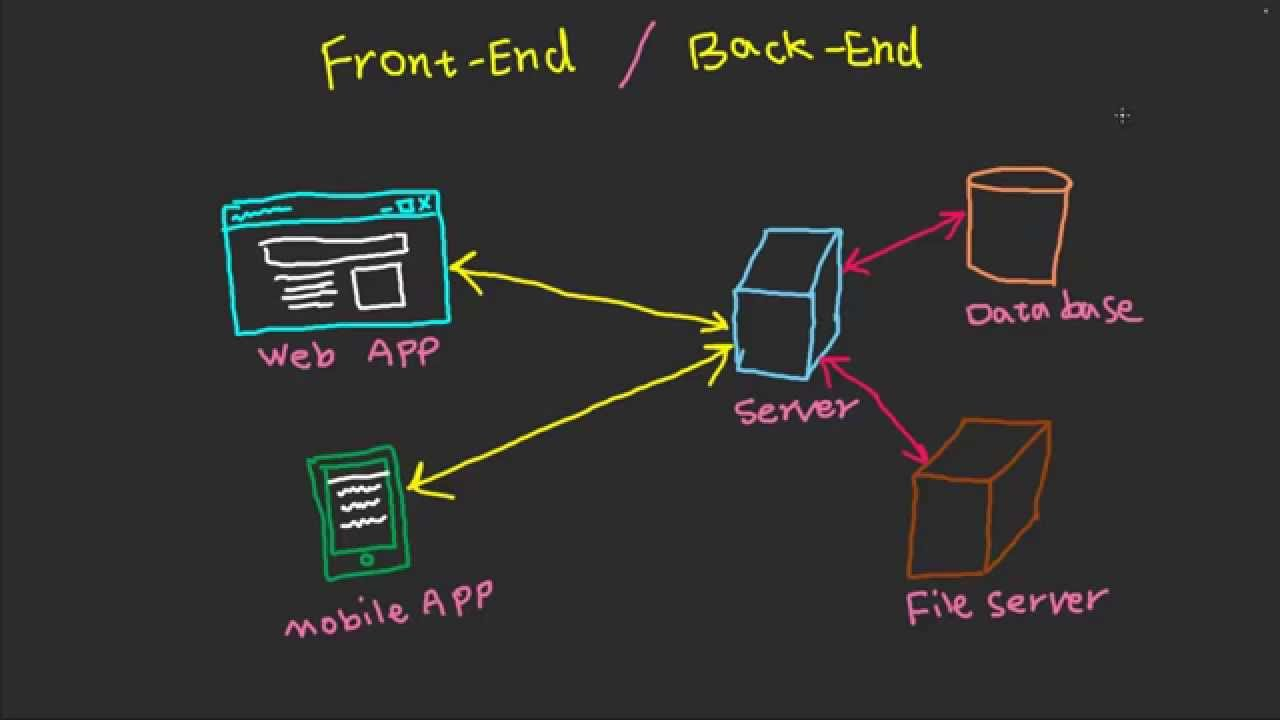
\includegraphics[width=1\textwidth]{figures/1backend.jpg}}
\caption{Backend}
\label{1backend}
\end{figure}

	Pada gambar \ref{1backend} berikut ini dijelaskan mengenai Back-end atau server-side yang merupakan bagaimana sebuah website berkerja, meng-update
dan berubah. back-end adalah sesuatu system yang dimana User tidak akan dapat melihatnya di dalam browser,
seperti Database dan Server. biasanya orang - orang yang bekerja di bagian back-end di panggil atau disebut sebagai
Programmers atau Developer. Back-end developers adalah orang yang paling khawatir tentang hal - hal yang menyangkut keamanan,
struktur sistem dan manajemen konten. sebenarnya para back-end develper juga mengetahui tentang front-end seperti HTML dan CSS.
namun itu bukanlah bidang mereka bekerja. 

\subsection{Backend System}
	Pada system dan metode  yang membuat informasi dapat digunakan secara oromatis untuk mengakses 
pada fungsionalitas system computer backend yang digunakan ke server aplikasi. 
Metode ini juga dapat beroperasi untuk menghubungkan ke system computer backend dan memperoleh 
fungsionalitas untuk menentukan informasi  pada system backend. Dan pada informasi yang diperoleh 
dan dapat dianalisis secara terprogram,dan informasi yang sangat baru dapat dianalisis yang dimana 
informasi dibuat secara terprogram dapat digunakan untuk mengakses fungsionalitas system backend.
Back-end biasanya mengacu pada program dan skrip yang bekerja di dalam server, untuk membuat sebuah 
halaman web yang dinamis dan interatif. Back-end memiliki tugas-tugas yaitu seperti :

\begin{enumerate}
\item Desain Informasi pada web
\item Pemrosesan form
\item Pemrograman dalam database
\item Aplikasi Berbasis Web
\end{enumerate}
Dari tugas - tugas tersebut Back-end memiliki tiga bagian diantaranya yaitu server,aplikasi, dan database
\cite{shapiro2005system}.

\section{Bahasa Pemrograman yang digunakan di Backend}
Pada gambar \ref{2labelgambar} berikut ini dijelaskan bahwa pada Backend terdapat beberapa bahasa programing yang digunakan,
termasuk C, Python, dan lainnya. pada materi di bawah ini terdapat beberapa penjelasan tentang bahasa pemrogramannya.

\begin{figure}[ht]
\centerline{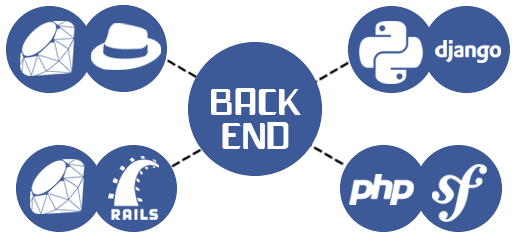
\includegraphics[width=1\textwidth]{figures/1bahasapemrogramanbackend.png}}
\caption{Bahasa Pemrograman yang dipakai di Backend}
\label{2labelgambar}
\end{figure}

\subsection{C}
	Bahasa Pemrograman Backend yang biasa digunakan developer ialah C, C++, dan Java .
Bahasa C adalah suatu perkembangan dari bahasa B yang di kembangkan oleh Ken Thompson pada tahun 1980.
Bahasa C rilis pertama kali ditulis oleh Brian W. Bahasa C, awalnya digunakan oleh sistem operasi UNIX.
Bahasa C adalah bahasa pemrograman tingkat standar, bahasa C memiliki kegunaan yang sering di gunakan
diantaranya untuk membuat perangkat lunak.

\subsection {C++}
	Pengertian C++ adalah `multi-paradigm' artinya anda dapat menulis suatu kode, caranya procedural 
tapi juga bisa menggunakan fungsional,berorientasi objek, dan campuran paradigm suatu pemrograman.  
Bahasa pemrograman C++ ini bisa lebih sulit untuk dipelajari; kita dapat mengembangkan dengan 
menggunakan satu atau lebih dari model ini,  atau kita dapat menggabungkan dengan Bahasa pemrograman lainnya.

\subsection {C\#}
	Sedangkan C\# merupakan sebuah bahasa programming yang simple, modern, OOP dan aman untuk 
penggabungannya dengan beberapa bahasa programming lain
\cite{hejlsberg2003c}.

\subsection {PHP}
 	adalah salah satu server side untuk dirancang khusus untuk aplikasi web dan PHP disisipkan diantara bahasa HTML sebab bahasa server side, maka dieksekusi diserver. sehingga yang kirimkan ke browser adalah hasil jadi dalam bentuk HTML. PHP termasuk Open Source Product dapat diubah disource code dan mendistribusikan secara bebas.

\subsection{Python}
	Python merupakan  bahasa pemrograman yang serba guna atau bersifat open source. 
Python lebih menekankan pada pembacaan  kode agar lebih mudah untuk memahami sintaks. 
Hal tersebut membuat bahasa pemrograman python lebih mudah dipelajari baik pemula maupun untuk yang 
sudah menguasai bahasa pemrograman ini dan dilengkapi dengan fungsionalitas standar besar serta 
komprehensif. Pyhton telah digunakan untuk mengembangkan berbagai macam perangakat lunak, seperti 
internet scipting, system programming, user interfaces, prudect customization,numberic programming. 
Pada saat ini bahasa pemrograman pyhton menduduki posisi 4 atau 5 paling sering digunakan diseluruh dunia.

\subsection{Perl}
	Proxy server ialah suatu komputer atau beberapa komputer yang diletakkan sebagai pelayanan kepada pelanggan yang ingin mengajukan layanan data baik dari pusat komputer(server).
Proxy server sering disebut sebagai media cache terhadap suatu konten website. Di ruang lingkup pendidikan pada laboratorium komputer jaringan di Institusi Sains \& Teknologi ditemukan jaringan yang belum ada penanganan masalah internet yang diakses berkali-kali sehingga bandwidth pada internet tidak efektif, penelitian ini bertujuan  untuk melakukan suatu penyimpanan konten yang diakses ke dalam proxy server kemudian melakukan filter konten menggunakan pemrograman PERL.
Ini dilakukan melalui proxy server, yaitu melalui fungsi pada cachig dan filter pada proxy server dengan menggunakan pemrograman PERL dan regex pada PERL
\cite{pamungkas2017implementasi}.

\subsection{ASP .NET}
	ASP.NET merupakan produk dari teknologi Microsoft untuk pengembangan aplikasi berbasis web dinamis. 
Bahasa pemrograman ini mempermudah pada pemula maupun yang sudah menguasai bahasa pemrograman ini , dikarenakan memberikan solusi pada pengembang untuk mendesign aplikasi web dengan cepat, mudah dan efisien. 
ASP diproses melalui web server dan menghasilkan HTML untuk dikirimkan pada web browser.


\subsection{Java}
	Dalam backend juga menggunaka javascript yaitu suatu format teks untuk mengserialisasi data yang terstruktur yang berasal dari objek literal JavaScripts.Pada JavaScript dapat mewakili dari empat tipe yaitu string, angka, boolean, dan nul, dan ada juga dua tipe terstruktur yaitu objek dan array. Objek kumpulan yang tanpa batas dari nol ata lebih dari nama atau nilai pasangannya, yang dimana nama ialah string sedangkan nilai ialah angka, boolean, objek, dan null. Array yaitu urutan dari nol atau melebihi banyak nilai.

\subsection{Ruby}
	Ruby merupakan bahasa pemrograman yang stabil, dengan menggabungkan bahasa pemrograman favoritnya seperti Perl, smalltalk, Eiffel, dan Lisp.
Membentuk suatu bahasa pemrograman baru yang menyeimbangkan pemrograman fungsional dengan imperatif.
Bahasa pemrograman Ruby mempunyai sistem yang dengan otomatis akan langsung terhapus semua data-data yang tidak terpakai dan tidak digunakan lagi pada memori. 
Platform sistem operasi yang mendukung bahasa pemrograman Ruby yaitu sistem operasi Linux, Unix, Amiga, Symbian, Mac dan Windows.

\section{Database Backend}
	Pada sistem basis data yaitu telah lama dilanda masalah kinerja pada penigkatan dalam penggunaan mainframe atau di dalam aplikasi basis data. Dan solusi untuk masalah ini yaitu dengar membongkar sistem basis data dari komputer mainframe ke komputer backend. Pada komputer itu memiliki penyimpanan disk sendiri, digunakan juga untuk melakukan semuoa operasi data base, dan saling berinteraksi dengan mainframe
\cite{yousefi2008database}.


\section{Arsitektur Three-Tier}
	Didalam masalah arsitektur two-tier telah diupdate ke tingkat tertentu dengan memperluas dari dua tingkat menjadi tiga tingkat.
Arshitektur three-tier akan mengisolisasi pemrosesan data dari lokasi pusat yang dapat dengan mudah diubah tanpa melibatkan dan mepengaruhi klien. Di dalam arsitektur three-tier ini, logika presentasi berada pada tingkat pertama (klien), logika bisnis berada pada 
tingkat menengah, dan yang lainnya seperti database berada di tingkatan ketiga yaitu back-end. Di tingkat menengah dalam
arsitektur three -tier (server aplikasi) akan menangani pemrosesan data dan akan menjadi antarmuka antara front - end (klien) dan
tingkat back-end (database)
\cite{demurjian1986multi}.


\section{Web Service}
	Web Service merupakan penyatuan dari 2 aspek yaitu Web dan Service, yang mana penjelasan Web dan Service akan dijelaskan di bawah ini :

\subsection{Web}
	pertama - tama disini akan dijelaskan tentang Web, Web merupakan website yang berarti 
jaringan yang dapat mengakses situs secara global.

\subsection{Service}
	Service merupakan layanan, yang dimana digunakan untuk melayani dan melakukan pelayanan.
sehingga dari kedua perihal diatas dapat disimpulkan bahwasanya web service adalah sebuah jaringan global yang memiliki pelayanan atau keamanan,
didalam web service user diberikan layanan berupa keamanan dalam berselancar di Internet. 
macam - macam model dari web service adalah sebagai berikut ini :

\begin{enumerate}
\item SOAP (Simple Object Access Protocol)
\item WDSL (Web Service Description Language)
\item RDF (Resource Description Framework)
\item RSS (Really Simple Syndication)
\end {enumerate}
\cite{curbera2001web}.


\section{Backend Developer}
	Orang yang bekerja di bagian back-end atau bisa kita sebut seorang back-end developer adalah seorang programmer yang hanya
memusatkan atau berfokus pada bagian keamanan, desain sistem, dan management data pada sistem. Seorang back-end developer
sangat dibutuhkan dalam melakukan pengembangan sistem atau sebuah aplikasi yang dinamis atau aplikasi yang memiliki data selalu
berubah - ubah, contohnya website yang dinamis seperti facebook dan google.

\section{Backend as a Service}
	Baas adalah sebuah provider untuk web dan mobile app developer untuk dapat mengkoneksikan 
aplikasi mereka ke dalam system penyimpanan cloud backend sekaligus masih tetap melakukan proses yang lain seperti user management, 
mendapatkan notifikasi, bermain social media, dan fitur – fitur lainnya yang terdapat di dalam aplikasi mobile mereka saat ini.

\subsection{Kelebihan yang dimiliki BaaS}
	Tujuan dari BaaS adalah untuk membuat hidup developer menjadi 
lebih mudah. BaaS ada karena kurangnya keahlian dari seorang 
mobile developer dan tingginya tingkat permintaan user untuk 
aplikasi smartphone mereka. berikut ini adalah kelebihannya :

\begin{enumerate}
\item Keuntungan yang efisien
\item Lebih cepat waktu penjualannya
\item Aplikasi didelivery dengan sumber daya yang lebih sedikit
\item Ter-optimisasi untuk mobile dan tablet
\item Aman dan terukur
\item Penggunaan sumber daya API yang umum dipakai
\end{enumerate}

\subsection {Yang dapat anda buat dengan menggunakan BaaS}
\begin{enumerate}
\item Pengembangan Website
\item Mobile Aplikasi, dll
\end{enumerate}
\cite{lane2015overview}.

\section{JSON (JavaScript Object Notation)}
	merupakan sebuah format pertukaran data yang mudah dibaca atau dimengerti dan dituliskan oleh manusia, 
serta JSON memiliki kemudahan untuk diterjemahkan dan juga diubah \(generate\) oleh sebuah mesin \(Computer\).
JSON adalah sebuah format teks yang tidak memiliki ketergantugan pada Bahasa pemrograman manapun karena JSON menggunakan 
gaya penulisannya sendiri yang mana dia menggunakan Bahasa – Bahasa pemrograman yang sudah umum seperti C family, Java, 
JavaScript, Perl, Python dan lainya, dan menjadikannya sebagai sebuah format yang tetap miliknya sendiri.
hal tersebutlah yang menjadikan JSON sebagai format pertukaran data yang ideal didalam dunia pemrograman
\cite{crockford2006application}.


\section{Mobile Backend Starter}
	Backend tidak hanya dipakai oleh web yang dinamis namun akhir - akhir ini google telah menambahkan sebuah layanan yang bernama
`Mobile Backend Starter', google menambahkan layanan tersebut dengan tujuan untuk memudahkan pengguna untuk menggunakan
layanan awan berupa `Cloud Services' dalam sebuah aplikasi mobile yang akan dikembangkan. Ketersediaan dari layanan `Mobile Backend Starter' ini bebas digunakan untuk publik
\cite{soinu2014cloud}.



		




%\chapter[Frontend]
%{Frontend}
%\input{section/1Frontend.tex}


\chapter[Frontend]
{Frontend}
%KELOMPOK 4 Blank-On1
%\begin{enumerate}
%\item Andri Fajar Sunandhar
%\item Cokro Edi Prawiro
%\item Fadila
%\item Sandro Samuel Sinaga
%\end{enumerate}


\section{Definisi Frontend}
frontend bisa disebut tampilan utama dari sebuah website pada frontend biasanya ditampilkan beberapa konten-konten yang bisa diakses oleh pengguna atau user yang menggunakan website tersebut. frontend juga berfungsi untuk user interace dari setiap web site. Biasanya frontend hanya menampilkan fungsi fungsi dari kontent sebuah web site seperti fungsi sebuah tombol untuk mengirim berkas atau untuk menampilkan konten konten yang lainnya dalam website tersebut.

Front-end adalah  segala sesuatu yang menghubungkan antara user dengan sistem back-end. Biasanya merupakan sebuah user interface 
dimana user akan berinteraksi dengan sistem. Pekerjaan yang sering muncul sebagai seorang front-end developer adalah desainer user interface
dan desainer user experience. Seorang front-end developer tidak akan membuat program atau aplikasinya yang berjalan di logic bisnis 
tapi fokusnya akan lebih banyak ke antarmuka, desain grafis (user interface designer) dan bagaimana membuat desain yang nyaman
digunakan oleh user (user experience designer). Bahasa pemrograman yang biasanya digunakan dalam pengembangan front-end adalah HTML.

\subsection{Fungsi Front-end}
Fungsi ini berhubungan langsung dengan pengguna dan berperan penting dalam keseluruhan proses bisnis dalam hal menghubungkan 
back-end dengan pengguna. layanan depan (front-end) bertugas mempresentasikan apa yang sudah dikerjakan oleh back-end
dan menjadi sarana bagi pengguna untuk mendapatkan segala sesuatu yang disediakan dibagian fungsi back-end. Peningkatan fungsi layanan depan yang baik akan mampu meningkatkan kepuasan pengguna\cite{razaq2014sistem}.
\subsection{Programming language on Front-end: Javascript }
Frontend programming language there are various. Such as HTML, CSS, and Javascript. One of them is Javascript. Javascript is language in the form of a script that in its function can run on an HTML document, where throughout history this language is the first scripting language in development / for the web. Javascript is a programming language that provides additional capabilities against the HTML language by allowing the execution of commands on the user side, which is interpreted on the browser side rather than on the server side of the web\cite{alamsyah2003pengantar}.

\subsection{Programming language on Front-end: CSS }
Frontend programming languages other than HTML, Javascript, and others, there is called CSS. CSS stands for Cascading Style Sheet. Cascading Style Sheet itself is a technology used to beautify 
the look of the website pages (sites) that you want. Using the CSS method you can easily change the overall color and appearance of the site you create, as well as to format or change the order of your site quickly\cite{poetra2003tutorial}.

\subsection{Front-end di Android}
Di Android terdapat 2 bagian, yaitu aplikasi front-end dan back-end. Front-end adalah aplikasi yang sudah terinstal dalam perangkat mobile yang digunakan.
Back-end adalah aplikasi pendukung yang berfungsi sebagai penyuplai atau sumber data pada aplikasi front-end. Front-end merupakan suatu penghubung
antara user dengan basisdata yang digunakan untuk melakukan pemrosesan data yang disimpan. Front-end dapat diciptakan menggunakan 
beberapa bahasa program seperti Visual Basic, Visual C++, Visual Foxpro, Java, dan sebagainya. Sedangkan back-end merupakan basisdata itu sendiri.
 Secara garis besar aplikasi Front-end dibagi menjadi 2 kategori, yaitu :
\begin{enumerate}
\item Decision Support Front-end yaitu aplikasi yang hanya menampilkan  dan mencetak informasi yang diambil dari basisdata baik melalui predefined atau user defined Query.
\item  Transaction Processing front-end yaitu aplikasi yang mencakup kemampuan untuk mengedit, menambah, dan menghapus record dari basisdata\cite{nuari2014perancangan}.
\end{enumerate}
\section{Konsep Membangun Aplikasi Frontend Berbasis Web APPML(Application Modeling Language) }
Diperlukan sebuah metode penghubung antara sistem dengan dukungan JSON, XML. Dengan teknik APPML (Application Modeling Language) yang diterapkan pada sebuah aplikasi front-end berbasis HTML 5 tanpa melakukan koneksi database secara langsung, tetapi cukup memanggil service berbasis JSON maka akan diperoleh data atau informasi yang dibutuhkan tanpa harus mengunjungi sistem informasi yang ada secara langsung\cite{triyono2017konsep}.

\section{definisi web serfice }
Webservice terdiri dari 2 kata yaitu Web yang berati websit atau online 
sedangangkan service berarti layanan atau melayani aplikasi berbasis web 
Website adalah suatu sistem perangkat lunak yang dirancang untuk mendukung interaksi antara sisitem pada suatu jaringan.
web service digunakan sebagai suatu fasilitas yang di sediakan oleh suatu website untuk menyediakan layanan berupa informasi kepada 
sistem lain, sehingga sisitem lain dapat berinteraksi dengan sistem tersebut melalui service yang telah disediakan oleh sistem web service.
Webservice menyimpan data informasi dalam bentuk XML, sehingga data tersebut dapat diakses oleh sitemlain miskipun berbentuk platfrom. 
\subsection{keterkaitan web service dan front end }
sebagian besar orang sering berpikir bahwa suatu website dimiliki oleh suatu pihak 
itu merupakan suatu yang disebut dengan website. banyak yang berpikir bahwa aplikasi yamg berbasiskan 
web merupakan suatu aplikasi yang menitik beratkan tampilan front endnya pada suatu web browser 
padahal nyatanya aplikasi berbasis web tidak sepenuhnya menggunakan web browser sebagai tampilan 
frontendnya. menurut Gani pengertian website di sini atalah suatu jaringan yang luas atau keterhubungan 
antara beberapa aplikasi dan atau komponen suatu aplikasi menjadi suatu aplikasi yang baru.

\subsection{Arsitektur Web Service}
\begin{figure}[ht]
\centerline{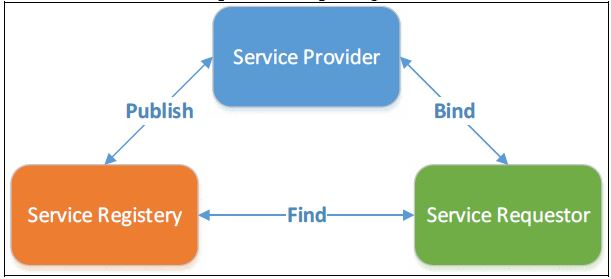
\includegraphics[width=1\textwidth]{figures/1arsitektur.JPG}}

\caption{Arsitektur web service.} 
\label{1arsitektur}
\end{figure}

Gambar \ref{1arsitektur} mendefinisikan arsitektur dari Web Services dimana pada Web Services sendiri terdiri dari Layanan Untuk 
Requestor, Registery dan juga Provider. Dimana kegiatan yang dilakukan untuk setiap layanan pada arsitektur tersebut ialah, `publish' 
untuk Service Registery dan Service Provider. `Bind' untuk Service Provider dan Serviice Requestor , dan juga `Find' untuk Service 
Registery dan Service Requestor. Pada Tabel \ref{1table} dipaparkan bahasa pemerograman yang sering digunakan dalam pembuatan frontend. 
Terdapat tiga komponen utama dari web service, komponen komponen tersebut antara lain :
service Provider, Service Requestor, Service Registry .


\begin{enumerate}
\item service Provider adalah penyedia web service yang berfungsi menyediakan kumpulan webService yang dapat diakses oleh USER atau pengguna.
\item Service Requestor Adalah aplikasi yang bertindak sebagai pengguan yang melakukan permintaan layanan berupa WebService kepada Service Provider.
\item Service Registry Adalah tempat dimana service provider mempublikasikan layanannya. pada arsitektur Webservice, service registry bersipat opsional\cite{kurniawan2015implementasi}.
\end{enumerate}


Pada Tabel \ref{1table} dipaparkan bahasa pemerograman yang sering digunakan dalam pembuatan frontend




\begin{table}[h]
\caption{Bahasa pemerograman yang sering digunakan di Frontend}
\centering
\begin{tabular}{ccccc}
\hline
one&two&three&four&five\\
\hline
Java&Phyton&PHP&Javascript&C++\\
\hline
\end{tabular}
\label{1table}
\end{table}





\chapter[Pengertian Web Service]
{pengertianwebservice}
%Resume tentang Pengertian Web Service

%Kelompok 2 D4 TI / 2B

%Alwan Suryansah				1164033 
%Dinda Ayu Pratiwi				1164034
%Kurnia Sandi					1164042
%Teduh Sanubari					1164054
%Wildan Khaustara Wijaksana		1164058

\documentclass[12pt]{article}
\usepackage{apacite}


\begin{document}

\title{Pengertian Web Service}
\maketitle

Web service ialah terobosan baru dalam sistem terdistribusi dengan Web yang menggunakan teknologi XML, dengan standar protokol  HTTP dan SOAP. Terobosan teknologi Web service muncul untuk mendukung sistem terdistribusi yang memiliki infrastruktur yang berbeda. Infrastruktur yang berbeda ini mampu dihubungkan dengan web service melalui XML sebagai teknologi yang mendukung integrasi berbagai paltform sistem dan aplikasi.
kbhbh
\section{Definisi}

\subsection{Hartati Deviana}
\paragraph{}
Web service adalah suatu komponen perangkat lunak self-containing dan aplikasi modular self-describing yang dapat disiarkan, dialokasikan, dan dijalankan di dalam web. Web service adalah teknologi yang mentransformasikan kemampuan internet dengan cara menambahkan beberapa kemampuan seperti kemampuan transactional web. Apa itu Transactional Web? Transactional Web yaitu kemampuan web dalam hal saling berinteraksi dengan pola program-to-program (P2P). Fokus web selama ini didominasi oleh komunikasi program-to-user dengan interaksi business-to-consumer (B2C), sedangkan transactional web akan didominasi oleh P2P dengan interaksi business-to-business (B2B). \cite{deviana2013penerapan}.

\subsection{Richards Robert}
\paragraph{}
Web service merupakan salah satu implementasi dari teknologi XML (Extensible Markup Language) pada proses pertukaran antara (data exchange) platform yang berbeda sercara berbeda.

\textit{"A Web service is a software system designed to support interoperable machine-to-machine interaction over a network. It has an interface described in a machine-processable format(specifically WSDL).Other systems interact with the Web service in a manner prescribed by its description using SOAP messages, typically conveyed using HTTP with an XML seriali zation in conjunction with other Web-related standards"}.

Menurut Richards, web service dapat digunakan untuk berkomunikasi antara mesin satu dengan mesin yang lain melalui interface perantara yang umumnya berupa WSDL(Web Service Definition Language), layanan ini biasa bekerja pada protokol HTTP dengan bentuk response dan request berupa SOAP messange. SOAP (Simple Object Access Protocol) adalah standar untuk bertukar pesan-pesan berbasis XML melalui jaringan komputer atau sebuah jalan untuk program yang berjalan pada suatu sistem operasi (OS) untuk berkomunikasi dengan program pada OS yang sama maupun berbeda dengan menggunakan HTTP dan XML sebagai mekanisme untuk pertukaran data. Format SOAP message adalah mengikuti frame XML yang terstandarisasi \cite{ihya2011pembuatan}. 

\subsection{Chen, Xi dan Zheng, Zibin dan Yu, Qi dan Lyu, Michael R}
\paragraph{}
Web Service adalah komponen perangkat lunak yang terintegrasi untuk mendukung interaksi antar mesin dengan mesin yang lainya ( komputer ) antar jaringan , layanan web service telah banyak digunakan untuk membangun suatu aplikasi yang berorientasi dengan layanan industri dan akademisi dalam beberapa tahun trakhir , jumlah layanan web yang tersedia untuk umum terus meningkat di internet , Namun  ini menyulitkan pengguna untuk memilih layanan yang tepat di antara banyaknya layanan web services\cite{chen2014web}.

\subsection{Witono, Timotius and Susanto, Raphael}
\paragraph{}
Pengertian sederhana web service adalah aplikasi yang dibuat agar dapat dipanggil atau diakses oleh aplikasi lain melalui internet atau intranet dengan menggunakan XML sebagai format pengiriman pesan. Web service digunakan saat pengguna akan mentransformasi sebuah logik atau sebuah class dan objek yang terpisah dalam satu ruang lingkup yang menjadi satu, sehingga tingkat keamanan dapat ditangani dengan baik\cite{witono201511}.

\subsection{Kurniawan, Erick}
\paragraph{}
Web Service adalah layanan yang tersedia di Internet. Web Service menggunakan format standar XML untuk pengiriman pesannya. Web Services juga tidak terikat kepada bahasa pemrograman atau sistem operasi tertentu (Ethan Cerami, 2002). Web Services adalah antar muka yang mendeskripsikan koleksi yang dapat diakses dalam jaringan menggunakan format standar XML untuk pertukaran pesan. Web Services mengerjakan tugas yang spesifik. Web Services dideskripsikan menggunakan format standar notasi XML yang disebut services description (Gottschalk, 2002)\cite{chen2014web}.

\subsection{Sarbini, Riska Nurtantyo}
\paragraph{}
Web service merupakan satuan diskrit dari fungsionalitas programatis yang diekspos 
kepada client via protokol komunikasi, dan format data standar bernama HTTP dan 
XML. Protokol ini mengatasi masalah komunikasi lintas internet dan lintas 
firewall tanpa beralih ke solusi superior yang memerlukan port-port komunikasi 
tambahan yang harus dibuka untuk akses eksternal. Dikarenakan web service mamiliki fungsi untuk menformat dan menguraikan pesan XML\cite{sarbini2015pengembangan}. 

\subsection{M. Shalahuddin dan Rosa A.S.}
\paragraph{}
Web Service merupakan suatu sistem yang menyediakan pelayanan yang dibutuhkan oleh klien. Klien dari web service tidak hanya berupa aplikasi web, tetapi juga bisa sebuah aplikasi enterprise. Jadi web service tidak sama dengan web server, bahkan sebuah aplikasi web pada web server dapat menjadi klien dari web service\cite{inayah2014aplikasi}.

\subsection{Gottschalk (2002)}
\paragraph{}
Web Service adalah teknologi yang mengubah kemampuan internet dengan menambahkan kemampuan transactional web, yaitu kemampuan web untuk saling komunikasi dengan pola program to program (P2P). Fokus web selama ini didominasi oleh komunikasi program to user dengan interaksi business to costumer (B2C), sedangkan stransactional web akan didominasi oleh P2P dengan interaksi business to business\cite{fauziah2014aplikasi}.


\subsection{Slameto, Andika Agus}
\paragraph{}
Web service adalah suatu sistem perangkat lunak yang dirancang untuk mendukung interoperabilitas dan interaksi antar sistem pada suatu jaringan. Web service digunakan sebagai suatu fasilitas yang disediakan oleh suatu web site untuk menyediakan layanan (dalam bentuk informasi) kepada sistem lain, sehingga sistem lain dapat berinteraksi dengan sistem tersebut melalui layanan-layanan (service)yang disediakan oleh suatu sistem yang menyediakan web service. Web service menyimpan data informasi dalam format XML, sehingga data ini dapat diakses oleh sistem lain walaupun berbeda platform, sistem operasi, maupun bahasa compiler\cite{slameto2015penerapan}.

\subsection{Jurnal Masyarakat Informatika}
\paragraph{}
web service adalah antarmuka yang mendeskripsikan sekumpulan operasi yang dapat diakses dalam sebuah jaringan melalui pesan XML yang telah distandartkan.xml iyalah bahasa markup yang sudah terintregrasi dengan web service. W3C mendefinisikan web service sebagai sebuah sistem perangkat lunak yang dirancang untuk mendukung inter operasi mesin ke mesin di sebuah jaringan.  Web service merupakan komponen perangkat lunak loosely coupled, dapat diguna ulang, membungkus fungsionalitas diskret, didistribusikan, dan diakses secara programatik melalui protokol internet standart . dan sangat di di perhatikan di bidang informatika \cite{saputra2integrasi}.

\subsection{Jurnal Sistem dan Teknologi Informasi}
\paragraph{}
Web service menurut World Wide Web Consortium (W3C) (2004), organisasi yang mengembangkan standar-standar dalam dunia web, mendefinisikan web service sebagai "\textit{“a software system designed to support interoperable machine-to-machine interaction over a network. It has an interface described in a machine-processable format (specifically WSDL). Other systems interact with the Web service in a manner prescribed by its description using SOAP messages, typically conveyed using HTTP with an XML serialization in conjunction with other Web-related standards.” }"(Lucky,2008).

Berdasarkan definisi dari W3C dapat disimpulkan bahwa web service merupakan aplikasi yang dibuat agar dapat dipanggil atau diakses oleh aplikasi lain melalui internet maupun intranet dengan menggunakan XML sebagai format pengiriman pesan\cite{prasetya2013perancangan}.

\subsection{Pengertian Web Service menurut Hartono, Fajar Fani and Hendry, H and Somya, Ramos}
\paragraph{}
Web Service dapat diartikan sebuah antar muka atau dalam bahas inggris yaitu interface  yang berarti menggambarkan sebuah sekumpulan operasi-operasi yang kemudian dapat diakses melalui jaringan, misalnya internet dalam bentuk pesan “Extensible Markup Language (XML)”. Web Service juga menyediakan standar komunikasi dalam berbagai software yang berbeda-beda, dan dapat berjalan di berbagai platform maupun framework\cite{hartono2013aplikasi}.

\subsection{Pengertian Web Service Menurut Kasaedja, Bramwell A and Sengkey, Rizal and Lantang, Oktavian A}
\paragraph{}
O’Reilly menerbitkan sebuah buku, David A Chappel dan Tyler Jewell sebagai penulis mengartikan bahwa web service adalah suatu kumpulan logika bisnis dalam internet yang dapat di akses melalui protocol internet. Dalam buku tersebut juga dijelaskan bahwa terdapat tiga komponen teknologi dalam Web service yaitu, Simple Object Acces Protocol (SOAP), Web Service Description Language (WSDL), dan Universal Description, Discoveri, Integration (UDDI)\cite{kasaedja2014rancang}.

\subsection{Hamdani, Hamdani and Haviluddin, Haviluddin and Darmawangsa, Ngurah Satria}
\paragraph{}
Web service diartikan sebagai sebuah antar muka (interface) yang menggambarkan sekumpulan operasi-operasi yang dapat diakses melalui jaringan, misalnya internet, dalam bentuk pesan XML. Web service diartikan sebagai sepotong atau sebagian informasi atau proses yang dapat diakses oleh siapa saja, kapan saja dengan menggunakan piranti apa saja, tidak terikat dengan sistem operasi atau bahasa pemrograman yang digunakan.

\subsection{Novi Nuari}
\paragraph{}
Webservice ialah suatu sistem perangkat lunak yang dibangun guna mendukung interaksi antar mesin dalam suatu jaringan. Webservice digunakan sebagai suatu fasilitas yang disediakan oleh suatu website untuk menyediakan layanan (dalam bentuk informasi) kepada mesin lain, sehingga mesin lain dapat berinteraksi dengan mesin tersebut melalui layanan-layanan (service) yang disediakan oleh provider\cite{nuari2014perancangan}.

\subsection{Wellem, Theophilus}
\paragraph{}
Web service merupakan suatu software sistem yang mendukung interaksi yang interoperable dari machine to machine melalui jaringan (World World Wide Consortium).  (Stencil Group). Dengan suksesnya Web service sebagai suatu standar teknologi software, memberikan peluang yang besar untuk pengembangan aplikasi terdistribusi melalui Internet.
Web service sebagai suatu standar teknologi software, memberikan peluang yang besar untuk pengembangan aplikasi terdistribusi melalui Internet. Saat ini Web service tidak hanya dapat diakses melalui komputer saja, tetapi juga dapat diakses melalui mobile device, seperti telepon seluler dan PDA, sehingga memungkinkan diciptakannya layanan mobile menggunakan Web service dan aplikasi mobile yang menggunakan Web service ini\cite{wellem2015perancangan}.

\subsection{Jurnal Informatika Kenali, Eko Win }
\paragraph{}
Menurut Gerami (2002) web services adalah suatu layanan-layanan yang disediakan oleh internet, dengan menggunakan pengiriman pesan format Extensible Markup Language (XML), dan tidak saling bergantung pada satu sistem operasi atau Bahasa pemrograman. Komponen dalam web service memiliki 3 arsitektur, dan masing-masing komponen tersebut adalah Service provider, Service requestor, dan Service registry\cite{kenali2015desain}. 

\subsection{Sigit, Haris Triono and Sulistiyono, Sulistiyono}
\paragraph{}
Web Service adalah bagian dari perangkat lunak yang membuat dirinya tersedia melalui internet dan menggunakan sistem pesan XML standar. XML digunakan untuk mengkodekan semua komunikasi ke Web Service. Misalnya, klien memanggil Web Service dengan mengirim pesan XML, kemudian menunggu tanggapan XML yang sesuai. Karena semua komunikasi ada dalam XML, Web Service tidak terkait dengan sistem operasi atau bahasa pemrograman manapun. Web Service adalah kumpulan protokol dan standar terbuka yang digunakan untuk pertukaran data antara aplikasi atau sistem\cite{sigit2017desain}.  

\section{Manfaat}

Layanan web memungkinkan penyedia layanan dan vendor untuk menjual layanan mereka dengan memublikasikannya
Yang di akses melalui World Wide Web.
Manfaat dari layanan web kita dapat berbagi data walaupun memiliki jarak yang jauh dan dapat mempermudah membagi suatu data dalam sebuah pekerjaan
interoperabilitas. Manfaat ini berasal dari antarmuka XML standar dan deskripsi akses
diberikan oleh WSDL (Web Services Description Language). Deskripsi WSDL sangat membantu dalam perusahaan
integrasi aplikasi, integrasi B2B (menyelesaikan tantangan antara bisnis dan bisnis partner, seperti customer, supplier, bank, dan jasa transportasi ) \cite{ferris2003web}.

\section{Arsitektur Web service}

\subsection{\textit{Service Oriented Architecure (SOA)} }

\paragraph{}
Konsep arsitektur yang mendasari teknologi Web service adalah Service Oriented Architecure (SOA), SOA mendefinisikan 3 peran berbeda yang menunjukkan peran dari masing-masing komponen dalam system, yaitu (W3C, 2004) :
\begin{itemize}
\item \textit{Service provider}, yaitu suatu entitas yang menyediakan interface terhadap sistem yang menjalankan suatu sekumpulan tugas tertentu.
\item \textit{Service requestor}, yaitu suatu entitas yang meminta/memperoleh (dan menemukan) \textit{software service} dalam rangka meyelesai kan suatu tugas tertentu atau menyediakan solusi bisnis tertentu.
\item \textit{Service registry}, yaitu entitas yang bertindak sebagai penyimpan (\textit{repository}) suatu \textit{software service} yang dipublikasikan oleh \textit{service provider}\cite{hidayat2014penerapan}.
\end{itemize}

\subsection{Jurnal Masyarakat Informatika}

\paragraph{}
Web service dibangun dari tiga komponen unsur utama, yaitu service provider, service registry, dan service requestor. Komponen-komponen tersebut saling berinteraksi melalui komponen web service itu sendiri, yang berupa deskripsi dan implementasi layanan dan prasarana. Dan juga terdapat tiga macam operasi yang memungkinkan komponen komponen tersebut untuk dapat saling berinteraksi, yaitu publish, find, dan bind. Keterkaitan antara peran, operasi, dan komponen web service \cite{saputra2integrasi}.

\subsection{Arsitektur RESTful Web services}
\paragraph{}
Berikut merupakan langkah-langkah yang dilakukan dalam model dasar RESTful Web services (HostBridge, 2009):
\begin{enumerate}
\item Query Request Provider melalui HTTP dengan menggunakan URI (Uniform Resource Identifier). Request menggunakan methods (metode) HTTP untuk menentukan apakah request tersebut dimaksudkan untuk Create (menciptakan), Read (membaca), Update (memperbarui), atau Delete (menghapus) data.
\item HostBridge mengembalikan sebuah dokumen dalam bentuk XML untuk Requester (pemohon) dengan CICS data enclosed\cite{arsana2014rancang}.
\end{enumerate}



\section{Kesimpulan}

\paragraph{}
Dari berbagai definisi tersebut dapat disimpulkan bahwa web service merupakan middleware sebuah internet yang memungkinkan berbagai sistem untuk saling berkomunikasi tanpa terpengaruh pada platform. Web service membungkus operasi-operasi ke dalam sebuah antarmuka yang ditulis dalam notasi XML. Antarmuka ini menyembunyikan detil implementasi dari layanan. Pertukaran informasi yang terjadi dalam web service juga menggunakan pesan dalam format XML \cite{saputra2integrasi}.


\bibliographystyle{apacite}
\bibliography{references}

\end{document}


\chapter[Port]
{Port}
%PORT

%NAMA KELOMPOK 5
%Ajis Trigunawan		1164031
%Alimu Dzul Ikroom		1164032
%Muhammad Hanafi		1164092
%Riki Karnovi			1164052
%Yoga Sakti Hadi P		1164059

\section{PORT}
\subsection{Pengertian Port}
\paragraph{}
\hspace{1cm}
Port adalah tatacara yang memberi ijin sebuah komputer yang memberi dukungan untuk beberapa bagian koneksi dengan komputer yang lain. Port juga dapat mengenali sebuah aplikasi dan layanan yang sedang menggunakan koneksi di dalam sebuah jaringan TCP/IP. Sehingga port juga mengenali salah satu prosses yang di mana server memberikan layanan terhadap klien yang meminta layanan tersebut. Port adalah salah satu media penghubung untuk melewatkan atau mengirim data masuk atau keluar baik pada sebuah komputer maupun dalam penggunaan jaringan komunikasi. Port pada salah satu penggunaannya pada jaringan komunikasi merupakan nama yang diberikan pada titik akhir koneksi. Nama port yaitu berupa angka angka sebagai pembeda tiap  jenis port. Contoh dari penamaan port yang dipakai pada web sebagai transportasi data yaitu port 80.


\subsection{Jenis-jenis Port}
Pada terminologi komputer ada dua jenis port yaitu:
\subsubsection {Port Fisik}
\paragraph{}
\hspace{1cm}
Port Fisik, adalah colokan/slot dibagian belakang cpu sebagai output-input dari komputer ke hardware pendukung lainnya. \\
\begin{enumerate}
\item Port SCSI (small computer system interface) adalah port berfungsi untuk melakukan transmisi data secara cepat dan dapat dipakai untuk 7 alat sekaligus atau “daisy chain“. Contoh daisy chain : dari SCSI kontroller kemudian disambungkan ke perangkat hardisk drive eksternal, dari HDD eksternal disambungkan secara seri ke perangkat yang lain.
\item Port Paralel adalah  salah satu jenis port pada komputer yang digunakan untuk berkomunikasi dengan peralatan luar untuk mengirim data digital dimana setiap bit menggunakan jalur yang terpisah. Pada Port paralel digunakan untuk mentransmisikan data dengan jarak yang pendek dengan cepat karena pemindahan informasi dapat dilakukan secara bersamaan. Contoh penggunaan port paralel yaitu untuk menghubungkan disk eksternal dan printer.
\item Port midi Instrument Digital Interface biasanya disebut midi ialah sebuah sistem piano yang menggunakan synthesizer, dapat mengeluarkan suara instrument music yang lumayan bagus dari elemen music itu sendiri.
\item Port serial port ini biasanya sedikit rumit dalam system kinerjanya , port ini sedikit sangat lambat dalam mengirim data biasanya mengirim data secara satu persatu 
\end{enumerate}
\subsubsection {Port Logika}

\paragraph{}
\hspace{1cm} 
Port Logika atau non fisik, adalah port pada jaringan yang digunakan sebagai jalur penghubung ke komputer lain. TCP atau biasa disebut Transmission Control Protocol adalah bagian dari salah satu jenis protokol yang didalam protokol ini memungkingan terjadinya komunikasi anatara komputer satu dengan yang lainnya, dan dapat pula saling bertukar data. TCP ini berada pada lapisan transport pada 7 lapisan yang ada yang berasal dari OSI, dan pada protokol TCP ini beriorientasi pada sambungan (connection-oriented) sehingga dapat di andalkan (reliale).

\paragraph{}
\hspace{1cm}
Konsep TCP/IP adalah kebutuhan dari DoD (Departement of Defense) AS untuk berlangsungnya komunikasi di antara berbagai komputer yg telah ada. Komputer DoD ini seringkali harus berhubungan antara satu organisasi peneliti dengan organisasi peneliti lainnya, dan harus tetap berhubungan sehingga pertahanan negara tetap berjalan tanpa kendala selama terjadi bencana, seperti ledakan nuklir, gangguan radio. Pada tahun 1969 dilakukan penelitian tentang protokol TCP/IP. Tujuan dari penelitian ini adalah sebagai berikut :\\
1.	Diciptakannya protokol-protokol umum, DoD memerlukan suatu protokol yg dapat dipakai untuk semua jaringan. \\
2.	Meningkatkan efisiensi komunikasi. \\
3.	Dapat dipadukan dengan teknologi WAN (Wide Area Network) yg telah ada. \\
4.	Mudah dipakai dan dikonfigurasi. \\


\paragraph{}
\hspace{1cm}
Karakteristik dari TCP adalah :
Reliable memiliki arti yaitu data yang ditransfer ke tempat tujuan,  dengan urutan yang sama seperti saat dikirimkan.
Berorientasi sambungan (connection-oriented) ialah dimana sebelum data bisa ditransmisikan antara dua host, dua proses yang sedang berjalan pada lapisan aplikasi ini harus melakukan kesepakatan untuk membuat tahap koneksi terlebih dahulu. Koneksi TCP bisa ditutup dengan menggunakan proses terminasi koneksi TCP (TCP connection termination). Aplikasi-aplikasi yang menggunakan TCP yaitu:

\begin{enumerate}
\item WWW adalah kumpulan layanan dan dokumen yang menjadi lapisan terluar dari Internet yang berfungsi sebagai penyedia data dan informasi berupa gambar, suara, video dan animasi. 
\item Archie adalah sebuah sistem pencarian  yang berfungsi untuk mengumpulkan file indeks di internet. Archie hanya berguna untuk mencari file. 
\item Wide Area Information Server (WAIS) adalah sebuah sistem pencarian didalam internet yang berbasis sistem operasi UNIX yang bisa digunakan untuk mencari informasi berbentuk dokumen.\\
\end{enumerate}
\paragraph{}
\hspace{1cm}
User Datagram Protocol (UDP) adalah sebuah protokol transport yang menggunakan port dan menyediakan konektivitas end-to-end antara aplikasi server dan aplikasi client . UDP berbeda dengan TCP, yaitu UDP tidak menjamin pengiriman datanya, oleh karena itu aplikasi harus mengimplementasikan mekanisme error recovery-nya sendiri.\\
\paragraph{}
\hspace{1cm}
Kegunaan UDP : \\
UDP merupakan singkatan dari user datagram protocol, suatu protkol dilapisan transport yang menyediakan  layanan pengantar connectionless dengan usaha yang terbaiknya, UDP biasaya bekerja dengan model client atau server, diterapkan juga di Komputer dan pada ponsel berbasis system operasi, Aplikasi UDP dapat menghasilkan IP Address pada ponsel sehingga ponsel dapat terkoneksi dengan komputer menggunakan protokol IP.UDP tingkatannya di atas Ip karena sifatnya connectionless.\\

Kelemahan UDP :
\begin{enumerate}
\item UDP tidak akan menyediakan mekanisme penyanggaan dari data yang masuk ataupun data yang keluar. Tugas buffering merupakan tugas yang harus dikerjakan oleh protokol lapisan aplikasi yang sedang berjalan di atas UDP.
\item UDP tidak akan menyediakan mekanisme segmentasi data yang besar ke dalam segmen - segmen data, seperti yang terjadi dalam protokol TCP. Karena itulah, protokol lapisan aplikasi yang sedang berjalan di atas UDP wajib mengirimkan data yang berukuran lebih kecil atau tidak lebih besar dari nilai Maximum Transfer Unit (MTU) yang dimiliki oleh sebuah interface di mana data tersebut dikirim. Karena, jika ukuran paket data yang dikirim lebih besar dibandingkan nilai MTU, paket data yang dikirimkan bisa saja terpecah menjadi beberapa fragmen yang akhirnya tidak jadi terkirim dengan benar.
\item UDP tidak akan menyediakan mekanisme flow-control, seperti yang dimiliki oleh TCP.
\end{enumerate}

\paragraph{}
\hspace{1cm}
Port TCP dan UDP dalam pengklasifikasian penomorannya di bedakan menjadi tiga jenis
\begin{enumerate}
\item Well-known Port Merupakan port yang dipakai secara internal oleh sebuah system windows, seperti contoh port yang digunakan untuk pengkoneksian internet, service,FT dan lain sebagainya. Port yang digunakan pada penomoran ini adalah port 0 sampai dengan port 1023. Penomoran port yang berada dalam lingkup well-known port, selalu menggambarkan jaringan yang sama, dan ditetapkan oleh Internet Assigned Number Authority (IANA).
\item Registered Port yaitu port-port yang dipakai oleh vendor-vendor jaringan atau komputer yang berbeda, dimana bertujuan  untuk mendukung sistem operasi dan aplikasi yang dibuatnya. Range dari registered port berkisar dari 1024 sampai 49151. Registered port terdaftar pada organisasi dunia dibidang jaringan komputer yaitu IANA (Internet Assigned Number Authority).Salah satu contoh penggunaan registered port yaitu untuk layanan aplikasi seperti port 1194 untuk Open VPN  dan port 1080 untuk SOCKS proxy.
\item Dynamically Assigned Port adalah sebagian dari port yang telah ditetapkan oleh sistem operasi atau aplikasi yang akan digunakan pengguna untuk meminta suatu permintaan atau layanan sesuai dengan yang di perlukan olehnya. Dynamically Assigned Port juga dapat di perkirakan sekisar 1024 sampai 65536 dan dapat digunakan atau dilepaskan oleh pengguna sesuai kebutuhannya.
\end{enumerate} 

\paragraph{}
\hspace{1cm}
Sesuai dengan kegunaan sebuah Port yaitu media penghubung untuk melewatkan data masuk atau keluar pada jaringan komunikasi. Sebagai contoh jenis-jenis port yang digunakan pada beberapa protokol jaringan :\\
\begin{enumerate}
\item HTTP (Hypertext Transfer Protocol) menggunakan port 80.
\item HTTPS (HTTP Secure) menggunakan port 443.
\item FTP (File Transfer Protocol menggunakan port 21.
\item SSH (Secure Shell) menggunakan nama port 22.
\item Telnet menggunakan port 23.
\item IMAP (Internet Message Access Protocol) menggunakan port 143.
\end{enumerate}

\paragraph{}

Tabel 1 Perbedaan UDP dan TCP\\
\begin{tabular}{|p{4.5cm}|p{5cm}|p{5cm}|}

\hline
Karakteristik/Deskripsi & UDP & TCP \\
\hline
Deskripsi Umum & "Pembungkus paket" yang
memiliki kecepatan tinggi
namun rendah dalam
fungsi. &Protokol dengan fitur
lengkap yang
memungkinkan aplikasi
untuk mengirim data
dengan terpercaya tanpa
khawatir tentang masalah
pada network layer.\\
\hline

\hline
Data Interface Ke
Aplikasi & Message base-based dikirim
dalam paket dengan ciri
tersendiri oleh aplikasi. & Stream-based; Data dikirim
oleh aplikasi tanpa
struktur khusus.\\
\hline

\hline
Pengiriman Ulang & Tidak dilakukan. Aplikasi
harus mendeteksi
kehilangan data dan
mengirim kembali jika
dibutuhkan. & Pengiriman dari seluruh
data telah diatur, dan
kehilangan data akan
dikirim kembali secara
otomatis.\\
\hline

\hline
Fitur yang
disediakan untuk
mengatur flow o f
Data & Tidak ada. & Flow control menggunakan
sliding windows,
pengaturan ukuran jendela
heuristics, algoritma
penghindar kemampatan.\\
\hline

\hline
Overhead & Sangat kecil. & Kecil, tetapi lebih besar dari
UDP.\\
\hline

\hline
Kecepatan
pengiriman & Sangat tinggi. & Tinggi tetapi tidak setinggi
UDP.\\
\hline

\hline
Kesesuaian
kuantitas data & Kuantitas data kecil hingga
sedang. & Kuantitas data kecil hingga
sangat besar.\\
\hline

\end{tabular}



\subsection{Fungsi Port}
\paragraph{}
\hspace{1cm}
Port mempunyai fungsi sangat vital dalam sebuah jaringan sebagai pintu masuk atau jalur yang digunakan untuk melakukan koneksi masuk dan keluar ke komputer lain pada jalur komunikasi. Setiap port mempunyai fungsi masing masing contohnya sebagai berikut:
\begin{enumerate}
\item Port 21 adalah port FTP yang berfungsi untuk tukar menukar data dalam suatu jaringa.
\item Port 22 adalah port SSH yang berfungsi untuk  melakukan koneksi amandalam suatu jaringan.
\item Port 80 adalah port Http yang berfungsi untuk mentransfer dokumen dalam World Wide Web (WWW).
\item Port 81 adalah port yang digunakan sebagai Port altenatifhosting website ketika Port 80 diblok.
\item Port 23 adalah port yang digunakan untuk Telnet . Port 23 digunakan oleh client telnet untuk berhubungan dengan server telnet.
\item Port 25 adalah port yang digunakan ketika pengirim email  mengirim email ke server email.
\item Port 110 adalah POP Server  jika menggunakan Mail server dan pengguna login ke dalam mesin tersebut menggunakan POP3 (Post Office Protokol) atau IMAP4 (Internet Message Access Protocol) untuk menerima emailnya, sedangkan POP3 merupakan protokol untuk mengakses mail box.
\item Port 3389 adalah Remote Desktop Port yang  mempunyai fungsi untuk remote desktop di dalam sistem operasinya Windows XP.
\item Port 389 adalah LDAP Server LDAP atau Protokol Akses Direktori Ringan yang telah
menjadi populer untuk akses Direktori, Nama, Telepon, dan Alamat direktori.
\item Port 143, IMAP4 digunakan untuk Mail Server dimana disitu terdapat tiga komponen antara lain MTA (Mail Transfer Agent), MDA (Mail Dilivery Agent), dan MUA (Mail User Agen). Zimbra adalah software opensource mail server yang sering digunakan karena mudahnya dalam instalasi dan pengelolaannya, sehingga di masa depan kemungkinan akan semakin umum dan popular penggunannya postfix, sendmail, dan qmail adalah beberapa contohnya.
\item Port 443, atau biasa disebut port HTTPS webserver (SSL) yang digunakan untuk menerima permintaan dari HTTP.
\item Port 5631 dapat menjalankan server PCAanywhere menggunakan internet untuk menghubungkan PC dari jarak yang tidak dekat.
Sedangkan 
\item Port 5900 dapat menjalankan sebuah server yaitu VNC yang berguna untuk menjalankan sebuah server dari jarak jauh.
\item Port 111 atau disebut juga port portmapper digunakan oleh Network Information Service atau NFS.
\item Port 3306 merupakan port yang biasanya para programmer gunakan untuk mengelola database karena port ini terhubung dengan Mysql
\item Port 1080 adalah Socks Proxy Server.
\item Port 3128 adalah Server Proxy Squid.
\item Port 3306 adalah Server MySQL.
\item Port 5432 adalah Server PostgreSQL.
\item Port 6000 mencakup port 6000 - 6009 dan X11 TCP port untuk meremotenya. Dapat mensupport berbagai macam tampilan yang memiliki port single.
\item Port 6346 Gnutella, gnutella ialah protocol yang dapat membagi kertas dan mempunyai penyimpanan sendiri, tersedia diunduh bagi semuanya
\item Port 6667 sejenis IRC yang merupakan perangkat lunak server, yang memungkinkan bertukar pesan teks secara real time.
\item Port 6699 memungkinkan orang banyak saling berbagi informasi melalui dunia maya dan  merupakan sistem file sharing peer-to-peer.
ini merupakan contoh tabel \ref{table:contoh} ukuran kecil.


\end{enumerate}


\chapter[Aplikasi Web Service]
{Aplikasi Web Service}
%Nama Kelompok 1
%\begin{enumerate}
%\item Farid Ariyanto Saputra
%\item Nurgivani Syarifatul Husna
%\item Velariza Alvioletta
%\item Yogi Aditya Saputra
%\end{enumerate}


\section{REST}
\subsection{Pengertian REST}
REST atau singkatan dari Representational State Transfer adalah salah satu model arsitektur web yang memiliki aturan berupa interface yang seragam sehingga jika diterapkan dalam web service akan meningkatkan dan memaksimalkan kinerja dalam web sevice, terutama dalam performa dan kemudahan dalam memodifikasi. Dalam arsitektur REST, data-data serta fungsinya dianggap sebagai sumber daya yang biasa di akses melalui URI, yang merupakan singkatan dari Uniform Resource Identifier yang biasanya berupa link pada web.
\subsection{Konsep Kerja REST}
REST merupakan salah satu jenis web service yang menerapkan konsep perpindahan antar state. Jika digambarkan state bisa dikatakan seperti, saat browser meminta suatu halaman web, lalu server akan mengirimkan state halaman web yang diminta kepada browser. (Tidwell, D., 2001) Begitu juga REST mempunyai konsep kerja, dengan bernavigasi dengan link-link HTTP untuk melakukan suatu aktivitas tertentu, seakan telah terjadi perpindahan state, dari state satu ke state lainnya. Perintah  HTTP yang biasanya digunakan adalah fungsi GET, POST, PUT dan DELETE. Respon yang akan dikirim berupa hasil dalam bentuk XML yang sederhana tanpa ada protokol pembagian paket data supaya informasi yang diterima lebih mudah dibaca dan tidak ada pemecahan data pada pengguna atau client.
\subsection{Arsitektur REST}
Representational State Transfer (REST)
\begin{itemize}
\item Aritektur REST \\
REST adalah penyederhanaan dari HTTP. HTTP sering menjadi sesuatu yang tidak diperlukan atau sesuatu yang menyulitkan. Tetapi, dalam beberapa tahun sekarang, dengan kembalinya prinsip REST telah mengindikasikan bahwa HTTP telah cukup baik di atas segalanya.
\item API Flexibility dan Simplicity 
\item Keuntungan Arsitektur REST 
\item Representasi JSON (JavaScript Object Notation) 
\end{itemize}
\subsection{Perintah Dalam REST}
Perintah HTTP dalam REST antara lain :
\subsubsection{GET}
Dalam layanan RESTful webservices terdapat pemetaan metode HTTP yang salah staunya terdiri dari GET. GET merupakan salah satu fungsi CRUD dalam RESTful webservices. Fungsi GET adalah untuk menyediakan layanan read-only pada resource. Untuk kode respons sukses dan error yang digunakan untuk perintah GET adalah 200 untuk kode sukses dan 404 untuk kode error. 

POST, salah satu perintah HTTP yang berfungsi untuk membuat resource baru.
PUT, salah satu perintah HTTP yang berfungsi untuk memperbaharui resource yang sebelumnya sudah dibuat.
DELETE, salah satu perintah HTTP yang berfungsi menghapus resource yang telah di buat.
\subsubsection{PUT}
PUT merupakan metode http request yang biasanya untuk melakukan update data sumber daya. Put digunakan untuk mengganti sumber daya asli pada interface dengan prinsip rest dengan definisi metode http. Permintaan yang dihasilkan berfungsi untuk memperbarui dengan cara  mengidentifikasi permintaan uri atau dalam artian transfer representasi baru dari sumber daya dari klien ke server akan meminta alih-alih mentransfer atribut sumber daya sebagai seperangkat nama parameter dan nilai pada permintaan uri.
\subsubsection{DELETE}
Dalam layanan web RESTful, ada pemetaan antara metode HTTP  yang salah satunya ada perintah DELETE. DELETE. DELETE biasa digunakan untuk removes a resource atau menghapus sumber daya. Untuk kode respons sukses dan error yang digunakan untuk perintah DELETE adalah 200 untuk kode sukses dan 400 atau 404 untuk kode error atau gagal. 
\subsubsection{POST}
HTTP POST adalah salah satu layanan request dalam RESTful. Penggunaan HTTP POST merupakan suatu layanan yang digunakan ketika ingin membuat resource baru atau sumber daya baru. Pada sisi client, request di proses dapat dengan menambahkan resource yang teridentifikasi melalui body sebagai sub body dengan resource dalam request URL(Uniform Resource Language).

\section{HTTP Status Code}
\subsection{200 (OK)}
HTTP Status Code 200 memiliki arti permintaan yang dilakukan oleh pengguna telah sukses dieksekusi. Didalam RESTful, HTTP Status Code 200 sering digunakan untuk indikasi sukses dalam melakukan permintaan dari sisi client. Berbeda dengan 204, Status 200 mengembalikan informasi tergantung metode yang digunakan.
Sedangkan pada Status 204, selalu mengirimkan informasi dengan metode PUT, POST, maupun DELETE.
\subsection{201 (Accepted)}
Kode 202 (Accepted) artinya request diterima tapi server tidak melakukan apapun. Kode 202 juga biasa digunakan untuk tindakan yang prosesnya lama. Maksudnya , permintaan telah diterima untuk di proses, tetapi proses belum selesai. 
Maksud dari itu semua juga, server menerima permintaan dari beberapa proses lainnya (misalkan batch-oriented proses yang hanya berjalan sehari sekali) tanpa membutuhkan agen user penghubung server hingga proses selesai.
\subsection{202 (Created)}
Sebuah rest api akan merespon dengan kode status 201 setiap sebuah koleksi diciptakan, atau menambahkan toko, sumber daya baru atas permintaan klien. Mungkin juga ada waktu ketika sumber daya baru dibuat sebagai hasil dari beberapa tindakan pengontrol, yang dalam hal ini 201 juga akan menjadi respons yang tepat dan akurat.
\subsection{204 (No Content)}
Kode status 204 (No Content) biasanya dikirim sebagai respons atas permintaan PUT, POST, atau DELETE, ketika API REST menolak untuk mengirim sebuah pesan status kembali atau perwakilan apa pun di response message’s body.\\
Respons 204 TIDAK HARUS menyertakan message’s body, karena selalu diakhiri oleh baris yang kosong pertama setelah bidang header.

\chapter[Protokol]
{Protokol}
%Resume protokol
%kelompok 3 D4 TI-2B 
%Fikri aldi nugraha                  1164038
%Nur Arkhamia Batubara               1164049 
%Miftahul Hasanah                    1164046 
%Si Made Angga Dwitya P              1164053 
%Widary Anggraini Mindo V Siahaan    1164057

\documentclass{article}

\title{PROTOCOL}
\author{}
\date{}

\begin{document}

\maketitle

\section{Pengenalan Protokol} 

Dalam jaringan computer, protocol merupakan konvensi yang disepakati untuk komunikasi antarkomputer. Selanjutnya, protocol TCP/IP 
mendefinisikan bagaimana pesan dikirimkan melalui internet, sedangkan protocol FTP, yang dibangun menggunakan protocol TCP/IP, 
mendefinisikan pesan-pesan FTP dikirim dan diterima. Dan dalam sistem jaringan dan komunikasi, ada spesifikasi prosedur yang diikuti 
saat akan mengirim atau menerima data. Protocol menentukan format, waktu, urutan, dan system pengecekan kesalahan yang digunakan.

Apabila dua buah system yang saling berkomunikasi, hal pertama yang dibutuhkan adalah kesamaan bahasa yang digunakan. Sehingga dapat 
memahami alur proses komunikasi. Lain halnya apabila dua buah system saling berkomunukasi dengan bahasa yang berlainan, tentunya dua 
system tersebut tidak akan saling memahami. Untuk itu, system tersebut membutuhkan sebuah mekanisme pengaturan bahasa yang dapat 
dipahami oleh dua buah system tersebut sehingga pertukaran informasi antar system akan dapat terjadi dengan benar. Aturan bahasa 
komunikasi ini sering disebut protocol komunikasi. 
 
Suatu standar pertukaran informasi. Komputer dengan system operasi dan software berbeda dapat saling berkomunikasi melalui internet 
karena pengadopsian protokol. Seperangkat aturan umum (atau bahasa) yang mengijinkan komputer-komputer untuk saling berkomunikasi. 
Protokol yang standart adalah TCP/IP (Transmission Control Protocol/Internet Protocol). Web menggunakan server protokol HTTP agar 
komputer dapat mengakses file , melakukan pencetakan, berkomunikasi, dan menyediakan layanan lain bagi user lain dalam jaringan.
 
 \ref{layer} 
    \begin{figure}[ht] 
    \centerline{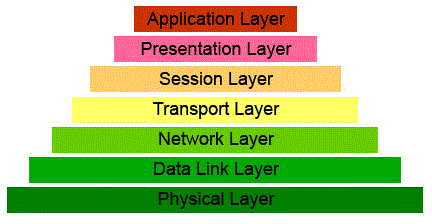
\includegraphics[width=1\textwidth]{figures/layer.JPG}} 
    \caption{osi layer.} 
    \label{layer} 
    \end{figure}
    
 Seperangkat aturan formal yang mendeskripsikan bagaimana cara mentransfer data, terutama dalam jaringan. Protocol level bawah
 mengobservasi standar elektrikal dan fisikal, perintah bit dan byte, pendeteksian transmisi dan kesalahan, serta koreksi terhadap 
 aliran bit. Protocol level atas berkaitan dengan pemformatan data, meliputi sintax pesan, terminal dari dialog computer, susunan 
 karakter, urutan pesan, dan lain-lain.
 
 Ketika data ditransmisikan diantara dua atau lebih peralatan, diperlukan sesuatu yang dapat menjaga control agar data tetap utuh, yaitu 
 suatu deskripsi formal mengenai pesan dan aturan yang harus diikuti oleh dua computer yang ingin bertukar pesan. Protocol dapat 
 mendeskripsikan detal dari interface mesin ke mesin level bawah (cara bagaimana dua program mentransfer file melalui internet).
 
 \section{Elemen Penting Protokol}
 \begin{enumerate}
 \item  Syntax, mengacu pada struktur atau format data, yang mana dalam urutan tampilannya memiliki makna tersendiri.
 \item  Semantics, mengacu pada maksud setiap section bit. Dengan kata lain adalah bagaimana bit-bit tersebut terpola untuk dapat 
 diterjemahkan.
 \item  Timing, mengacu pada 2 karakteristik, yakni kapan data harus dikirm dan seberapa cepat data tersebut dikirim.
 \end{enumerate}

 
 \section{Pengertian Protokol}
Protokol merupakan aturan dalam melakukan pengiriman data (berupa blok-blok data) dari sebuah node jaringan ke node jaringan lain.
Protokol merupakan sarana komunikasi antara mesin melalui jaringan yang terstandarisasi. Protokol mengizinkan data untuk ambil bagian 
dalam transmisi kilat, kemudian ditransmisikan, lalu dikumpulkan kembali sesuai arah dengan perintah yang benar. 
Protokol digunakan untuk mendeteksi kesalahan, tipe kompresi, dan bagaimana receiver (penerima) mengindikasikan bahwa pesan telah 
diterima. 
Protokol dapat mendeskripsikan detail level bawah dari interface machine to machine atau pertukaran level atas antara program alokasi. 
Protokol level bawah meliputi observasi terhadap standar elektrik dan fisik, perintah bit dan byte, pendeteksian transmisi dan 
kesalahan, dan koreksi aliran bit. 
Protokol level atas berkaitan dengan pemformatan data, meliputi sintaks pesan, dialog dari terminal ke komputer, dan pengurutan pesan. 

Protocol merupakan seperangkat aturan komunikasi dimana dalam sebuah hubungan telekomunikasi dapat digunakan untuk menerima sinyal. 
Dalam  koneksi telekomunikasi tersebut protocol dapat  koita bagi menjadi 7 level. Salah satunya yaitu hardware protocol telepon dan 
berupa end point dalam sebuah program komunikasi dalam computer yang sama atau memiliki lokasi yang berbeda-beda. Jadi kedua end point 
tersebut harus dapat mengenali satu sama lain dan mengobservasi protocol.

 \section{Jenis-Jenis Protokol}
Protokol jaringan adalah berbagai protokol yang terdapat dari lapisan  teratas sampai terbawah yang ada dalam sederetan protocol.
Di pandang dari sudut komunikasi data,ada beberapa protokol yang banyak digunakan pada jaringan computer, di antaranya:

 \subsection{TCP/IP}
TCP/IP merupakan protokol standar pada jaringan internet yang tidak tergantung pada jenis computer yang digunakan.
Barangkali perlu dicatat bahwa TCP/IP adalah perlengkapan standar pada sistem operasi Unix dan turunannya.
Saat ini mesin novell,SUN maupun Machintosh sudah dilengkapi protokol standar TCP/IP ini.

Protocol adalah spesifikasi forma yang mendefenisikan prosedur-prosedur yang harus diikuti ketika mengirim dan menerima data (Wermer, 
1996). Protocol mendefenisikan jenis, waktu, urutan dan pengecekan kesalahan yang digunakan dalam jaringan. Transmission control 
protocol/internet protocol (TCP/IP) merupakan protocol untuk mengirim data antar computer pada jaringan. Protocol ini merupakan protocol 
yang digunakan untuk akses internet dan digunakan untuk komunikasi lobal. TCP/IP terdiri atas dua protocol yang terpisah. TCP/IP 
menggunakan pendekatan lapisan (layer) pada saat membangun protocol ini. Dengan adanya pendekatan berlapis ini memungkinkan dibangunnya 
beberaa layanan kecil untuk tugas-tugas khusus.

TCP/IP terdiri dari lima layer, yaitu :
\begin{enumerate}
\item   Layer Application, di dalam layer ini aplikasi seperti FTP, Telnet, SMTP, dan NFS dilaksanakan.
\item   Layer Transport, di dalam layer ini TCP dan UDP menambah data transport ke paket dan melewatkannya ke layer Internet.
\item    Layer Internet, Layer ini mengambil paket dari layer transport dan menambahkah informasi alamat sebelum mengirimkankannya ke layer network interface.
\item     Layer Network Interface, di dalam layer ini data dikirim ke layer physical melalui device jaringan.
\item     Layer Physical, layer ini merupakan system kabel yang digunakan untuk proses mengirim dan menerima data.
\end{enumerate}

\begin{table} [h]
\begin {tabular} {|cc|}
\hline
Lapisan Model OSI & \\
\hline
Application atau Presentation & \\
\hline
Session & \\
\hline
Transport & \\
\hline
Network & \\
\hline
Data Link atau Physical & \\
\hline
\end{tabular}
\end{table} 
  
 \subsection{UDP(User Datagram Protocol)}
UDP adalah salah satu protokol dari layer transport yang merupakan layer ketiga dalam model TCP/IP Layer.
UDP mengirim paket berupa datagram yang terdiri dari sebuah header kecil dan data pengguna UDP memiliki karakteristik connectionless, 
yaitu pengirim mengirimkan paket secara langsung tanpa membangun koneksi ke server. 
Keunggulan lain dari UDP yaitu fleksibel karena rute pengiriman paket dapat dengan mudah diubah, apabila terjadi antrian pada suatu rute tertentu 
 
 \subsection{SNMP(Simple Network Management Protocol)}
SNMP adalah sebuah protokol aplikasi pada jaringan TCP/IP yang menangani manajemen jaringan. 
Protokol ini didesain sehingga pengguna dapat dengan mudah memantau kondisi jaringan komputer. 
Pemantauan kondisi jaringan dapat dilakukan dengan cara pengumpulan nilai-nilai informasi dari kondisi jaringan secara jarak jauh atau 
menggunakan satu pusat pengamatan.
  
 \subsection{AppleTalk} 
Protokol AppleTalk dibuat oleh sebuah perusahann Apple Computer, digunakan pada jaringan dengan komputer mesin Apple, dipublikasikan 
pada tahun 1985. Teknologi Protokol ini milik Apple. Metode akses LocalTalk berfungsi sebaik Ethernet dan Token Ring. 2 metode yaitu 
Manajemen jaringan AppleTalk dan metode akses LocalTalk telah disatukan ke dalam semua mesin Macintosh dan LaserWriter. Bersama produk 
lainnya dari Apple dan mesin tipe lain, AppleTalk dapat kita aplikasikan  baik di PC, VAX maupun  pada workstation UNIX. Sejak AppleTalk 
diperkenalkan (setelah model OSI), protocol Appletalk merupakan routable protocol yang terkandung dalam sebuah network layer (OSI layer 
3). 

\subsection{IPX/SPX(Internet Packet Exchgange/Sequenced Packet)}  
IPX dan SPX adalah protocol standar pada jaringan Novell Netware,untuk mengatasi masalah internetworking pada jaringan 
PC.Kenyataanya,sering kali IPX dijalankan berkaitan dengan TCP/IP karena menguntungkan.Novell Netware merupakan sistem operasi jaringan 
komputeryang dirancang untuk mengaitkan PC ke dalam jaringan antar-PC,yangdapat membuat resource harrdisk dari server dapat digunakan 
bersama.Hubungan antar-client menjadi transparan(antara yang satu dengan lainnya).

Pada tahun 1980-an hingga permulaan tahun 1990-an,sistem operasi ini menguasai hamper seluruh pasaran jaringan computer.
Paket Internetnetwork Packet Exchange(IPX) alamat jaringan dan dapat melakukan pengaturan(route dari satu jaringan ke jaringan 
lain.Sebuah paket IPX terkadang dapat terlewatkan ketika terjadi crossing network, sehingga IPX tidak menjamin pengiriman pesan akan 
terselesaikan. Salah satu dari aplikasi yang tersedia adalah control yang berarti prttokol SPX NetWare harus digunakan. Protokol IPX ini 
berjalan pada layer 3 dan 4 dari model OSI.

AppleTalk Filling Protocol (AFP) adalah sebuah protocol yang digunakan untuk mengatur penerimaan file dan pengiriman file dari komputer 
Apple.
Zone Information Protocol (ZIP) merupakan sebuah  protocol yang digunakan  untuk mengatur sebuah  daerah (zone) yang dibuat  oleh 
jaringan AppleTalk. Zip berfungsi untuk memetakan nomor network ke suatu zone.
Routing Table Maintenance Protokol (RTMP) adalah sebuah  protocol yang digunakan untuk  routing bagi AppleTalk yang berjenis distance 
vector.
Name Binding Protokol (NBP) dapat kita gunakan untuk mengadakan translasi suatu nama dari alamat AppleTalk seperti DNS di TCP/IP).

\subsection{Voice Over Internet Protocol(VoIP)}
Voice Over Internet Protocol merupakan suatu teknologi yang dapat mengirimkan paket suara melalui jaringan Internet Protocol . Jaringan 
Internet Protocol (IP) ini  sendiri merupakan jaringan komunikasi data yang berbasis packet-switch, sehingga dalam berkomunikasi 
menggunakan protocol VoIP berarti menggunakan jaringan internet untuk melakukan komunikasi. Protocol ini juga sering disebut Ip 
Telephony, Internet Tellephony atau Digital Phone.

Pada teknologi VoIP memerlukan protocol agar bisa saling berhubungan dan berkomunikasi, beberapa protocol yang dapat digunakan dalam 
membangun suatu jaringan VoIP adalah protocol H.323 dan Session initiation Protocol (SIP). Pada dasarnya kedua protocol tersebut 
mempunyai peranan yang sangat penting dalam membangun komunikasi menggunakan VoIP. Kualitas suara pada VoIP sangat dipengaruhi oleh 
beberapa parameter, diantaranya adalah bandwidth, delay, filter dan packet loss.

Konsep cara kerja VoIP yaitu dengan melakukan pengiriman sebuah sinyal secara digital, sebelum proses transmisi (pengiriman) dilakukan 
data yang berupa sinyal analog akan dikonversikan terlebih dahulu dengan ADC (Analog to Digital Converter) menjadi bentuk data digital. 
Setelah proses konversi dilakukan data digital akan ditransmisikan ke sumber tujuan.Setelah sampai, data sinyal digital tersebut akan 
dikonversi kembali menjadi data sinyal analog dengan DAC (Digital to Analog Converter) sehingga dapat diterima oleh sumber tujuan 
sesuai dengan data sinyal yang ditransmisikan.

Ada empat komponen pada VoIP yang pertama user agent, merupakan suatu komponen yang digunakan olah pengguna untuk memulai dan menerima 
suatu sesi komunikasi Dalam VoIP. Yang kedua Proxy, merupakan aplikasi server yang mengatur jaringan VoIP. Kemudian protocol, protocol 
merupakan aturan komunikasi yang terjadi Antara user agent dengan proxy. Yang terakhir Codec, codec teknologi yang mempaketkan data 
voice kedalam format lain sehingga menjadi lebih teratur dan mudah dipaketkan.

\subsection{NetBIOS}
NetBIOS digunakan dalam Microsoft Work Group dengan metode peer to peer. Protockol NetBIOS memberikan layanan pada session layer dan 
transport layer (layer 4 dan 5 model OSI). NetBIOS tidak menyediakan format frame untuk kelebihan transmisi jaringan dikarenakan adanya 
berbagai macam perbedaan implementasi NetBIOS yang terjadi. Sebagai contoh, Artisoft LANtastic menggunakan sebuah versi dari NetBIOS 
untuk transmisi antara client dan server. Format frame disusun di NetBEUI, yang digunakan pada semua system operasi Windows yang 
mendukung jaringan.

\subsection{SNA (Systems Network Architecture)}
SNA diperkenalkan pada tahun 1974. Dulunya adalah arsitektur yang terpusat dengan sebuah host komputer dan mengatur banyak terminal. 
SNA mengalami banyak pengembangan,seperti APPN dan APPX(LU 6.2), yang telah mengadaptasi SNA ke dalam komunikasi peer to peer dalam 
lingkungan komputer terdistribusi. SNA Layers diterapkan dilapisan paling bawah yang mengirim paket dari satu stasiun ke stasiun yang 
lain. Lapisan ini merupakan kumpulan beberapa protocol. Walaupun SNA banyak mempengaruhi model OSI, namun ada beberapa perbedaan dalam 
implementasinya.

\subsection{ICMP(Internet Control Message Protocol)}
ICMP merupakan protokol yang digunakan untuk melakukan tes koneksi dari sebuah host ke host yang lain.
ICMP melakukan tes koneksi dengan mengirimkan sebuah request packet ke host tujuan dengan menggunakan IP address.
ICMP merupakan protocol pesan pada TCP/IP. ICMP menyediakan pesan control dan error yang digunakan oleh ping dan traceroute yang bekerja pada layer jaringan.

\subsection{SNMP(Simple Network Management Protocol)
SNMP adalah sebuah protocol yang kita pakai untuk  dapat memantau dan mengontrol jaringan dari tempat lain(jauh). Data dilewatkan dari 
SNMP agent yaitu hardware atau software yang melaporkan suatu aktivitas/proses kepada beberapa perangkat jaringan lainnya seperti hub, 
router, maupun bridge, .Monitoring ini dapat kita  dilakukan melalui console dari workstation. Agent mengembalikan informasi yang 
terdapat pada MIB (management information Base) dimana merupakan sebuah struktur data yang menggambarkan data apa saja yang kita 
dapatkan  dari perangkat dan apa  saja yang dapat dikontrol(dimatikan,dihidupkan,dall).

\subsection{SLIP (Serial Line IP)}
Dalam sebuah data link protocol untuk akses ke jaringan TCP/IP. Biasanya digunakan untuk mendapatkan akses internet.SLIP mengirimkan 
paket IP melalui serial link (dial up atau private line). AX.25 adalah turunan dari protocol x.25 akan tetapi digunakan sebagai protocol 
penghubung dalam jaringan paket radio. Selain itu sebetulnya masih ada kelurga protocol yang lain, seperti yang dikembangkan oleh 
OSI/ISO: X.25/X.75/X.400 yang juga mulia digunakan oleh beberapa institusi.

UUCP (Unix-to-Unix Copy Program), pada mulanya untuk mengirimkan file antarmesin Unix. File-file itu dapat berupa surat elektronik (e-
mail) maupun konferensi elektronik (news). Solusi ini baik untuk pengembangan jangka panjang sebuah jaringan computer, akan tetapi dapat 
digunakan untuk solusi sementara yang bersifat darurat. Sayang segala informasi tentang protocol ini harus dibeli keke ISO. Hal ini 
dapat berkembang ISO/OSI tersendat, tidak seperti TCP/IP.

\subsection{FTP (File Transfer Protocol)}
FTP adalah sebuah protokol Internet yang berjalan di dalam lapisan aplikasi yang merupakan standar untuk pentransferan berkas antar 
mesin-mesin dalam sebuah Internetwork. 
FTP didefinisikan sebagai sebuah protokol untuk mengirim dan menerima file antara host (dalam Advanced Research Project Agency Network 
(ARPANET). 
Fungsi utama dari FTP adalah mengirim dan menerima file dengan efisien dan handal antara host dan mengijinkan penggunaan yang nyaman 
dari kemampuan untuk penyimpanan file secara remote.

\subsection{elemen yang terdapat pada protokol}
Elemen penting protocol adalah syntax,semantics,dan timing.
-Yang pertama Syntax maksudnya yaitu dipusatkan pada struktur atau format data, yang mana dalam urutan tampilannya memiliki makna 
tersendiri. Sebagai contoh sebuah protocol sederhana akan memilki urutan pada 8 bit pertama sebagai alamat pengirim,dan bit selanjutnya 
itu adalah informasi tersendiri. 
-Yang kedua yaitu semantic yang mengacu pada maksud setiap section pada bit dapat dikatakan bahwa beberapa bit bit tersebut terpola  
sehingga bit bit tersebut dapat  kita diterjemahkan.
-Yang ketiga yaitu timing, timing lebih dipusatkan kepada 2 karakteristik,yaitu  kapan suatu data tersebut seharusnya dikirimkan dan 
yang kedua seberapa cepat data tersebut dapat kita kirim.

\end{document}


\chapter[Arsitektur Client Server]
{Arsitektur Client Server}

\section{ArsitekturClientServer}
    Pada Table \ref{table} terdapat beberapa model Arsitektur yang terdapat didalam Sebuah Web Service. 
Arsitektur Client Server merupakan  sebuah model yang membedakan kinerja koputer sebagai client dan server. 
Arsitektur akan menyesuaikan komputer sebagai server dan server akan melayani client yang terhubung kedalam sebuah jaringan.
Server dapat melayani berbagai file server, sebuah printer, bahkan jalur komunikasi.
Client tidak dapat berfungsi sebagai server akan tetapi server dapat berfungsi menjadi client yang dinamakan `server non-dedicated'.
Kerjanga Arsitektur ini sangatlah simpel yaitu server akan menunggu client membuat permintaan dan server akan memproses serta
akan memberikan hasilnya kepada client. Berbeda dengan client, tugas client akan mengirimkan sebuah permintaan kepada server, lalu
client akan menunggu respon yang diberikan oleh server.

\begin{table}[ht]
\caption{Model Arsitektur Client\-Server}
\centering
\begin{tabular}{ccc}
\hline
1\-Tier&2\-Tier&3\-Tier\\
\hline
Stand\-Alone&Client\-Server&Multi\-Tier\\
\hline
\end{tabular}
\label{table}
\end{table}

\section{ArsitekturWebService}
Memiliki 3 entitas yaitu :
\begin{enumerate}
\item Service Provider adalah penyedia layanan untuk meyediakan layanan serta mengolah registry supaya layanan-layanan tersebut tersedia.
\item Service Registry adalah daftar layanan sebagai lokasi pusat yang mendeskripsikan semua layanan yang telah melakukan register.
\item Service Requester merupakan layanan yang berfungsi mencari dan menemukan layanan yang dibutuhkan serta menggunakan layanan tersebut.
\end{enumerate}

\section{Penerapan XML di WebService}
Pada layanan web ialah suatu konsep yang baru dalam sistem yang terdistribusi melalui web yang menggunakan teknologi xml dengan 
menggunakan protokol yang standar SOAP dan HTTP. Dengan menggunakan layanan web sangat dapat mendukung sistem yang terdistribusi 
yang telah memiliki insfratuktur yang berbeda pula, karena kini layanan web telah menggunakan xml maka dari itu teknologi ini telah dapat 
mendukung dari berbagai platform yang ada pada sistem maupun aplikasi.

\section{Peran SOAP di WebSevice}
Pesan berbasis XML melalui jaringan komputer pada program yang berjalan pada sistem operasi, berkomunikasi pada program Operating 
System yang sama maupun berbeda. 
HTTP dan XML sebagai mekanisme pertukaran data, SOAP dapat berkomunikasi dengan berbagai aplikasi meskipun perbedaan sistem operasi. 
Jadi, SOAP pada web service merupakan aplikasi pesan yang tergantung pada skema XML, sebagai protokol pemaketan pesan-pesan yang digunakan 
secara bersama oleh aplikasi penggunanya adalah peranan SOAP.

\section{Arsitektur Server}
Arsitektur client/server menggunakan LAN untuk menjalankan personal komputer, Modul LAN dan DBMS mengendalikan, mengamankan secara 
bersamaan dan merupakan query untuk support akses dari beberapa pengguna dalam menyambungkan database.
Arsitektur client/memiliki tiga komponen antaranya :
\begin{enumerate}
\item Presentation Logic, menangani memformat dan mempresenting data pada pengguna.
\item Processing Logic, komponen ini menangani logika data pemrosesan. Proses data logic merupakan aktifitas memvalidasi data, 
mengindentifikasi proses error pada data.
\item Storage Logic, menangani penyimpanan, perbaikan data dari alat penyimpanan yang bekerja dengan aplikasi tersebut.
\end{enumerate}

\section{Arsitektur Client}
Komponen Client sering disebut front-end, sebaliknya komponen server disebut sebagai back-end. 
Komponen Client dijalankan dari sebuah aplikasi dalam workstation dan menerima masukan data dari pengguna, data yang disiapkan 
dimasukkan oleh pengguna dengan menggunakan teknologi pemroresan lalu mengirimkannya pada komponen server diatas. 
Pada umumnya dalam bentuk request terhadap beberapa service yang dimiliki oleh server. 
Server akan menerima request dari Client dan langsung memprosesnya lalu mengembalikan hasil proses tersebut pada Client dalam sistem 
server pemrosesan pada DBMS.

\section{Komponen Client-Server}
Dari sisi server bertugas melayani client dalam hal memberikan data yang diminta oleh client.
Lalu, model 2-tier server meyediakan sebuah Stored procedure, Triggers, Query. 
Mengapa menggunakan MySQL dari pada MS SQL server yang lebih kompatibel dengan Visual Basic? Karena, aplikasi MS SQL bersifat komersial tentu 
anda harus membelinya. Sebaliknya dengan MySQL server bersifat gratis yang mudah didapatkan serta banyak yang menggunakannya. 
Sedangkan dari sisi Client bertugas menyediakan interface untuk pengguna dalam mengoperasikan pada database. Interface dapat dibuat dengan 
menggunakan bahasa pemrograman yang sudah kita ketahui, contoh seperti bahasa pemrograman pada Visual Studio 
\(VB, C\# dan Visual C\|++|\), Java, Delpi dan lain-lain. 
Interface menyediakan tampilan untuk memudahkan pengguna dalam mengedit, mendelete serta menampilkan data yang ada di DBMS komputer server 
ke komputer client.

\section{Konsep Client-Server}
Clien-Server ialah komunikasi antara 2 atau lebih pada komputer yang melakukan pembagian tugas masing-masing komputer. 
Client memiliki beberapa tugas yaitu : input, update, delete, dan dapat menampilkan data sebuah database. 
Sedangkan Server bertugas untuk menyediakan pelayanan untuk melakukan managemen, yaitu : 
menyimpan \& mengolah database. 
Aplikasi Client-server merupakan jawaban atas berkembangnya teknologi informasi, 
di mana suatu perusahaan memiliki banyak departemen dan harus terhubung satu sama lain dalam melakukan akses data.

\section{Keuntungan Penerapan Client-Server Web Service}
Web Service bisa digunakan untuk alternatif dalam pengembangan Aplikasi n-tier, yang mana dapat dipisahkan
antara Database, aplikasi dan Klien. 

dalam penerapan n-tier ke web service, untuk logika aplikasi dapat diterapkan dengan web services
sehingga disisi klient tidak direpotkan dengan instalasi beberapa layer seperti halnya corba atau sejenisnya.
dengan menggunakan web service, method atau function yang developer buat dapat digunakan berulang - ulang bahkan
untuk keperluan aplikasi yang berbeda (penggunaan kembali function). penerapan yang lebih jauh dari web service adalah SOA dan SOAP

\section{Contoh penerapan Client-server Web Service}

\subsection{Pencarian Objek Wisata Berbasis Android}
Pengimplementasian dari Web Service didalam sebuah perangkat android untuk memproses
dalam pencarian objek wisata menggunakan android, proses yang terjadi didalamnya adalah :

\begin{enumerate}
    \item Pilihan objek wisata berdasarkan kategori yang diinginkan.
    \item Fitur explore atau pencarian objek wisata berdasarkan kriteria yang diinginkan
    \item Review dan detail mengenai sebuah objek wisata.
    \item Fitur direksi untuk menunjukkan jalan menuju lokasi wisata yang dipilih dengan memanfaatkan google maupun
    \item Add Location atau fitur menambahkan lokasi objek wisata yang dikunjungi
\end{enumerate}

\subsection{Layanan Informasi Pekerjaan Online}
Pada zaman sekarang ini tingkat kebutuhan hidup manusia sudah sangat tinggi sehingga mendorong orang - orang
untuk mencari pekerjaan yang layak agar dapat menghidupi dirinya sendiri dan keluarganya. sehingga 
layanan informasi untuk pencarian pekerjaan secara online dibutuhkan, namun semakin marak juga kebocoran
data dari para pelamar. sehingga dipergunakanlah Web Service yang juga dalam penerapannya menggunakan
implemetasi Client-Server, cara kerja sistem yang ingin dibuat adalah sebagai berikut :

\begin{enumerate}
    \item tamu yang berkunjung untuk mencari pekerjaan 
    \begin{enumerate}
        \item mendapatkan lima lowongan pekerjaan terakhir untuk setiap kategori
        \item mencari lowongan kerja berdasarkan kriteria tertentu.
    \end{enumerate}

    \item Anggota pencari kerja

    \begin{enumerate}
        \item memasukan CV pribadi
        \item memasukan data minat pekerjaan yang diminati
        \item mendapatkan email berisi lowongan kerja yang sesuai data minat pekerajaan
    \end{enumerate}
\end{enumerate}

\subsection{Arsitektur Layanan Perawatan Medis Mobile}
Pada penerapan arsitektur client-server yang satu ini bergerak di bidang kesehatan, dimana Pasien dapat melakukan check kesehatan
walau terpantau jarak yang jauh sekalipun. Dengan menggunakan sebuah telepon selular dapat mencakup kegiatan pengecekan kesehatan.
Dimana Layanan yang diberikan oleh aplikasi ini adalah :
\begin{enumerate}
    \item layanan kesehatan yang menamplkan dengan penggunaan sensor
    \item menjamin dalam sistem keamanannya karena penggunaan software yang dinamik serta dapat diupgrade dengan terpaut data klinik
    \item remote registrasi dimana data yang didapat oleh pasien didapat melalui proses upload dan download yang dilakukan oleh sensor
\end{enumerate}

\subsection{E-LEARNING OLAT} 
Clustering basis data merupakan kumpulan server yang dikonfigurasikan oleh suatu perangkat lunak DBMS sehingga menjadi satu kesatuan sistem 
untuk menangani manajemen basis data \(Anonim, Postgresql, 2008\). Menurut Vishal Batra \(2008\), salah satu manfaat dari clustering basis data 
adalah terjaganya aspek `Availibility', artinya akses dari client pada jumlah tertentu secara simultan akan dijamin dapat dilayani oleh 
server-server dalam lingkungan cluster. Keterjaminan layanan akan menyebabkan kelancaran akses client.

\subsection{Sistem Layanan Pariwisata Terpadu}
Penerapan Arsitektur Client-Server ke Web Service dapat disimpulkan dari hasil pengembangan aplikasi ini, seperti yang tertera bahwa tingkat Pariwisata
dari turis lokal Maupun turis mancanegara sangat tinggi sehingga menuntut sebuah agen pariwisata untuk terus meningkatkan pelayanannya. salah satunya dengan
mengadakan sebuah Aplikasi yang berbasis Web, bukan hanya berbasis web saja namun juga memiliki keamanan akan data user yang dimiliki pengguna dan juga kemudahan
dalam penggunaan aplikasi tersebut. sehingga penerapan Web Service juga berperan penting dalam hal ini, hasil yang di keluarkan dari penerapan Web Service dan juga
Arsitektur Client-Server dari Aplikasi ini adalah :

\begin{enumerate}
    \item dalam pengembangan Aplikasi ini digunakan sistem Arsitektur Multi-Tier
    \item dalam melakukan pengembangannya Web Service sangat mudah untuk pengembangan selanjutnya
    \item Integrasi antara Web-Service dari Aplikasi ini dengan Aplikasi Web-Service `Kurs' sudah terbangun, sehingga ketersediaan akan Pelayanan yang diminta akan lebih dimudahkan
    \item dapat berjalan dengan lancar walaupun dengan penggunaan Sistem Operasi yang berbeda
\end{enumerate}

\subsection{Hubungan Kualitas Jasa, Kepuasan Nasabah dan Intensi Pembelian Ulang}
Penelitian ini dirancang untuk menguji korelasi antara kualitas layanan, kepuasan pelanggan dan niat pembelian. Secara rinci penelitian 
ini meneliti tiga korelasi, yaitu diantaranya :

\begin{enumerate}
\item kualitas layanan dan niat pembelian  
\item kepuasan pelanggan
\item kualitas layanan dan kepuasan pelanggan
\end{enumerate}

Ada tiga hipotesis yang diajukan di sini, yaitu :
\begin{enumerate}
\item kualitas layanan memiliki pengaruh signifikan terhadap niat membeli 
\item kepuasan pelanggan memiliki pengaruh signifikan terhadap niat membeli
\item kualitas layanan memiliki pengaruh signifikan terhadap kepuasan pelanggan 
\end{enumerate}

\section{Arsitektur Database Server}
Dalam Arsitekture Client Server juga membutuhkan atau menggunakan sebuah Database, terutama di dalam server ada yang
dinamakan dengan Arsitekture Database Server yaitu dimana Client akan bertanggung jawab dalam pengelolaan antar muka pemakai
sedangkan Database Server akan bertanggung jawab dengan pada penyimpanan, pengaksesan, serta pemrosesan database.
Di dalam Database Server ini memiliki sebuah kemampuan dalam pemrosesan yang cukup tinggi sehingga beban dalam jaringan akan 
menjadi berkurang. Database Server ini termasuk kedalam two-tier architecture.

\section{Penggunaan Teknologi internet dalam Dunia Bisnis}
Pemasaran internet ada 2 metode yaitu, push dan pull marketing. Keuntungan yang dapat diperoleh dari internet ialah komunikasi 
global dan interaktif; yang menyediakan suatu informasi dan pelayanan sesuai dengan kebutuhan konsumen; meningkatkan kerjasama; 
kemudian memungkinkan bagi pengguna untuk membuka pasar,produk, atau pelayanan baru; serta mengintegrasikan aktivitas secara online. 
Pembayaran transaksi electronic commerce diatur oleh Secure Socket Layer yang dikembangkan menjadi Secure Electronic Transaction

\section{Model Arsitektur Client Server}
Dalam Arsitektur Client Server terdapat 3 model arsitektur yaitu :

\begin{enumerate}
	\item Arsitektur Single-tier atau satu lapis
	\item Arsitektur Two-tier atau dua lapis
	\item Arsitektur Three-tier atau tiga lapis
\end{enumerate}

\subsection{Arsitektur Single-tier atau satu lapis}
Pada gambar \ref{Stand} dijelaskan tentang Arsitektur Single-tier ini merupakan model yang paling sederhana sehingga sangat mudah digunakan oleh pengguna atau user.
Arsitekur Single-tier ini adalah model aristektur yang paling sedikit memiliki alternatif, sehingga dalam Arsitektur Single-tier ini
memiliki kelemahan yaitu seperti kurang aman dan kurang memiliki skalabilitas.

\begin{figure}[h]
    \centerline{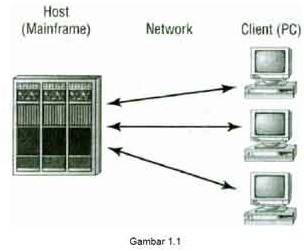
\includegraphics{figures/2modelstandalone.JPG}}
    \caption{Model Arsitektur 1 Tier atau Stand Alone}
    \label{Stand}
\end{figure}

\subsection{Arsitektur Two-tier atau dua lapis}
Pada gambar \ref{Tier2} dijelaskan bahwa dalam Arsitektur Two-tier ini dapat dibagi dua dalam pengelolaan informasinya, yaitu dalam UI `User Interface` lingkungan dan dalam
lingkungan server manajemen databasenya. Dibandingkan dengan Arsitektur Single-tier, Arsitekur Two-tier ini mimiliki tingkat
keamanan yang cukup tinggi serta teratur. Arsitektur Two-tier ini memiliki database terpisah pada setiap komputer sehingga dalam
Arsitektur Two-tier ini dapat meningkatkan kinerja dalam keseluruhan situs. Kelemahan yang dimiliki oleh Arsitektur Two-tier ini
adalah tentunya memiliki biaya yang cukup mahal, tidak adanya pembaharuan kode, serta arsitekturnya yang kompleks.

\begin{figure}[h]
    \centerline{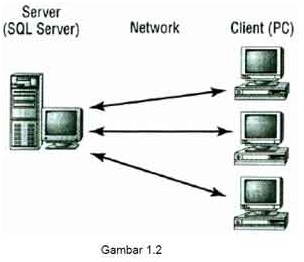
\includegraphics{figures/2model2tier.JPG}}
    \caption{Model Arsitektur 2 Tier atau Client-Server}
    \label{Tier2}
\end{figure}

\subsection{Arsitektur Three-tier atau tiga lapis}
    Pada gambar \ref{Tier3} dijelaskan bahwasanya Awal muncul dari Arsitektur Three-tier ini dikarenakan 
di Arsitektur sebelumnya memiliki cukup banyak kelemahannya, maka dari itu Arsitektur Three-tier ini akan mengatasi kelemahan yang 
dimiliki oleh Arsitektur Two-tier. Kelebihan dari Arsitektur Three-tier ini yaitu dia memiliki skala yang besar, dan memiliki daya 
transfer informasi antara web server dengan server database optimal. tetapi Arsitektur Three-tier ini juga mempunyai kelemahan atau dengan jumlah tiga lapis maka biaya yang dikeluarkan cukup mahal. Ada beberapa bagian dari arsitektur Three-tier ini yaitu 

	\begin{enumerate}
		\item Presentasion Layer yaitu sebuah layer yang berada di posisi puncak atau posisi tertinggi biasanya juga sering disebut
		         sebagai User Interface. Presentasion Layer ini berfungsi untuk menerjemahkan tugas dan hasil yang telah dikerjakan
		         oleh layer - layer sebelumnya
		\item Logical Layer merupakan koordinat dari sebuah aplikasi, serta memproses perintah dari aplikasi, dan membuat
		         keputusan yang logic dan evaluasi serta mengperhitungkan performa, sehingga Logical Layer ini dapat memindahkan
		         serta memproses 2 layer
		\item Data Layer berfungsi sebagai tempat untuk menyimpan sebuah informasi serta mengolah data dan file sistem. Lalu
		         informasi tersebuh akan dikirim ke logical layer dan akan dikembalikan kepada user.
	\end{enumerate}

\begin{figure}[h]
    \centerline{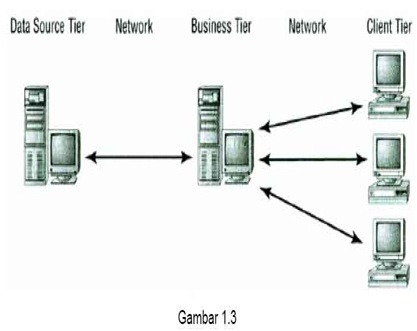
\includegraphics{figures/2model3tier.JPG}}
    \caption{Model Arsitektur Three-Tier atau Multi-Tier}
    \label{Tier3}
\end{figure}

\section{Rest Web Service}
Pada umumnya penemuan yang menyediakan suatu metode dan sistem yang terkomputerisasi untuk memonitori layanan web rest yang termasuk
membangkitkan lagi operasi pemanggilan klien layanan web yang berbasis rest yyang akan digunakan untuk memonitoring aktivitas pada layanan web.
Metode atau sistem komputerisasi yang lebih lanjut mencakup pemantauan aktivitas layanan web dengan melalui suaru panggilan-panggikan dan tanggapan analisis.

\section{Pemrograman Web pada client server}
Saat ini, perkembangan pada aplikasi yang berbasis Web sangat pesat karena memang memiliki beberapa kelebihan dibandingkan aplikasi berbasis deskop. Berikut adalah beberapa contoh kelebihan pada aplikasi yang berbasis web :

\begin{enumerate}
    \item Pada sisi client user, tidak emerlukan proses intalisasi. Jika terjadi perubahan pada aplikasi, client juga tidak perlu repot-repot melakukan proses update karena cukup dilakukan  pada server.
    \item Data disimpan di sisi server, sehingga akses terhadap data dari sisi client user dapat di atur sesuai kebutuhan
    \item Dari sisi client, tidak memerlukan spesifikasi komputer yang besar karena hamper selruh proses aplikasi dilakukan di sisi server
    \item Client user lebih aman dari virus atau gangguan keamanan lainnya karena aplikasi berjalan di atas browser.
\end{enumerate}

\section{Web Service Security}
Pada layanan web keamanannya mengamankan suatau layanan karena pada sifatnya terhubung secara longgar dan penggunaan aksesnya terbuka terutama pada http yang
 dilakukan oleh layanan web dengan menambahkan sekumpulaan keamanan layanan web yang baru. Teruntuk keamanan pada layanan web juga termasuk memiliki konten aplikasi yang dikirim dengan menggunakan platform cdn global. 




    


\chapter[Common Gateway Interface]
{Common Gateway Interface}
%KELOMPOK 4 Blank-On1
%\begin{enumerate}
%\item Andri Fajar Sunandhar
%\item Cokro Edi Prawiro
%\item Fadila
%\item Sandro Samuel Sinaga
%\end{enumerate}



\section{Common Gateway Interface}
CGI merupakan metode yang dipakai untuk mempertukarkan data di antara server dan klien (browser). CGI merupakan sebuah standar dimana program atau script bisa mengirim data kembali ke web server dimana ia diproses, yaitu dengan menggunakan tag HTML standar untuk mendapatkan data dari seseorang, kemudian meneruskannya ke CGI. Selanjutnya CGI melakukan serangkaian aksi terkait data tersebut\cite{prihatmoko2013pengembangan}.



\par CGI adalah interface untuk menjalankan program-program eksternal,dibawah informasi server, biasanya server HTTP (walaupun CGI standar dirancang untuk lintasan-platform yang
menangani semua jenis hardware dan software yang berbeda, windows CGI 1.3 khusus untuk platform microsoft Windows 95/98 dan windows NT). Dengan CGI server bisa
melayani informasi yang tidak ada dalam format yang mudah dibaca oleh client,seperti data yang ada dalam database SQL, dan melakukan gateway antara dua sesuatu yang 
dihasilkan oleh browser client. Seringkali program gateway ini disebut script.

\par Sebuah server web memproses permintaan klien CGI menggunakan skrip atau aplikasi CGI. Sebagai contoh, ketika sebuah database ditanyakan oleh klien, 
server web bertindak sebagai gateway antara database dan klien. Server web mentransmisikan permintaan klien ke aplikasi CGI yang melakukan kueri basis data,
 memformat hasil dan mengembalikan data berformat HTML ke server web. Server web kemudian mentransmisikan data berformat HTML ke klien untuk ditampilkan kepada pengguna.

\par Di server, protokol yang diperluas lebih didukung oleh antarmuka gerbang umum (CGI) yang mengubah komunikasi dari perangkat I / O non-standar ke format yang kompatibel 
dengan transaksi atau program aplikasi data yang dapat dijalankan pada server atau komputer yang dipasangkan ke server. 
Dengan cara ini, CGI memungkinkan pemrosesan perintah kemampuan yang diperluas untuk dipisahkan dari fungsi komunikasi yang dilakukan oleh server.

\par Adapun pengertian lain dari Common Gateway Interface yaitu sekumpulan aturan untuk mengarahkan sebuah server web berkomunikasi dengan software dalam mesin yang sama begitu pula sebaliknya antara software CGI programs dengan web server. Setiap perangkat lunak dapat menjadi perogram CGI dengan syarat software tersebut dapat melakukan input dan output sesuai setandar CGI. CGI menjadi setandar menghubungkan untuk menghubungkan data informasi yang terjadi antara server dan aplikasi, seperti HTTP. Script CGI dapat mengirtimkan data kembali ke web server  dimana CGI diperoses. CGI merupakan interface antara halaman website dengan web server yang menjalankan perogram\cite{aditya2015analisis}.

\begin{figure}[ht]
\centerline{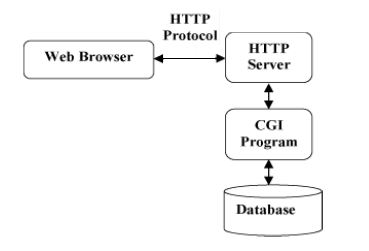
\includegraphics[width=1\textwidth]{figures/1arsitekturCGI.JPG}}

\caption{CGI Arsitektur Diagram} 
\label{1arsitekturCGI}
\end{figure}

Gambar\ref{1arsitekturCGI} menjelaskan bahwa antara HTTP server di pelantarai oleh CGI program dalam mengakses data 
dari database. Jadi jika data yang diminta di batasi atau tidak memiliki hak akses oleh CGI data tersebut tidak dapat di munculkan 
oleh web browser.  Cara untuk memahami perinsip dari (Common Gateway Interface ) CGI, dapat dicoba dengan melakukan click pada suatu URL suatu website.
setelah melakukan hal tersebut browser akan menghubungi HTTP web server dan meminta URL dari website tersebut. Kemudian web server tersebut akan
mengurai (prasing) URL dan akan mencari berkas dari link tersebut, bila ditemukan maka akan diteruskan ke browse, begitu juga sebaliknya jika tidak ada
maka akan diberikan pesan error. lalu web browser akan menampilkan hasilnya, baik url yang tadi diminta maupun pesan error karena URL yang dituju tidak ada. Meski begitu, ada kemungkinan untuk mengatur suatu HTTP server untuk membatasi akses terhadap suatu berkas.
jadi halaman URL yang dituju tidak bisa diakses hal tersebut merupakan fungsi dari CGI script. supaya lebih paham dapat dilihat 
pada arsitektir program CGI.

\par  CGI (Common Gateway Interface) memungkinkan server web memanggil suatu program, lalu mengirimkan data-data spesifik dari pengguna ke program tersebut.
 Hasil proses tadi diterima oleh CGI yang selanjutnya menyerahkannya kepada server web untuk kemudian, yang pada gilirannya akan mengirimkan
informasi tersebut kembali dalam bentuk HTML ke browser web pengguna, Server web kemudian mentransmisikan data berformat HTML ke klien untuk ditampilkan kepada pengguna. \cite{ibrahim2011sistem}.

\section{PHP and Common Gateway Interface interconnections }
Common Gateway Interface is a standard that is used to connect various application programs to web pages. One example of the programming language is PHP. PHP is a software that is open source and can pass across the various platform. Php can be run in 2 ways ie as apache module in web server and also as binary in Common Gateway Interface.This language was created in 1994 by Ramus Lerdoff.  Initially, PHP is a CGI program that is devoted to receiving input through forms displayed in web pages or browser. The PHP code is usually processed by a PHP interpreter which is usually executed as a native web server module or Common Gateway Interface\cite{nahado2015bumbu}.


\section{Security in Common Gateway Interface }
Common Gateway Interface is used to connect WWW (World Wide Web) systems with software or other software on the web server. The presence of the Common Gateway Interface allows connection interactive between the user and also the web server. Common Gateway Interface itself is often used as a mechanism to get information from users through "fill out a form", access the database, or generate dynamic pages. Although in principle the mechanisms in the Common Gateway Interface do not have security holes, programs or scripts created as CGI can have security flaws either created intentionally or unintentionally. That is because CGI program itself is run on the web server to use the web server resources.


\section{The Application of Common Gateway Interface }
CGI is applied to the making of applications involving python language with PHP language. CGI itself is implemented or modified as CGI Fast CGI protocol, where its function in the application is as an interface in other applications to the web server which is an alternative facility to improve its own performance for CGI which is intended for the web server application process which is Apache web server to dynamic language another. Processes and handling from CGI to FastCGI can be demonstrated from the use of this working support facility such as python as the dynamic language used and the fastCGI module for the server to be used on RFC2109 proxy caching.


\section{ Web Database and Common Gateway Interface Interconnections }
The Internet database development platform is adapted for approaches by connecting with or from CGI (Common Gateway Interface). The technical description includes a discussion of the Common Gateway Interface in which CGI functions as an interface for executing information on external programs, under server information, usually HTTP servers (although the Common Gateway Interface standard is designed for path-platforms that handle all different hardware and software.) Using a CGI server can serve information that does not exist in a format that is easy to read by the client, such as in existing data in SQL databases, and performs a gateway between two things generated by the client browser, which is usually the gateway program called scripts.


\section{Honeypot}
Menurut Lance Spitzner Honeypot adalah sumber daya keamanan yang mempunyai nilai jika sistem disusupi atau diserang. Pada dasarnya Honeypot merupakan suatu alat untuk mendapatkan informasi dari penyerang. Honeypot merupakan sistem yang dirancang untuk diperiksa dan diserang.
Honeypot Dionaea merupakan salah satu Honeypot interaksi rendah yang bertujuan menangkap salinan malware berbahaya yang masuk ke dalam sistem. Malware tersebut biasanya ada pada layanan yang ditawarkan dalam jaringan. Dionaea menggunakan Python sebagai bahasa script dan libemu sebagai pemecah kode. Dionaea mendukung Internet Protocol v6 dan Transport Layer Security (TLS)\cite{andros2015implementasi}.

\section{Web Server Gateway Interface (WSGI) }
Salah satu keunggulan yang dijelaskan sebelumnya adalah karena Google App Engine dan Django dirancang untuk menggunakan standar WSGI untuk menjalankan aplikasi.
Django dapat berjalan dengan lingkungan server yang berbeda. Misalnya yang populer Server Apache didukung menggunakan mod python atau mod wsgi.
Juga untuk python maprelational Objectperational mendukung PostgreSQL, MySQL, SQLite dan Oracle.

\par Sebuah server web diatur di atas sistem operasi untuk mengirim permintaan HTTP, tetapi juga bisa melayani file statis seperti gambar, file JavaScript, halaman HTML, dll.
 Itu memproses pesan JSON dengan Flask, yang merupakan kerangka mikro untuk Python yang difokuskan pada kode aplikasi web, Karena server web tidak dapat berkomunikasi
 secara langsung dengan Flask, kami mengimplementasikan Web Server Gateway Interface (WSGI) untuk bertindak sebagai proxy antara server dan Python / Flask.


\chapter{Instalasi PIP dan Contoh Penggunaan}
{Instalasi PIP dan Contoh Penggunaan}
\documentclass[12pt,a4paper]{article} 
\usepackage{graphicx}
\linespread{1.5}
\begin{document}
\title{Instalasi PIP dan Contoh Penggunaan}
\maketitle

\begin{itemize}
\item
Nama Kelompok 1\\
Farid Ariyanto Saputra 1164036\\
Nurgivani Syarifatul Husna 1164050\\
Velariza Alvioletta 1164056\\
Yogi Aditya Saputra 1164060 \\
\end{itemize}

\section{Python}
\subsection{Pengertian Python}
Python merupakan salah satu Bahasa pemrograman yang bersifat open source yang tertafsir oleh typing yang dinamis dan kuat. Python juga memiliki banyak library, seperti struktur data, files, dan jaringan. Bahasa pemrograman python juga banyak digunakan untuk berbagai keperluan, contohnya komputasi ilmiah, system administrasi, dan pengembangan web. Selain itu pula, keuntungan Bahasa pemrograman python yakni memiliki alat simulasi python gratis.
\subsection{Pengertian Python}
Python adalah suatu bahasa pemrograman yang bisa dikatakan bahasa pemrograman jaman sekarang, karena usianya sangat muda namun sudah banyak digunakan oleh programmer. Phyton dapat mendukung dalam membangun aplikasi berbasis desktop, web, mobile maupun lainnya. Untuk membangun sebuah aplikasi, bahasa pemrograman ini juga bisa digunakan menggunakan framework maupun tanpa framework. Namun, apabila tidak menggunakan framework akan membutuhkan waktu yang lama dalam tahap membangun aplikasi, begitu juga sebaliknya apabila menggunakan framework pembangunan aplikasi akan menjadi lebih cepat dan terstruktur, biasanya framework yang digunakan adalah Django, dimana disana terlah tersedia komponen seperti models, templates, views, forms, dan admin interface.
\subsection{Pengertian Python}
Python merupakan sebuah bahasa dalam pemrograman yang dibuat oleh Guido Van Rossum dan populer sebagai sebuah bahasa pemrograman berbasis Web. Python dikenal sebagai sebuah bahasa yang menggabungkan kapabilitas, kemahiran, dengan sintaksis kode yang jelas. Mengambil dari pengertian wikipedia, Python merupakan sebuah bahasa pemrograman interpretatif yang bisa digunakan dalam berbagai macam program web dengan filosofi perancangan yang berfokus ada tingkat keterbacaan kode.
\subsection{Pengertian Python}
Phyton merupakan salah satu Bahasa pemrograman kelas atas serta memiliki sifat intrepeter, object oriented, serta interaktif serta dapat berjalan pada sistem operasi seperti UNIX, MAC, Windows maupun platfrom lain. Karena Python merupakan bahasa pemrograman kelas tinggi, python dapat di kombinasikan dalam penggunaan tata kalimat dengan modul-modul yang telah siap pakai serta struktur data yang lebih efisien.
\subsubsection{Perbedaan Pyhton 2 dan Pyhton 3}
Berikut adalah tabel \ref{table:perbedaan} perbedaan python 2 dan python 3, yaitu :
\begin{table}[h]
\caption{Perbedaan Pyhton 2 dan Pyhton 3}
\centering
\begin{tabular}{ccc}
\hline
 &Pyhton 2&Pyhton 3\\
\hline
versi pyhton&python --version&pyhton3 --version\\
publikasikan&2000&2008\\
Fokus&Lebih Transaparan dan inklusif &perapian pada codebase\\
&untuk pengembangan&dan menghapus duplikasi\\
Coding&print "coba"  &print ("coba")\\
&tidak harus menggunakan tanda kurung& harus menggunakan tanda kurung\\
\end{tabular}
\label{table:perbedaan}
\end{table}

\section{PIP}
\subsection{Pengertian PIP}
PIP yang memiliki kepanjangan dari Pyhton Index Packaging. PIP itu sendiri adalah sebuah app store atau biasa disebut package manager yang biasa digunakan untuk mencari, mengunduh, menginstal serta mengelola package atau modules yang biasa ditemukan di PyPI ( Pyhton Package Index ). Dimana PyPI adalah sebuah library perangkat lunak untuk Bahasa pemrograman Pyhton.
\subsection{Pengertian PIP}
PIP merupakan singkatan dari python index packaging. PIP adalah sebuah aplikasi manajemen package yang biasa digunakan untuk menginstall dan mengelola package yang telah ditulis oleh python. Untuk menemukan packagenya, kita bisa mencari di situs Python Package Index (PyPI). Ada kurang lebih 134443 package dalam python yang bisa diinstall melalui PyPI.
\subsection{Pengertian PIP}
PIP (python index packaging) merupakan Package Management System yang biasanya digunakan untuk mengunduh dan mengelola package Python. Banyak sekali package yang bisa di temukan di PyPI. 
PIP bisa langsung digunakan di Python versi 2.7.9 dan versi 3 namun apabila menggunakan versi dibawahnya harus melakukan instalasi terlebih dahulu. 
Pip juga sebuah sistem untuk memeriksa perilaku sistem terdistribusi secara otomatis terhadap harapan programmer tentang sistem. Pip mengklasifikasikan perilaku sistem valid atau tidak valid, mengelompokkan perilaku ke dalam set yang dapat dipikirkan, dan menyajikan perilaku keseluruhan dalam beberapa bentuk yang sesuai untuk menemukan atau memverifikasi kebenaran perilaku sistem.
\subsection{Pengertian PIP}
PIP merupakan singkatan dari python index packaging yang merupakan package management sistem yang sering kali di gunakan untuk mengelola package python. Packages python dipasang dengan manajer paket pip, yang termasuk dalam semua lingkungan virtual. seperti sesi prompt perintah python akan memanggil versi alat ini daripada milik virtual enviroment yang diaktifkan.

\section{Cara Instalasi PIP}
\subsection{Instalasi di Windows}
Berikut adalah cara menginstall PIP atau Python Index Packaging. \\
1.	Kunjungi web resmi https://pip.pypa.io/en/stable/installing/ untuk mendownload dan melihat cara instalasi di windows.\\
2.	Download get-pip.py dari web tersebut. \\
3.	Buka Python.exe atau buka CMD dan ketikan perintah python get-pip.py di folder yang ada file get-pip.py yang sudah di 	download tadi.\\
4.	Kemudian set PATH dalam environmental variable ke tempat pip.exe. \\
5.	Untuk mengecek instalasi pip, ketikan perintah pip id di CMD. \\
\subsection{Instalasi PIP di Mac}
Disini saya akan memberitahu cara install PIP untuk mac x, caranya adalah : \\
1.	Download python terlebih dahulu pada website resminya \\
2.	Lalu akan mendapatkan file berbentuk .pkg  dari proses download yang telah dilakukan \\
3.	Selanjutnya lakukan doubleclik file tersebut dan otomatis akan memandu untuk melakukan installasi, ikuti langkah tersebut dengan menekan next pada setiap langkah-langkahnya \\
4.	Buka terminal dan tulis “python3 –version” \\
5.	Lalu, “sudo easy install pip” \\
6.	Dan, installasi selesai. \\
\subsection{Instalasi PIP di Linux}
Pada Sistem Operasi Linux, proses instalasi Pyhton tidak bermain dengan skrip getpip.py seperti di windows dan mac. Berikut adalah tahapan instalasinya.
\begin{itemize}
\item Melakukan memperbaharui daftar paket dan perangkat lunak sistem.
\begin{figure}[h]
\begin{center}
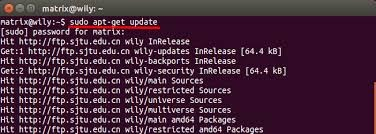
\includegraphics[width=1\textwidth]{../figures/1aptupdate.jpg} 
\caption{sudo apt-get update}
\label{update}
\end{center}
\end{figure}
Pada Gambar \ref{update} menjelaskan tentang untuk memperbaharui daftar paket.
\begin{figure}[h]
\begin{center}
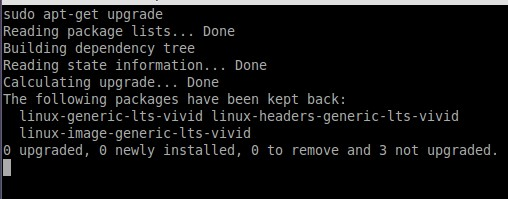
\includegraphics[width=1\textwidth]{../figures/1aptupgrade.jpg} 
\caption{sudo apt-get upgrade}
\label{upgrade}
\end{center}
\end{figure}

Pada Gambar \ref{upgrade} menjelaskan tentang untuk memperbaharui perangkat lunak sistem.
\item Proses Instalasi PIP di linux \\
Proses instalasi PIP di linux sangat sederhana karena hanya melakukan command satu perintah di Terminal.\\
\begin{figure}[h]
\begin{center}
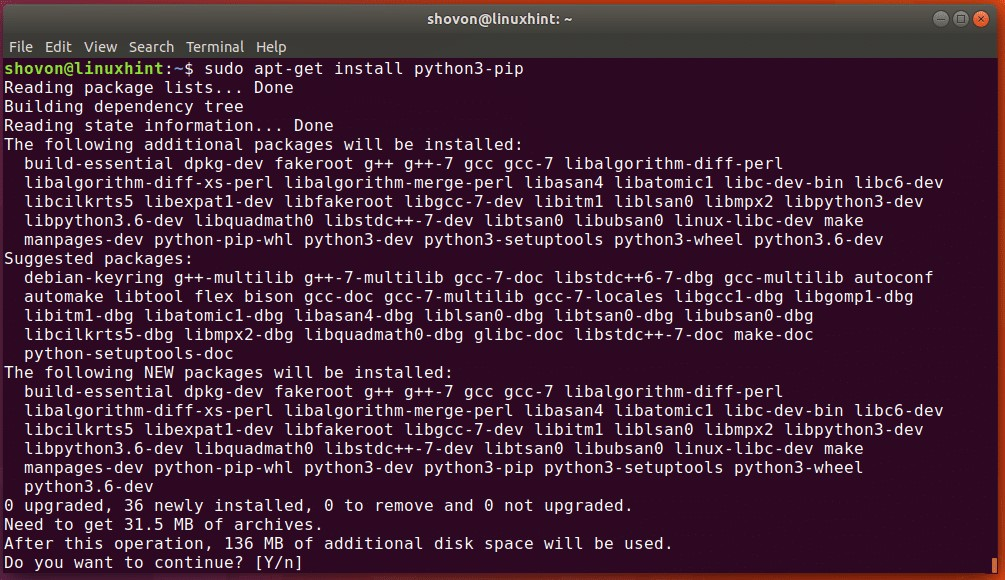
\includegraphics[width=1\textwidth]{../figures/1aptinstal.jpg} 
\caption{sudo apt-get update}
\label{instal}
\end{center}
\end{figure}
Pada Gambar \ref{instal} menjelaskan tentang proses melakukan instalasi pyhton.
\item Verifikasi PIP \\
Proses ini untuk menverifikasi apakah pip dan semua dependensi sudah terinstal atau belum agar dapat berjalan dengan optimal.\\
\begin{figure}[h]
\begin{center}
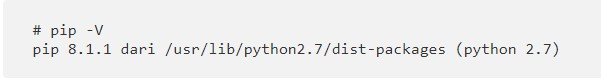
\includegraphics[width=1\textwidth]{../figures/1aptver.jpg} 
\caption{Pip -V}
\label{versi}
\end{center}
\end{figure}

Pada Gambar \ref{versi} menjelaskan tentang untuk menunjukkan versi pip yang telah diinstal.
\subsection{Instalasi PIP di Linux}
Pada umumnya perangkat python merupakan perangkat lunak yang termasuk di dalam disribusi Linux. Untuk linux distribusi slackware digunakan Python versi 2.4, yang terdapat pada CD I direktori/slackware/d. Menggunakan Toolkit untuk melakukan installasi paket di slackware adalah installpkg, berikut langkah instalasinya.\\
\item  mount/mnt/cdrom\\
\item  cd/mnt/cdrom/slackware/d\\
\item  installpkg python-2.4.1-i486-1tgz\\
\\
Python adalah menyediakan modus interaktif yang sangat berguna dalam melakukan latihan dan tes kode. Untuk menulis kode dalam modus interaktif dilakukan dengan memanggil toolkit python pada shell Linux. \\
\item  python\\
\item Python 2.4.1 (1, Apr 10 2005, 22:30:36) \\
\item GCC 3.3.5 on linux2 \\
\item Type "help", "copyright", "credits" or "license" \\
\item for more information.\\
\item  >>>\\
 Tanda “>>>” merupakan suatu prompt dalam modus interaktif Python, selanjutnya Python siap menerima input kode yang dimasukkan.\\

\section{Perintah Dasar PIP}
\subsection{Perintah Bantuan dalam PIP}
Berikut beberapa fungsi yang dapat membantu pengguna ketika dalam menggunakan PIP, antara lain :
\subsubsection{Help}
\begin{figure}[h]
\begin{center}
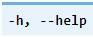
\includegraphics[width=1\textwidth]{../figures/1help.jpg}
\caption{Fungsi Help}
\label{FungsiHelp}
\end{center}
\end{figure}
Pada Gambar \ref{FungsiHelp} menjelaskan bahwa salah satu fungsi dalam PIP yang dapat menunjukkan bantuan.
\subsubsection{Version}
\begin{figure}[h]
\begin{center}
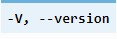
\includegraphics[width=1\textwidth]{../figures/1versi.jpg} 
\caption{Fungsi Version}
\label{fungsiversi}
\end{center}
\end{figure}
Pada Gambar \ref{fungsiversi} menjelaskan tentang salah satu fungsi pada PIP yang dapat menunjukkan versi PIP yang kita gunakan.
\subsubsection{Cache}
\begin{figure}[h]
\begin{center}
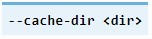
\includegraphics[width=1\textwidth]{../figures/1cache.jpg} 
\caption{Fungsi cache}
\label{fungsicache}
\end{center}
\end{figure}
Pada Gambar \ref{fungsicache} menjelaskan tentang salah satu fungsi pada PIP yang dapat mmenyimpan data cache ke direktori %<dir>
\subsubsection{No Cache}
\begin{figure}[h]
\begin{center}
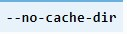
\includegraphics[width=1\textwidth]{../figures/1nocache.jpg} 
\caption{Fungsi NoCache}
\label{fungsinocache}
\end{center}
\end{figure}
Pada Gambar \ref{fungsinocache} menjelaskan tentang salah satu fungsi pada PIP untuk menonaktifkan cache
\subsection{Dasar PIP}
Ada beberapa aturan dalam menangani penggunaan string python yang dapat diandalkan :
\item Tanda kutip tunggal (') atau tanda kuutip ganda (")
\item Apabila dalam penggunaan suatu string terdapat karakter kutip tunggal (') penulisannya diapit kutip ganda (")
\item Apabila dalam penggunaan suatu string terdapat karakter kutip tunggal (") penulisannya diapit kutip ganda (')
\subsection{Perintah Dasar PIP}
Ada beberapa sintaks dasar dalam pemrograman python.
1.	Insialisasi variable. Inisialisasi variable atau statement penugasan adalah sintaks dasar dalam python, contohnya a = 2. Angka 2 adalah identitas dari variable a. Selain itu, ada juga yang dinamakan statement multi baris yang ditandai dengan beberapa baris yang terdapat symbol slash (/"). Ada pula yang dinamakan statement tanda kurung '[]','{}','()" tanpa ada slash (/")
2.	Baris dan indentasi. Kode blok yang digunakan di python menggunakan spasi (indentasi). Jumlah spasi setiap baris yang ada dalam satu blok harus sama dan sesuai.
3.	Tanda kutip dalam python. Python menggunakan tanda kutip ('), (""), ('"), ("") untuk menandai string.
4.	Komentar di python. Tidak seperti Bahasa pemrograman lain yang umumnya menandai komentar denga symbol backslash (\"). Di pemrograman python, komentar di tanadi denga symbol tetagar (\#).
\subsection{Perintah Dasar PIP}
Perintah-perintah dasar pip
Disini saya akan menjelaskan tentang instalasi package
1.	Untuk perintah instalasi package menggunakan perintah $pip install <nama-package>
2.	Bisa menambahkan versi sesuai yang diinginkan dibelakangnya contohnya $pip install <nama-package>=2.0.1
3.	Sebagai contohnya, disini akan menginstal pafy dengan menggunakan perintah $ pip install pafy
4.	Lalu uji dengan perintah $python -c import pafy
5.	Dan selesai..

\section{Contoh Penggunaan PIP}
\subsection{Contoh penggunaan PIP} 
Contoh Pengguaan pip dalam Proses enkripsi dan deskripsi suatu file dengan algoritma Huffman di implementasikan dalam bahasa python.
\item	Fungsi main
Digunakan perintah python [compress/decompress] [filename] untuk argumen “compress” untuk mengenkripsi dan memampatkan file dan argumen decompress untuk membuka kembali menjadi file.
\item	Fungsi ENCODE
Hasil file yang di enkripsi adalah Namafile+’Compressed.txt’.
\item	Fungsi DECODE
Hasil file adalah NamaFile + ’decompressed.txt’.
\subsection{Contoh penggunaan PIP}
Kita dapat melakukan install package-package yang dibundel dengan file berekstensi whl melalui PIP,wheel adalah format arsip yang digunakan untuk mempercepat melakukan penginstalan package. Setelah melakukan penginstalan wheel, lakukan penginstalan paket dengan menggunakan perintah pip install nipype-0.10.0-py2-none-any.whl . Untuk menampilkan package-package yang telah di install gunakan perintah pip list dan untuk menguninstall package lakukan dengan perintah pip uninstall <nama-package>.
\subsection{Instalasi Package Sekaligus}
Pada PIP, kita dapat melakukan penginstalan package sekaligus lebih dari satu package dan  kita tdiak perlu repot untuk menginstal satu per satu package. Pada PIP, untuk menginstal package sekaligus menggunakan requirement.txt, dimana kita melakukan list package yang akan di list dan dimasukkan dalam requirement.txt tersebut. Lalu kita ketikkan perintah
\begin{figure}[h]
\begin{center}
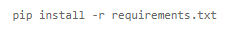
\includegraphics[width=1\textwidth]{../figures/1requre.png}
\caption{Perintah Instal Package Sekaligus}
\label{1require} 
\end{center}
\end{figure}
Pada gambar \ref{1require} menjelaskan tentang bagaimana cara instal package sekaligus dalam satu waktu.
\end{itemize}
\subsection{Contoh Penggunaan PIP}
Contoh penggunaan PIP;
PIP atau biasa dikenal dengan Python Index Packaging dapat dijalankan di berbagai Operating System, di antaranya : System Linux/Unix, Windows, Mac OS X, Java Virtual Machine, OS/2, Amiga, Palm, dan Symbian. Dalam penggunaannya, PIP sangat cocok untuk developing aplikasi berbasis WEB, Developing aplikasi berbasis GUI, Game Developing baik di computer atau mobile, dan masih banyak lagi.
\subsection{Contoh Penggunaan PIP}
Contoh penggunaan PIP;\\
A. Instalasi kebutuhan server
Tahap ini membutuhkan library python dan beberapa modul library python yang diperlukan untuk mempermudah proses development program.\\
1.Update repository\\
Dilakukan update dengan cara apt-get update\\
2. instalasi library python\\
apt-get install python-dev python-setuptools python-pip mongodb gcc\\
3. instalasi library python\\
pip install –r requirements.txt
\subsection{Contoh Pemanfaatan PIP}
Pemanfaatan Raspberry Pi untuk Hacking dan Forensic dengan metode NIST (National Institute of Standards and Technology)
Cybercrime dilakukan oleh orang yang tidak bertanggung jawab dengan tujuan merusak, memodifikasi dan menghilangkan data seseorang, salah satunya dengan menggunakan teknik hacking untuk masuk kedalam sebuah penyimpanan data untuk melakukan kejahatan.  Maka penelitian yang dilakukan adalah melakukan analisis terhadap bukti digital pada jaringan berbentuk pcap dan bukti elektronik berupa flashdisck sebagai media penyimpanan, dengan memanfaatkan Raspberry pi dan NIST.
\subsection{Contoh Pemanfaatan PIP}
Salah satu manfaat Rasberry Pi adalah bisa digunakan sebagai Mini PC untuk controlling dan monitoring suatu perangkat. Salah satu fungsi Raspberry Pi, yakni web server memanfaatkan fitur GPIO (General Purpose Input Output) pada Raspberry Pi. Berkat pemanfaatan ini, setiap perangkat elektronik di rumah dapat di control. Untuk mengontrolnya, menggunakan komunikasi pengontrolan web server melalui protocol TCP/IP serta HTTP.
\end{document}

%\chapter[Penggunaan Aplikasi Testing WebService]
%{Common Gateway Interface}
%\documentclass[12pt,a4paper]{article}
\usepackage[left=3.00cm, right=2.00cm, bottom=2.00cm, top=3.00cm]{geometry}
\begin{document}
\title{Pemanggilan Modul}
\maketitle
\begin{enumerate}
\item Fransiscus Ivan Martongam      1164039 \\
\item Lalita Chandiany Adiputri      1164043\\
\item Eko Cahyono Putro              1164035\\
\item Lidwina Triniska Gulo          1164044\\
\item Sulpadianti Bunyamin           1164096\\
\end{enumerate}


\section{Pengenalan WebService}
Web Services dengan arsitektur REST digunakan oleh berbagai macam jenis client seperti mobile, Web, dan Desktop.
Dapat membantu perusahaan untuk melakukan pelacakan, tracking terhadap tenaga penjual yang ditugaskan untuk menawarkan 
barang atau penagihan ke pelanggan. Dengan REST Web Services yang akan dibuat perusahaan akan dapat memastikan
bahwa semua tenaga penjual akan mengunjungi pelanggan sesuai dengan target yang sudah ditentukan oleh perusahaan.


\section{Arsitektur Web Services}
Architektur Web Service memiliki tiga komponen utama diantaranya yaitu Service provider adalah Penyedia web service yang berfungsi
menyediakan kumpulan web services yang dapat diaksesoleh pengguna.Service requesto adalah aplikasi yang bertindak sebagai pengguna yang
melakukan permintaan layanan (berupaweb services) keservice provider.Service registry adalah tempat dimana service provider 
mempublikasikan layanannya. Pada arsitekturWeb service,Service registry bersifat opsional.


\section{rest dalam penggunaan testing web service}
REST adalah filosofi desain yang mendorong untuk menggunakan protokol dan fitur yang sudah ada pada Web. Pada web services akan dapat memaksimalkan kinerja web services terutama pada performa, skalabilitas, dan kemudahan untuk dimodifikasi. Bentuk web service menggunakan REST style digunakan sebagai backend dari aplikasi berbasis mobile karena cara aksesnya  mudah dan hasil data yang dikirimkan berformat JSON sehingga ukuran file menjadi lebih kecil. 


\section{web api}
Web API adalah antar muka program dari sistem yang dapat diakses lewat method dan
header pada protokol HTTP yang standar. Web API dapat diakses dari berbagai macam HTTP
client seperti browser dan perangkat mobile. Web API juga memiliki keuntungan karena
menggunakan infrastruktur yang juga digunakan oleh web terutama untuk penggunaan caching
dan concurrency.


\section{Perancangan Sistem}
Aplikasi yang akan dibuat terdiri dari dua bagian besar yaitu aplikasi yang ada pada bagian client dan bagian server. 
Aplikasi yang ada di server bertugas menyediakan data yang dapat digunakan oleh aplikasi client, aplikasi client digunakan
untuk meminta data dari aplikasi yang ada di server.Web services dipilih dengan beberapa pertimbangan yaitu agar 
memudahkanpembangunan proses bisnis yang dapat digunakan untuk berbagai macam client tanpa harus membuat proses 
tersebut secara spesifik berdasarkan teknologi client yang digunakan.


\section{Implementasi Web service Berbasis ASP.NET}
Dalam proses pembuatan Web Services berbasis ASP.NET terdapat beberapa services atau fungsi-fungsi
yang dibuat untuk mengakses database SQL Server. Services-services tersebut yang nantinya dipanggil 
dan digunakan untuk membangun sistem integrasi layanan puskesmasdan rumah sakit berbasis Web Services.
Proses integrasi sistem dengan Web Services berbasis asp dapat dilakukan dengan penggunaan dokumen WSDL
yang dapat diakses pada alamat WSDL-nya http://192.168.1.100:8080/wsrs/Service.asmx?WSDL dan hasil dari skema WSDLnya.


\section{Implementasi Web service Berbasis PHP}
Pembuatan Web Services berbasis PHP dan database MySQL, terdapat  services atau fungsi yang sama 
dengan Web Services yang dibuat dengan ASP.NET. Sevices tersebut akan dipanggil dan digunakan untuk 
integrasi kedalam system berbasis Web Services. Beberapa fungsi yang terbentuk adalah sama dengan fungsi 
yang terbentuk pada hasil pembuatan Web Services berbasis ASP NET.


\section{Hasil Integrasi Web Services}
Sistem integrasi  layanan yang terdapat pada rumah sakit yang dimaksudkan menggunakan teknologi Web Services 
yang berbeda dan database yang berbeda pula. Rumah sakit AMC menggunakan database MySQL, dan PHP sebagai Web Servicesnya.
Kemudian untuk Rumah sakit umum menggunakan SQL Server sebagai databasenya, dan ASP.NET sebagai tool untuk membuat Web Servicesnya.


\section{Hasil Sistem integrasi  layanan puskesmas dan rumah sakit}
Layanan informasi merupakan halaman awal yang ditampilkan ketika client tersebut diakses menggunakan web browser. 
Setelah Itu pengguna melakukan pemilihan kriteria kelengkapan rumah sakit, pengguna harus mengisi data-data pasien yang mendaftar pada rumah sakit. Selanjutnya user  menampilkan data dokter, data kamar, data fasilitas, data pasien, dan juga data registrasi pasien pada rumah sakit.


\section{Analisis Hasil Pengujian dan Implementasi}
Aplikasi berjalan sesuai dengan analisis masalah dan kebutuhan sistem.
Pengujian sistem yang pertama dilakukan adalah testing pada web service itu sendiri 
dan dilanjutkan dengan testing pada fungsi-fungsi  yang terdapat pada masing-masing web service. 
selanjutnya dilakukan testing aplikasi web service melalui aplikasi web interface yang menggunakan bahasa pemrograman ASP.NET dan PHP.
Web Service yang berfungsi sebagai Middleware serta melakukan pertukaran data dalam format XML melalui sebuah jaringan dengan menggunakan protokol standar internet.


\section {Google Map Service}
Google Map Service adalah sebuah jasa peta global virtual gratis dan online yang
disediakan oleh perusahaan Google. Google Maps dapat ditemukan di alamat
http://maps.google.com.Google Maps menawarkan peta yang dapat diseret dan gambar
satelit untuk seluruh dunia.Google Maps juga menawarkan pencarian suatu tempat dan
rute perjalanan.
\subsection {Google Maps API }
Google Maps API adalah sebuah layanan (service) yang diberikan oleh Google
kepada para pengguna untuk memanfaatkan Google Map dalam mengembangkan
aplikasi. Google Maps API menyediakan beberapa fitur untuk memanipulasi peta, dan
menambah konten melalui berbagai jenis services yang dimiliki, serta mengijinkan
kepada pengguna untuk membangun aplikasi enterprise di dalam websitenya.


\section{Global Positioning System (GPS)}
Global Positioning System, adalah sistem atau sarana yang digunakan untuk memberikan informasi dimana keberadaan pengguna secara umum dipermukaan bumi yang berbasiskan satelit. Data dikirim dengan data digital. GPS dapat digunakan dimanapun juga dalam 24 jam. Posisi unit GPS akan ditentukan berdasarkan titik-titik koordinat latitude dan longitude, maka GPS bisa membantu menunjukan arah. 


\section{Geolocation}
Geolocation adalah sebuah cara untuk mengetahui suatu lokasi di dunia. Ada beberapa metode untuk menemukan lokasi, yaitu dengan IP address, sambungan wireless atau BTS, dan dedicated GPS atau embeded GPS pada telepon seluler. Geolocation selain menggunakan data koordinat latitude, selain itu geolocation juga menggunakan longitude yang dimiliki oleh komputer atau telepon seluler.


\section{Framework CodeIgniter}
CodeIgniter merupakan salah satu dari sekian banyak framework PHP yang  bertujuan dari pembuatan framework CodeIgniter ini adalah untuk menghasilkan framework  yang dapat digunakan untuk pembuatan proyek website secara lebih cepat dibandingkan dengan pembuatan website secara manual.
Salah satu keuntungan menggunakan framework codeigniter adalah, gratis, berjalan di php versi 4 dan 5, ringan dan cepat, mempunyai fitur-fitur yang lengkap dan menggunakan metode MVC (Model View Controller).



\section{Project Management and requirement}
Data warehouse yang dikembangkan adalah data warehouse yang dioptimasi untuk kepentingan evaluasi akademik Fakultas Teknologi Informasi. Fungsi evaluasi mencakup nilai mahasiswa, absensi dan hasil studi yang dapat dianalisa berdasarkan program studi, tahun ajaran, lokasi kuliah, dan angkatan mahasiswa. Berdasarkan pengumpulan data yang dilakukan, dilakukan analisa kebutuhan yaitu: Model data warehouse yang mampu digunakan oleh EIS, Dibutuhkan sebuah metode distribusi yang bersifat independen, sumber data yang mampu menampilkan laporan dan analisa


\section{Permodelan Data Warehouse Dimensional}
Sebagai sumber data untuk data warehouse, digunakan sumber data operasional yang menyimpan data harian dari sistem akademik. Database harian yang digunakan  oracle DBMS 6 yang menyimpan data–data akademik yaitu: mahasiswa, rencana studi, nilai, absensi, mata kuliah, jadwal, kurikulum, pembimbing akademik, dan lainnya. Untuk model skema yang digunakan star schema, dimana satu tabel fakta dikelilingi oleh beberapa tabel dimensi. 


\section{Pengembangan Model Distribusi Web Service}
Model distribusi data warehouse yang akan dikembangkan berbasis web service dengan framework WSF/PHP.    
Web service pada penelitian ini dapat diakses menggunakan SOAP (Simple Object Access Protocol) dengan transport layer http. 
Tiap client yang mengakses harus membuat instance dari kelas WSClient dan mengirim XML format request. 
Untuk dapat digunakan aplikasi desktop, sebuah consumer bertindak sebagai intermediate untuk mengembalikan format XML.


\section{Aspek manajerial}
Dari sisi manajerial, pemanfaatan data warehouse dengan distribusi web service
memberikan beberapa perubahan pada proses bisnis analisa data. Pihak manajemen
dapat langsung menganalisa informasi yang disediakan data warehouse, memberikan
peningkatan kualitas informasi yan dijadikan basis pengambilan keputusan. Pihak manajemen juga dapat mengurangi
campur tangan pengembang EIS dari akses skema data yang tidak berhak. Tanggungjawab pengembangan dan web service
menjadi terpisah dari EIS. 


\section{Aspek sistem}
Dari sisi sistem, keuntungan utama ialah adanya data warehouse yang terpisah dari data operasional, sehingga meningkatkan kesederhanaan proses retrieve data dan peningkatan kinerja sistem. Skalabilitas dari sistem menjadi lebih baik, karena jika ada perubahan teknologi atau perubahan struktur pada sisi data warehouse, tidak akan mempengaruhi aplikasi pengguna (tidak perlu dilakukan perubahan). 
Penggunaan web service sebagai intermediate antara data warehouse dan aplikasi pengguna meningkatkan modularitas dan fleksibilitas dari data yang disajikan.


\section{Aplikasi SIG Terintegrasi yang Dikembangkan Menggunakan “Big” Web Service}
Pengembang aplikasi SIG akan menggunakan/memanfaatkan layanan (service) “Big” Web Service, karena “Big” Web Service memiliki standar
pesan SOAP (Simple Object Access Protocol), maka data berformat GML yang ada di basis data XML
terlebih dahulu harus diubah dulu ke format SOAP yang memiliki elemen XML peringkat teratas
 (envelope) dan yang memuat di dalamnya elemenelemenheader dan body.Program Java yang pengembang aplikasi SIG buat harus mampu
menyusun/merakit pesan SOAP yang berisi data berformat GML, dimana dalam hal ini XML Schema bisa digunakan untuk mendeskripsikan struktur internal pesan SOAP itu. Untuk melakukan hal ini, pada aras rendah pengembang aplikasi SIG bisa
melakukannya dengan membuat suatu lapisan program kecil (adapter) yang memanfaatkan API
SAAJ (Simple Object Access Protocol with Attachments API for Java), yang memiliki antarmuka DOM
(Document Object Model) Node, yang merupakan kelas dasar dari semua kelas dan antarmuka
(interface) yang ada di dalam pesan-pesan SOAP.
\subsection{Aplikasi SIG yang terintegrasi menggunakan "Big"Web Service}
Menggunakan API SAAJ, seperti sesuai dengan peringkatnya yaitu berada di aras rendah, kita bisa merakit pesan SOAP dari data GML yang berasal dari sistem basis data XML yang kita gunakan. Alternatif lainnya, kita bisa menggunakan XSLT (eXtensible Stylesheet Language Transformation), yang merupakan suatu API dalam bahasa pemrograman Java yang dapat melakukan transformasi dokumen GML menjadi dokumen SOAP, asalkan kita menyediakan/memliki XSLT-Stylesheet-nya.


\section{Aplikasi SIG Terintegrasi yang Dikembangkan Menggunakan RESTful Web Service}
REST (REpresentational State Transfer) sejak awal memang memang diperkenalkan sebagai arsitektur sistem untuk mengembangkan sistem/aplikasi hypermedia yang berskala besar, yang digunakan terutama berbasis pada protokol HTTP. erutama berbasis pada protokol HTTP. Arsitektur REST (POX-HTTP/Plain Old XML over HTTP) bersifat Identifikasi sumberdaya menggunakan URL
(Uniform Resource Locator), Antarmuka yang seragam, yaitu PUT, GET,POST, dan DELETE, Pesan-pesan yang bersifat deskriptif, Interaksi di dalam aplikasi SIG dilakukan melalui hyperlink.
\subsection{Aplikasi SIG Terintegrasi yang Dikembangkan Menggunakan RESTful Web Service}
Saat kita melakukan integrasi aplikasi SIG atas berbagai sistem basisdata XML menggunakan RESTful Web Service, kita bisa langsung melakukan pemetaan operasi CRUD XQuery untuk sistem basisdata XML itu ke operasi CRUD yang berpadanan pada RESTful Web Service 
untuk melakukan integrasi atas data GML yang berasal dari beberapa sistem basis data XML bisa dilakukan dengan menggunakan URL untuk setiap sistem basis data XML itu, kemudian aplikasi SIG bisa menvisualisasikannya ke dalam bentuk aplikasi SIG terintegrasi


\section{Perbandingan Antara “BIG” Web Service dengan RESTFul Web Service untuk Integrasi Data Berformat GML}
Implementasi Java Web Service menggunakan “Big” Web Service dengan implementasinya menggunakan RESTful Web Service [1, 2, 3, 4, 6, 8, 9, 14, 16, 19] saat pengembang aplikasi bekerja untuk suatu aplikasi SIG terintegrasi. Perbedaan karakteristik akan menimbulkan implikasi yang berkaitan dengan kelebihan serta kelemahannya masing masing. Karena hal-hal itu sangat bergantung pada preferensi pengembang aplikasi SIG serta sangat bergantung pada sumberdaya manusia (analis sistem dan pemrogram) yang diperlukan untuk mengembangkan aplikasi SIG terintegrasi yang memanfaatkan sistem basis data XML.

\end{document}

\chapter[Pemanggilan Modul]
{Common Gateway Interface}


\section{Modularitas dan Portabilitas}
Modularitas dan portabilitas merupakan faktor pentig karena termasuk atribut kualitas perangkat lunak. Modularitas berasal dari kata modul, modul adalah bagian perangkat lunak yang besar yang dipecah menjadi bagian yang lebih kecil dengan memberi nama. Pengalamatan memori berbeda beda kemudian diintergrasikan untuk membentuk perangkat lunak yang dapat memenuhi kebutuhan dari suatu permasalahan

\section{Paradigma Berorientasi Obyek}
Paradigma berorientasi obyek adalah suatu cara mengorganisasikan perangkat lunak sebagai kumpulan obyek- obyek yang memiliki sifat (struktur data) dan perilaku (fungsi) yang saling berinteraksi melalui pesan (message). Konsep yang menjadi pilar paradigma berorientasi obyek adalah : abstraction, encapsulation, inheritance, polymorphism. Abstraksi dipresentasikan sebagai suatu kelas yang digunakan untuk instansiasi objek.

\subsection{Obyek dan Class}
Obyek (object) merupakan representasi dari entitas sebagai sarana pembungkusan karakteristik struktural
yang dapat disebut atribut dan karakteristik perilaku yang disebut operasi (operation/method). Atribut 
mempresentasikan karakteristik entitas yang menentukan keadaan suatu obyek jika menerima pesan.
Operasi tersebut dapat berupa prosedur maupun fungsi. Kelas merupakan deskripsi dari suatu obyek pada 
saat implementasi (coding).


\subsection{Penurunan Sifat}
Penurunan sifat (inheriatance) adalah kemampuan suatu obyek mewarisi sifat dari obyek yang lain. Kemampuan ini menghasilkan program yang efesien karena ada mekanisme pemakaian kembali (resauble) kode program. Pemograman yang dibuat dapat menggunakan fungsi yang ada dalam file DLL dengan mengirim parameter dan menerima balikan dari fungsi dan selama dapat mengikuti kesepakatan dalam pemangglan fungsi atau prosedure tersebut.


\section{Dynamic link library}
System operasi windows dapat menggunakan proses linker konvensional (proses linker secara statis) dengan file berinteraksi LIB dan dapat secara dinamis menggunakan dynamic link library (DLL).
proses linking fungsi dari DLL secara fisik tidak disalin dan digabung kedalam executable file tetapi tetap terpisah dan dipanggil oleh executable file (“client”) pada saat runtime.

\section{Perancangan Modul-modul Pengembangan}
\subsubsection{Perancangan Modul Pengiriman SMS}
Mekanisme pengiriman SMS yang digunakan adalah pengiriman melalui telepon selular. Telepon selular yang digunakan tersebut dihubungkan ke Komputer menggunakan kabel data. Ketika sinyal datang, program yang berada pada Komputer akan menginstruksikan telepon selular untuk mengirimkan pesan ke nomor telepon selular pemilik rumah.
mengenali instruksi ini sebagai instruksi AT Command untuk mengirim SMS. AT command merupakan instruksi-instruksi yang digunakan untuk mengendalikan telepon seluler atau modem GSM/GPRS yang dihubungkan ke Komputer.
\subsection{Perancangan Modul Dial-Up}
Modul dial merupakan modul didalam sebuah software isi ulang pulsa dengan metode dial atau call.Jika menggunakan handphone kita sering menggunakan metode dial ini ketika cek pulsa. Biasanya modul dial diawali dengan karakter bertanda bintang (*) 
dan diakhiri karakter tagar. Modul dial up membutuhkan modul mikrokontroler tambahan 
sebagai antarmuka antara mikrokontroler dan kabel telepon. Modul ini hanya dapat dihubungkan dengan 
sebuah mikrokontroler DT-51 MinSys.
\subsection{Dataset Modul Deteksi Plagiarisme}
Data yang digunakan pada modul ini berupa kode program mahasiswa dalam satu kelas. Kode program tersebut merupakan hasil pengerjaan tugas pemrograman yang diberikan oleh dosen Teknik Informatika ITS. Data yang diambil terdiri dari dua jenis kode program mahasiswa dalam satu kelas yang mengambil mata kuliah Pemrograman Berorientasi Objek (PBO). Dataset jenis pertama berjumlah 38 buah kode program dari 38 mahasiswa dalam satu kelas. Dataset jenis ke 2 berjumlah 21 buah kode program dari 21 mahasiswa dalam satu kelas. Pada dataset jenis kedua terdapat dua jenis file yaitu 21 file header (.h) dan 21 file yang berekstensi .cpp. Sehingga masing-masing file akan dihitung perfomanya pada tahap uji coba.
\subsection{Dataset Modul Student Feedback System}
Data-data yang digunakan pada modul ini berasal dari tugas mata kuliah Pemrograman Berorientasi Objek (PBO) Kelas C Tahun Ajaran 2013/2014 di Jurusan Teknik Informatika ITS. Dataset yang digunakan adalah tiga jenis dataset, yaitu dataset class Invoice, class Account, serta dataset kode sumber yang tidak mirip. Jumlah dataset pertama yaitu 31 buah kode program mahasiswa, jumlah dataset kedua adalah 31 buah mahasiswa, dan jumlah dataset ketiga adalah 9 mahasiswa.


\section{Pembuatan Modul-modul Pengembangan}
\subsection{Pembuatan Modul Pengiriman SMS}
Pengiriman SMS dilakukan dengan cara menghubungkan telepon selular ke PC menggunakan kabel data. 
Program yang digunakan untuk mengirimkan SMS menggunakan bahasa pemrograman Microsoft Visual Basic.NET 2003. Program ini membutuhkan library tambahan yang berisi class-class yang dapat digunakan untuk komunikasi ke telepon selular. Library yang digunakan adalah GSMComm yang dapat diunduh secara gratis dari internet. 
\subsection{Pembuatan Modul Dial-Up}
Mekanisme dial up dilakukan dengan menambahkan sebuah modul mikrokontroler ke dalam rangkaian mikrokontroler yang ada
Modul tambahan ini berfungsi sebagai antarmuka mikrokontroler ke kabel telepon atau ke pesawat telepon. Modul ini kompatibel penuh dengan mikrokontroler. 
Program untuk mengoperasikan rangkaian mikrokontroler ini dibangun dengan menggunakan bahasa assembler untuk mikrokontroler yang selanjutnya dikompilasi menjadi format Hexadesimal.


\section{Implementasi Modul}
\subsection{Implementasi Modul Pengiriman SMS}
Program yang dibuat berdasarkan algoritma pengiriman SMS dienkapsulasi menjadi sebuah modul. Penyisipan fungsi pemanggilan modul pengiriman SMS dilakukan sebelum program tersebut mengirimkan sinyal ke komputer server melalui jaringan nirkabel IEEE 802.11. Dengan demikian, diharapkan agar SMS diterima oleh pemilik rumah tidak lama setelah petugas keamanan mendapatkan sinyal. 
\subsection{Implementasi Modul Dial Up}
Modul dial up yang dibuat dengan bahasa assembler dienkapsulasi menjadi sebuah fungsi yang dapat digunakan dan dipanggil oleh program assembler lain. Pemanggilan fungsi dial up ini dilakukan setelah prosedur pengiriman data ke komputer melalui komunikasi serial.
\subsection{Menerima Pesan dalam Bentuk PDU}
Menerima pesan dalam bentuk PDU tidak hanya isi pesan saja, melainkan terdapat berbagai data di dalamnya seperti informasi mengenai pengirimnya (nomor telepon pengirim), SMSC, dan Waktu Pengiriman Pesan. Data yang masuk berupaHexa – Decimal Octets. SMSC yaitu menerangkan banyaknya informasi pengirim yang terdapat pada pesan yang digunakan oleh pengirim.
\subsection{Mengirim Pesan dalam Format PDU}
Pesan ditulis dalam format text akan di konversikan terlebih dahulu kedalam format PDU agar bisa di baca oleh HP. PDU, adalah proses yang akan memanggil modul konversi untuk merubah data dalam Format Text menjadi Format PDU.  Alur proses kirm SMS, masukan berupa Format Teks dikonversi ke bentuk Format PDU.
\subsection{Modul Form Pendaftaran Antrian}
Digunakan oleh konsumen untuk pendaftaran antrian. Berisi nomor antrian sebelumnya, waktu tunggu, pilihan untuk memilih jenis pelanggan (telpon/Flexi atau Speedy atau calon pelanggan), field untuk memasukkan nomor telpon/Flexi/selular, link menuju form Pendaftaran. Antrian 2 bagi calon pelanggan, pilihan jenis layanan berupa checkbox, tombol Daftar Antrian, tombol Batal.
\subsection{Modul Form Login Petugas}
Form login petugas digunakan untuk masuk ke dalam aplikasi untuk supervisor. Form login petugas ini berisi
field untuk mengisi username, password, dan nomor meja tempat bertugas. 
\subsection{Modul Form Input Pelayanan Konsumen}
Modul ini akan muncul setelah tombol Panggil Antrian Berikutnya dan tombol Panggil pada form CallNextCus ditekan. 
Dalam modul ini berisi data identitas konsumen, pilihan untuk masukan jenis produk berupa drop down list,
field untuk memasukkan data masalah dan solusi, tabel berisi data sejarah konsultasi konsumen sebelumnya, tombol Simpan, tombol
Batal, dan tombol Ubah Data Konsumen. 
\subsection{modul From Ubah Data Konsumen}
Modul ini akan muncul setelah tombol Ubah Data Konsumen ditekan. Dalam modul ini berisi data identitas konsumen yang ada dalam field-field dan bisa mengubahubah isinya, tombol Simpan akan mengubah jika ditekan menuju form Input Pelayanan Konsumen, tombol Batal, dan tombol Keluar akan mengubah jika ditekan menuju form Input Pelayanan Konsumen.
\subsection{Modul Form Display}
Modul form display ini berisi nomor antrian yang dipanggil, nomor meja petugas yang memanggil, dan daftar meja beserta petugas yang bertugas (jika petugas login maka namanya akan muncul dan jika logout namanya akan hilang. Nomor antrian dan nomor meja berubah setiap kali petugas menekan tombol Panggil Antrian Berikutnya pada form CallNextCus.
\subsection{Modul Form Data Konsumen}
Setelah proses login berhasil, secara default ditampilkan modul antrian. Digunakan untuk menampilkan daftar seluruh nama konsumen yang pernah datang ke Plasa. Modul ini menampilkan tabel yang berisi data data daftar nama konsumen berupa link menuju form Data Identitas Konsumen, alamat, dan nomor teleponnya. Di sebelah bawah, ditampilkan form  Pencarian data Konsumen.
\subsection{Pengujian Modul Student Feedback System}
Pengujian dilakukan dengan menilai akurasi pada penghitungan nilai kemiripan dua buah kode program, dilakukan sebanyak tiga kali menggunakan tiga buah dataset. Perhitungan kemiripan kode program dilakukan secara manual.
Pengujian kedua adalah penampilan rekomendasi kode program yang mirip. Sistem akan menampilkan kode program secara berdampingan, kode program yang sama akan diberi tanda khusus.
\subsection{Pengujian Modul Deteksi Plagiarisme}
Pengujian dilakukan dengan menilai akurasi pada penghitungan nilai yang memiliki dua buah kode program dan akurasi pengelompokan kode program dengan menggunakan jumlah cluster hasil penghitungan standar deviasi. Pengujian dilakukan menggunakan dua buah dataset yang telah dijelaskan sebelumnya. Pengujian pada penilaian akurasi pengelompokan kode program dilakukan dengan memberi label True dan False pada masing-masing anggota cluster. 

\section{Perencanaan Modul Sistem}
\subsection{Modul Terima SMS}
Modul ini berfungsi untuk menerima data PDU yang masuk dan menampung masing-masing bagian dari data tersebut.
input-an pada prosedur ini yaitu string data PDU yang belum dipisahkan sesuai dengan nama bagiannya, sedangkan pada output-nya
berupa string PDU yang sudah dipisahkan yang terdiri dari panjang nomor SMSC, tipe alamat
SMSC, nomor SMSC, Octet pertama dari pesan SMS-Deliver. Banyaknya suatu nomor berasal dari nomor pengirim, tipe alamat dari nomor pengirim, nomor telepon pengirim pesan, protokol identifier, data coding scheme, waktu pengiriman pesan, banyaknya
pesan yang dikirim dan isi pesan sesuai dengan nama bagiannya. 
\subsection{Modul Kirim SMS}
Modul kirim sms memiliki fungsi untuk menampung data yang akan dikirimkan yaitu dalam betuk format PDU, dimana dalam prosesnya akan memanggil modul konversi untuk merubah data dalam Format Text menjadi Format PDU. Alur proses kirm SMS, yakni dari masukan berupa Format Teks dikonversi ke bentuk Format PDU. 
\subsection{ Modul Konversi}
Modul ini berfungsi untuk menerjemahkan data yang masuk dari modul terima sms  format PDU menjadi  text,  melakukan pengkonversian informasi dari srting hexa menjadi biner, biner menjadi decimal,decimal menjadi character. Modul ini juga menerjemahkan data yang masuk  dari modul kirim sms format text menjadi PDU, mengembalikan posisi data PDU dari character sampai menjadi string hexa. 
\subsection{Modul Power Suply}
Modul ini berguna untuk memberikan daya yang diperlukan untuk menjalankan modul- modul tersebut. Pada power supply tersebut terdiri dari transformator, rectifier, filter dan voltage regulator. Pada perancangan power supply ini digunakan transformator dengan tipe step down atau penurun tegangan. Transformator ini digunakan untuk menurunkan tegangan dari PLN yang sebesar 220 V menjadi besar tegangan yang diinginkan, dimana pada perancangan ini tegangan yang diinginkan 5 V DC. Modul power supply berguna untuk memberi tegangan yang dibutuhkan oleh suatu alat untuk bekerja. Pada rancangan ini digunakan hanya satu buah power supply yang terletak pada modul simulasi.
\subsection{Mikrokontroler}
Mikrokontroler memiliki kemampuan untuk menyimpan dan menjalankan suatu program yang bertujuan sebagai kontrol.
Dalam sebuah IC mikrokontroler sudah terintegrasi ROM, RAM, EPROM, serial interface dan paralel
interface, timer, interrupt controller, konverter analog ke digital (ADC). Rangkaian tersebut terdapat dalam level chip atau biasa disebut single chip microcomputer.Mikrokontroler memiliki beberapa keunggulan yaitu Kehandalan tinggi dan kemudahan integrasi dengan komponen lain ,Mikrokontroler dapat mempermudah perbaikan maupun update system karena kontrolnya tidak berupa fisik,
melainkan software yang disimpan dalam Flash ROM ataupun EEPROM yang mudah diisi ulang dan Banyak kemampuan yang ditambahkan dalam sebuah chip tunggal, misalnya Timer, Serial interface, ADC,DAC, EEPROM, RTC, ISP.
\subsection{LIGHT EMITTING DIODE (LED)}
LED adalah sebuah dioda yang bisa menghasilkan cahaya apabila diberi tegangan foward bias. Ketika LED diberi tegangan foward bias, elektron bagian negatif pada dioda akan berpasangan dengan hole dari bagian positif. 
Dalam proses penyatuan tersebut, akan terjadi pemancaran energi dalam bentuk panas dan cahaya. Pada dioda Silikon dan Germanium, sebagian besar energi yang timbul dalam bentuk panas. Bahan yang biasanya digunakan untuk LED seperti Galium Arsen Phospida (Ga-AsP) dan Galium Phospida (GaP), energi yang dipancarkan dalam bentuk energi foton atau cahaya.
\subsection{Modul Interface RS-232}
Perancangan pengantrian meja pada restoran secara wireless  menggunakan  interface serial RS-232. Interface serial RS-232 berfungsi untuk mengirimkan data-data kedalam kode biner. Standar RS-232 ini dikembangkan oleh Electronics Industry Association and the Telecommunications Industry. Modul ini berguna sebagai penghubung antara modul mikrokontroler dengan komputer. Modul jaringan  dibutuhkan agar seluruh perintah komputer dapat diubah menjadi sinyal kontrol bagi mikrokontroler. 


\section{Hasil dan Evaluasi}
\subsection{Hasil dan Evaluasi Modul Deteksi Plagiarisme}
Skenario implementasi satu adalah penghitungan akurasi sistem pendeteksi plagiarisme kode program dengan menggunakan dataset jenis pertama yaitu dataset yang memiliki tingkat kemiripan antar kode program yang relatif kecil. Implementasi dilakukan dengan menghitung akurasi pada penghitungan nilai similarity antar kode program, pengelompokan kode program berdasarkan tingkat kemiripannya, dan penentuan jumlah cluster terbaik yang akan dipilih.Terdapat 38 kode program pada dataset jenis pertama yang memiliki total 703 nilai similarity.
\subsection{Hasil pengujian dan analisis}
Pengujian modul power supply bertujuan  untuk mengetahui hasil output dari power supply yang telah dirancang apakah telah sesuai dengan yang diinginkan dan untuk pengujian tersebut dilakukan dengan dua cara. Pertama yaitu pengujian hasil output dari power supply dengan tanpa beban dengan cara mengukur langsung pada output dari power supply  dan yang kedua yaitu pengujian hasil output dari power supply dengan beban dengan cara menyambung modul power supply tersebut dengan beberapa buah resistor dengan tahanan yang berbeda.



\chapter[Instalasi PIP]
{Common Gateway Interface}
\documentclass[12pt,a4paper]{article} 
\usepackage{graphicx}
\linespread{1.5}
\begin{document}
\title{Instalasi PIP dan Contoh Penggunaan}
\maketitle

\begin{itemize}
\item
Nama Kelompok 1\\
Farid Ariyanto Saputra 1164036\\
Nurgivani Syarifatul Husna 1164050\\
Velariza Alvioletta 1164056\\
Yogi Aditya Saputra 1164060 \\
\end{itemize}

\section{Python}
\subsection{Pengertian Python}
Python merupakan salah satu Bahasa pemrograman yang bersifat open source yang tertafsir oleh typing yang dinamis dan kuat. Python juga memiliki banyak library, seperti struktur data, files, dan jaringan. Bahasa pemrograman python juga banyak digunakan untuk berbagai keperluan, contohnya komputasi ilmiah, system administrasi, dan pengembangan web. Selain itu pula, keuntungan Bahasa pemrograman python yakni memiliki alat simulasi python gratis.
\subsection{Pengertian Python}
Python adalah suatu bahasa pemrograman yang bisa dikatakan bahasa pemrograman jaman sekarang, karena usianya sangat muda namun sudah banyak digunakan oleh programmer. Phyton dapat mendukung dalam membangun aplikasi berbasis desktop, web, mobile maupun lainnya. Untuk membangun sebuah aplikasi, bahasa pemrograman ini juga bisa digunakan menggunakan framework maupun tanpa framework. Namun, apabila tidak menggunakan framework akan membutuhkan waktu yang lama dalam tahap membangun aplikasi, begitu juga sebaliknya apabila menggunakan framework pembangunan aplikasi akan menjadi lebih cepat dan terstruktur, biasanya framework yang digunakan adalah Django, dimana disana terlah tersedia komponen seperti models, templates, views, forms, dan admin interface.
\subsection{Pengertian Python}
Python merupakan sebuah bahasa dalam pemrograman yang dibuat oleh Guido Van Rossum dan populer sebagai sebuah bahasa pemrograman berbasis Web. Python dikenal sebagai sebuah bahasa yang menggabungkan kapabilitas, kemahiran, dengan sintaksis kode yang jelas. Mengambil dari pengertian wikipedia, Python merupakan sebuah bahasa pemrograman interpretatif yang bisa digunakan dalam berbagai macam program web dengan filosofi perancangan yang berfokus ada tingkat keterbacaan kode.
\subsection{Pengertian Python}
Phyton merupakan salah satu Bahasa pemrograman kelas atas serta memiliki sifat intrepeter, object oriented, serta interaktif serta dapat berjalan pada sistem operasi seperti UNIX, MAC, Windows maupun platfrom lain. Karena Python merupakan bahasa pemrograman kelas tinggi, python dapat di kombinasikan dalam penggunaan tata kalimat dengan modul-modul yang telah siap pakai serta struktur data yang lebih efisien.
\subsubsection{Perbedaan Pyhton 2 dan Pyhton 3}
Berikut adalah tabel \ref{table:perbedaan} perbedaan python 2 dan python 3, yaitu :
\begin{table}[h]
\caption{Perbedaan Pyhton 2 dan Pyhton 3}
\centering
\begin{tabular}{ccc}
\hline
 &Pyhton 2&Pyhton 3\\
\hline
versi pyhton&python --version&pyhton3 --version\\
publikasikan&2000&2008\\
Fokus&Lebih Transaparan dan inklusif &perapian pada codebase\\
&untuk pengembangan&dan menghapus duplikasi\\
Coding&print "coba"  &print ("coba")\\
&tidak harus menggunakan tanda kurung& harus menggunakan tanda kurung\\
\end{tabular}
\label{table:perbedaan}
\end{table}

\section{PIP}
\subsection{Pengertian PIP}
PIP yang memiliki kepanjangan dari Pyhton Index Packaging. PIP itu sendiri adalah sebuah app store atau biasa disebut package manager yang biasa digunakan untuk mencari, mengunduh, menginstal serta mengelola package atau modules yang biasa ditemukan di PyPI ( Pyhton Package Index ). Dimana PyPI adalah sebuah library perangkat lunak untuk Bahasa pemrograman Pyhton.
\subsection{Pengertian PIP}
PIP merupakan singkatan dari python index packaging. PIP adalah sebuah aplikasi manajemen package yang biasa digunakan untuk menginstall dan mengelola package yang telah ditulis oleh python. Untuk menemukan packagenya, kita bisa mencari di situs Python Package Index (PyPI). Ada kurang lebih 134443 package dalam python yang bisa diinstall melalui PyPI.
\subsection{Pengertian PIP}
PIP (python index packaging) merupakan Package Management System yang biasanya digunakan untuk mengunduh dan mengelola package Python. Banyak sekali package yang bisa di temukan di PyPI. 
PIP bisa langsung digunakan di Python versi 2.7.9 dan versi 3 namun apabila menggunakan versi dibawahnya harus melakukan instalasi terlebih dahulu. 
Pip juga sebuah sistem untuk memeriksa perilaku sistem terdistribusi secara otomatis terhadap harapan programmer tentang sistem. Pip mengklasifikasikan perilaku sistem valid atau tidak valid, mengelompokkan perilaku ke dalam set yang dapat dipikirkan, dan menyajikan perilaku keseluruhan dalam beberapa bentuk yang sesuai untuk menemukan atau memverifikasi kebenaran perilaku sistem.
\subsection{Pengertian PIP}
PIP merupakan singkatan dari python index packaging yang merupakan package management sistem yang sering kali di gunakan untuk mengelola package python. Packages python dipasang dengan manajer paket pip, yang termasuk dalam semua lingkungan virtual. seperti sesi prompt perintah python akan memanggil versi alat ini daripada milik virtual enviroment yang diaktifkan.

\section{Cara Instalasi PIP}
\subsection{Instalasi di Windows}
Berikut adalah cara menginstall PIP atau Python Index Packaging. \\
1.	Kunjungi web resmi https://pip.pypa.io/en/stable/installing/ untuk mendownload dan melihat cara instalasi di windows.\\
2.	Download get-pip.py dari web tersebut. \\
3.	Buka Python.exe atau buka CMD dan ketikan perintah python get-pip.py di folder yang ada file get-pip.py yang sudah di 	download tadi.\\
4.	Kemudian set PATH dalam environmental variable ke tempat pip.exe. \\
5.	Untuk mengecek instalasi pip, ketikan perintah pip id di CMD. \\
\subsection{Instalasi PIP di Mac}
Disini saya akan memberitahu cara install PIP untuk mac x, caranya adalah : \\
1.	Download python terlebih dahulu pada website resminya \\
2.	Lalu akan mendapatkan file berbentuk .pkg  dari proses download yang telah dilakukan \\
3.	Selanjutnya lakukan doubleclik file tersebut dan otomatis akan memandu untuk melakukan installasi, ikuti langkah tersebut dengan menekan next pada setiap langkah-langkahnya \\
4.	Buka terminal dan tulis “python3 –version” \\
5.	Lalu, “sudo easy install pip” \\
6.	Dan, installasi selesai. \\
\subsection{Instalasi PIP di Linux}
Pada Sistem Operasi Linux, proses instalasi Pyhton tidak bermain dengan skrip getpip.py seperti di windows dan mac. Berikut adalah tahapan instalasinya.
\begin{itemize}
\item Melakukan memperbaharui daftar paket dan perangkat lunak sistem.
\begin{figure}[h]
\begin{center}
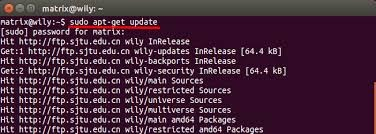
\includegraphics[width=1\textwidth]{../figures/1aptupdate.jpg} 
\caption{sudo apt-get update}
\label{update}
\end{center}
\end{figure}
Pada Gambar \ref{update} menjelaskan tentang untuk memperbaharui daftar paket.
\begin{figure}[h]
\begin{center}
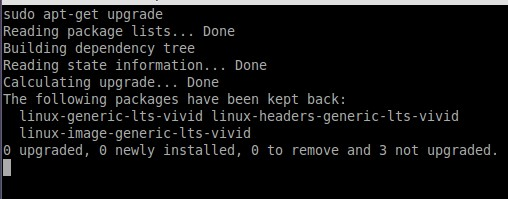
\includegraphics[width=1\textwidth]{../figures/1aptupgrade.jpg} 
\caption{sudo apt-get upgrade}
\label{upgrade}
\end{center}
\end{figure}

Pada Gambar \ref{upgrade} menjelaskan tentang untuk memperbaharui perangkat lunak sistem.
\item Proses Instalasi PIP di linux \\
Proses instalasi PIP di linux sangat sederhana karena hanya melakukan command satu perintah di Terminal.\\
\begin{figure}[h]
\begin{center}
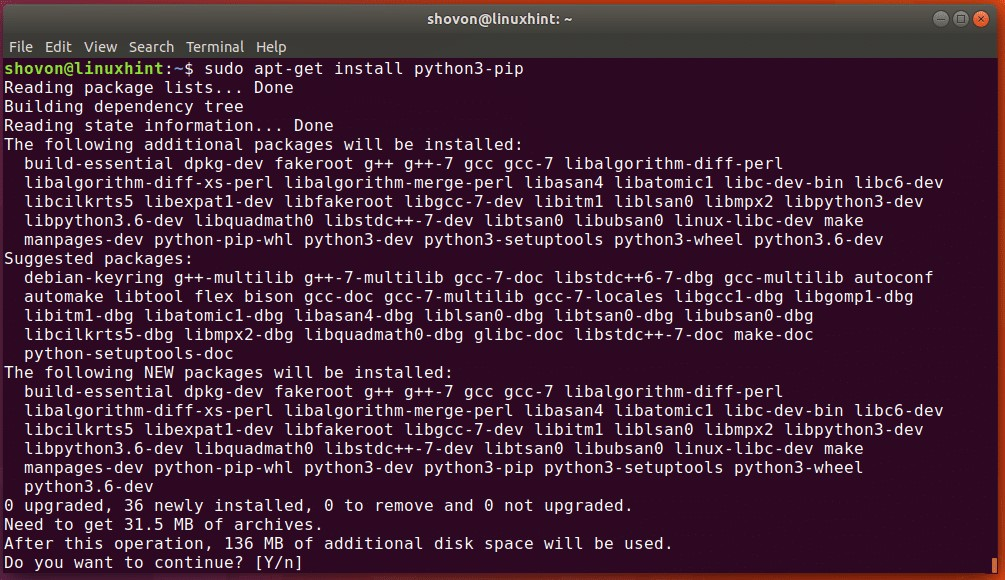
\includegraphics[width=1\textwidth]{../figures/1aptinstal.jpg} 
\caption{sudo apt-get update}
\label{instal}
\end{center}
\end{figure}
Pada Gambar \ref{instal} menjelaskan tentang proses melakukan instalasi pyhton.
\item Verifikasi PIP \\
Proses ini untuk menverifikasi apakah pip dan semua dependensi sudah terinstal atau belum agar dapat berjalan dengan optimal.\\
\begin{figure}[h]
\begin{center}
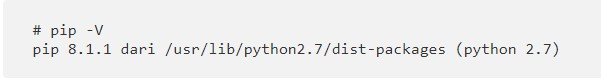
\includegraphics[width=1\textwidth]{../figures/1aptver.jpg} 
\caption{Pip -V}
\label{versi}
\end{center}
\end{figure}

Pada Gambar \ref{versi} menjelaskan tentang untuk menunjukkan versi pip yang telah diinstal.
\subsection{Instalasi PIP di Linux}
Pada umumnya perangkat python merupakan perangkat lunak yang termasuk di dalam disribusi Linux. Untuk linux distribusi slackware digunakan Python versi 2.4, yang terdapat pada CD I direktori/slackware/d. Menggunakan Toolkit untuk melakukan installasi paket di slackware adalah installpkg, berikut langkah instalasinya.\\
\item  mount/mnt/cdrom\\
\item  cd/mnt/cdrom/slackware/d\\
\item  installpkg python-2.4.1-i486-1tgz\\
\\
Python adalah menyediakan modus interaktif yang sangat berguna dalam melakukan latihan dan tes kode. Untuk menulis kode dalam modus interaktif dilakukan dengan memanggil toolkit python pada shell Linux. \\
\item  python\\
\item Python 2.4.1 (1, Apr 10 2005, 22:30:36) \\
\item GCC 3.3.5 on linux2 \\
\item Type "help", "copyright", "credits" or "license" \\
\item for more information.\\
\item  >>>\\
 Tanda “>>>” merupakan suatu prompt dalam modus interaktif Python, selanjutnya Python siap menerima input kode yang dimasukkan.\\

\section{Perintah Dasar PIP}
\subsection{Perintah Bantuan dalam PIP}
Berikut beberapa fungsi yang dapat membantu pengguna ketika dalam menggunakan PIP, antara lain :
\subsubsection{Help}
\begin{figure}[h]
\begin{center}
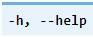
\includegraphics[width=1\textwidth]{../figures/1help.jpg}
\caption{Fungsi Help}
\label{FungsiHelp}
\end{center}
\end{figure}
Pada Gambar \ref{FungsiHelp} menjelaskan bahwa salah satu fungsi dalam PIP yang dapat menunjukkan bantuan.
\subsubsection{Version}
\begin{figure}[h]
\begin{center}
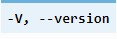
\includegraphics[width=1\textwidth]{../figures/1versi.jpg} 
\caption{Fungsi Version}
\label{fungsiversi}
\end{center}
\end{figure}
Pada Gambar \ref{fungsiversi} menjelaskan tentang salah satu fungsi pada PIP yang dapat menunjukkan versi PIP yang kita gunakan.
\subsubsection{Cache}
\begin{figure}[h]
\begin{center}
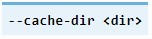
\includegraphics[width=1\textwidth]{../figures/1cache.jpg} 
\caption{Fungsi cache}
\label{fungsicache}
\end{center}
\end{figure}
Pada Gambar \ref{fungsicache} menjelaskan tentang salah satu fungsi pada PIP yang dapat mmenyimpan data cache ke direktori %<dir>
\subsubsection{No Cache}
\begin{figure}[h]
\begin{center}
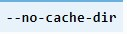
\includegraphics[width=1\textwidth]{../figures/1nocache.jpg} 
\caption{Fungsi NoCache}
\label{fungsinocache}
\end{center}
\end{figure}
Pada Gambar \ref{fungsinocache} menjelaskan tentang salah satu fungsi pada PIP untuk menonaktifkan cache
\subsection{Dasar PIP}
Ada beberapa aturan dalam menangani penggunaan string python yang dapat diandalkan :
\item Tanda kutip tunggal (') atau tanda kuutip ganda (")
\item Apabila dalam penggunaan suatu string terdapat karakter kutip tunggal (') penulisannya diapit kutip ganda (")
\item Apabila dalam penggunaan suatu string terdapat karakter kutip tunggal (") penulisannya diapit kutip ganda (')
\subsection{Perintah Dasar PIP}
Ada beberapa sintaks dasar dalam pemrograman python.
1.	Insialisasi variable. Inisialisasi variable atau statement penugasan adalah sintaks dasar dalam python, contohnya a = 2. Angka 2 adalah identitas dari variable a. Selain itu, ada juga yang dinamakan statement multi baris yang ditandai dengan beberapa baris yang terdapat symbol slash (/"). Ada pula yang dinamakan statement tanda kurung '[]','{}','()" tanpa ada slash (/")
2.	Baris dan indentasi. Kode blok yang digunakan di python menggunakan spasi (indentasi). Jumlah spasi setiap baris yang ada dalam satu blok harus sama dan sesuai.
3.	Tanda kutip dalam python. Python menggunakan tanda kutip ('), (""), ('"), ("") untuk menandai string.
4.	Komentar di python. Tidak seperti Bahasa pemrograman lain yang umumnya menandai komentar denga symbol backslash (\"). Di pemrograman python, komentar di tanadi denga symbol tetagar (\#).
\subsection{Perintah Dasar PIP}
Perintah-perintah dasar pip
Disini saya akan menjelaskan tentang instalasi package
1.	Untuk perintah instalasi package menggunakan perintah $pip install <nama-package>
2.	Bisa menambahkan versi sesuai yang diinginkan dibelakangnya contohnya $pip install <nama-package>=2.0.1
3.	Sebagai contohnya, disini akan menginstal pafy dengan menggunakan perintah $ pip install pafy
4.	Lalu uji dengan perintah $python -c import pafy
5.	Dan selesai..

\section{Contoh Penggunaan PIP}
\subsection{Contoh penggunaan PIP} 
Contoh Pengguaan pip dalam Proses enkripsi dan deskripsi suatu file dengan algoritma Huffman di implementasikan dalam bahasa python.
\item	Fungsi main
Digunakan perintah python [compress/decompress] [filename] untuk argumen “compress” untuk mengenkripsi dan memampatkan file dan argumen decompress untuk membuka kembali menjadi file.
\item	Fungsi ENCODE
Hasil file yang di enkripsi adalah Namafile+’Compressed.txt’.
\item	Fungsi DECODE
Hasil file adalah NamaFile + ’decompressed.txt’.
\subsection{Contoh penggunaan PIP}
Kita dapat melakukan install package-package yang dibundel dengan file berekstensi whl melalui PIP,wheel adalah format arsip yang digunakan untuk mempercepat melakukan penginstalan package. Setelah melakukan penginstalan wheel, lakukan penginstalan paket dengan menggunakan perintah pip install nipype-0.10.0-py2-none-any.whl . Untuk menampilkan package-package yang telah di install gunakan perintah pip list dan untuk menguninstall package lakukan dengan perintah pip uninstall <nama-package>.
\subsection{Instalasi Package Sekaligus}
Pada PIP, kita dapat melakukan penginstalan package sekaligus lebih dari satu package dan  kita tdiak perlu repot untuk menginstal satu per satu package. Pada PIP, untuk menginstal package sekaligus menggunakan requirement.txt, dimana kita melakukan list package yang akan di list dan dimasukkan dalam requirement.txt tersebut. Lalu kita ketikkan perintah
\begin{figure}[h]
\begin{center}
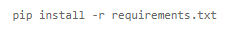
\includegraphics[width=1\textwidth]{../figures/1requre.png}
\caption{Perintah Instal Package Sekaligus}
\label{1require} 
\end{center}
\end{figure}
Pada gambar \ref{1require} menjelaskan tentang bagaimana cara instal package sekaligus dalam satu waktu.
\end{itemize}
\subsection{Contoh Penggunaan PIP}
Contoh penggunaan PIP;
PIP atau biasa dikenal dengan Python Index Packaging dapat dijalankan di berbagai Operating System, di antaranya : System Linux/Unix, Windows, Mac OS X, Java Virtual Machine, OS/2, Amiga, Palm, dan Symbian. Dalam penggunaannya, PIP sangat cocok untuk developing aplikasi berbasis WEB, Developing aplikasi berbasis GUI, Game Developing baik di computer atau mobile, dan masih banyak lagi.
\subsection{Contoh Penggunaan PIP}
Contoh penggunaan PIP;\\
A. Instalasi kebutuhan server
Tahap ini membutuhkan library python dan beberapa modul library python yang diperlukan untuk mempermudah proses development program.\\
1.Update repository\\
Dilakukan update dengan cara apt-get update\\
2. instalasi library python\\
apt-get install python-dev python-setuptools python-pip mongodb gcc\\
3. instalasi library python\\
pip install –r requirements.txt
\subsection{Contoh Pemanfaatan PIP}
Pemanfaatan Raspberry Pi untuk Hacking dan Forensic dengan metode NIST (National Institute of Standards and Technology)
Cybercrime dilakukan oleh orang yang tidak bertanggung jawab dengan tujuan merusak, memodifikasi dan menghilangkan data seseorang, salah satunya dengan menggunakan teknik hacking untuk masuk kedalam sebuah penyimpanan data untuk melakukan kejahatan.  Maka penelitian yang dilakukan adalah melakukan analisis terhadap bukti digital pada jaringan berbentuk pcap dan bukti elektronik berupa flashdisck sebagai media penyimpanan, dengan memanfaatkan Raspberry pi dan NIST.
\subsection{Contoh Pemanfaatan PIP}
Salah satu manfaat Rasberry Pi adalah bisa digunakan sebagai Mini PC untuk controlling dan monitoring suatu perangkat. Salah satu fungsi Raspberry Pi, yakni web server memanfaatkan fitur GPIO (General Purpose Input Output) pada Raspberry Pi. Berkat pemanfaatan ini, setiap perangkat elektronik di rumah dapat di control. Untuk mengontrolnya, menggunakan komunikasi pengontrolan web server melalui protocol TCP/IP serta HTTP.
\end{document}

\chapter[Variabel]
{Variabel}











/Section{Pengertian Variabel}
Variable adalah suatu objek penelitian yang bervariasi dan memiliki gejala yang 
bervariasi, atau sebagai suatu pusat penelitian yang dapat diukur. Variable juga 
sebagai konsep yang mempunyai  lebih dari satu nilai , suatu keadaan dan suatu kondisi.
Pembahasan tentang variable sangat  penting  untuk suatu keperluan pada penetapan system
penelitian, menstrukturkannya ke dalam teori penelitian sebagai landasan pengembangan 
hipotesis .  


\chapter[Penjelasan JSON dan YAML]
{Penjelasan JSON dan YAML}
\documentclass[a4paper]{article}
\usepackage{graphicx}
\begin{document}
\section{JSON}
\subsection{Definisi JSON}
JSON atau JavaScript Object Notation adalah salah satu bentuk format yang ringkas untuk melakukan pertukaran sebuah data di dalam computer. JSON sendiri berbasis teks dan mudah untuk dibaca oleh manusia serta dapat digunakan untuk representasi struktur data sederhana JSON juga dapat digunakan untuk proses transmisi data terstruktur melalui media koneksi jaringan yang disebut Serialisasi.
\subsection{Definisi JSON}
JSON  adalah  bagian  dari  sebuah bahasa  pemrograman  JavaScript  JSON juga merupakan format teks yang sepenuhnya independen tetapi menggunakan konvensi yang  familiar  dengan  bahasa  pemrograman  dari  parent-C,  termasuk  bahasa C,  Java,  Java Script,  Perl, Python,  dan lain sebagainya.  Kelebihan  inilah  yang  membuat  JSON  menjadi  sebuah  bahasa yang disebut  data-interchange yang ideal.
\subsection{Struktur pada JSON}
JSON memiliki 2 struktur,yaitu:
1.	Kumpulan pasangan nama/nilai.
Dalam beberapa Bahasa pemrograman, ini biasanya sering disebut seperti objek, rekaman, struktur, kamus, tabel hash, daftar berkunci atau array assosiatif.
2.	Daftar nilai terurutkan.
Dalam kebanyakan Bahasa pemrograman, ini biasanya sering disebut seperti array, vektor, daftar, atau urutan.
Struktur data tersebut sering kali disebut sebagai struktur data universal. Semua bahasa pemrograman modern mendukung struktur data tersebut dalam bentuk yang sama maupun berbeda.
\subsection{Pengertian Lain Dari JSON}
JSON atau biasa dilafalkan dengan “Jason” merupakan singkatan dari JavaScript Object Notation adalah suatu format ringkas pertukaran data computer. Format Json berbasis teks dan mudah dibaca-manusia serta digunakan untuk merepresentasikan struktur data sederhana dan larik asosiatif. JSON juga seringkali digunakan untuk transmisi datayang  terstruktur melalui suatu koneksi jaringan pada suatu proses yang disebut serialisasi.

\section{YAML}
\subsection{Definisi YAML}
YAML atau YAML Ain't Markup Language adalah sebuah standar yang sudah umum untuk digunakan proses Serialisasi data dalam semua Bahasa pemrograman. YAML dapat memberikan representasi data dengan bentuk yang lebih sederhana. Salah satu bentuk penyederhanaan nya adalah dengan menghilangkan tanda {} dan tanda []. YAML sendiri juga memiliki fitur yang tidak dimiliki oleh JSON.
\begin{figure}[ht]
\centerline{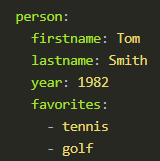
\includegraphics[scale=1]{../figures/5SC.png} }

\caption{Contoh Source Code} 
\label{Sc}
\end{figure}

Pada gambar \ref{Sc} dijelaskan tentang Contoh Source Code.

\subsection{Definisi Lain dari YAML}
YAML merupakan format serial data yang dapat dibaca oleh manusia yang mengambil beberapa bahas apemrograman seperti XML, C, Python, serta format email seperti yang recantum dalam RFC 2822. Pengusul YAML adalah Clark Evans pada tahun2001 silam. Clark merancang format ini bersama dengan Ingy döt Net dan Oren Ben-Kiki. YAML pula tersedia dalam beberapa Bahasa dan script pemrograman.
\subsection{YAML}
YAML mengintegrasikan dan membangun berdasarkan konsep yang dijelaskan oleh bahasa C, Java, Perl, Python, Ruby, RFC0822 (MAIL), RFC1866 (HTML),RFC2045 (MIME), RFC2396 (URI), XML, SAX, SOAP, dan JSON.
Sintaks YAML motivated oleh Internet Mail (RFC0822) dan tetap sebagian kompatibel dengan standar itu. selanjutnya, meminjam dari MIME (RFC2045), produksi tingkat atas YAML adalah aliran dokumen independen, ideal untuk pesan berbasissistem pemrosesan terdistribusi.
\subsection{Definisi YAML}
Pada saat awal-awal perkembangan, YAML diartikan dari banyak orang adalah sebuah singkatan yaitu "Yet Another Markup Language". Namun seiring berkembangnya zaman, untuk memberitahu tujuannya lebih jauh yang terfokus pada data dan bukan markah dokumen, akhirnya singkatan YAML diubah menjadi "YAML Ain't a Markup Language." YAML tersedia untuk beberapa Bahasa dan skrip pemrograman.
\subsection{YAML}
Dari pembahasan di atas, yang telah membahas tentang JSON atau JavaScript Object Notation dan YAML atau YAML Aint Markup Language. Berdasarkan pembahasan di atas dapat di temukan perbedaan antara keduanya. Berikut adalah beberapa perbedaan yang dapat kami kemukakan :
Berikut adalah tabel \ref{table:perbedaan} perbedaan JSON dan YAML.
\begin{table}[h]
\caption{Perbedaan JSON dan YAML}

\centering
\begin{tabular}{ccc}
\hline
&JSON&YAML\\
\hline
Kegunaan&Cocok untuk Format Serialisasi&Cocok untuk konfigurasi\\
\hline
Fitur&tidak memiliki komentar, aliasing&memiliki komentar, aliasing \\
&dan anchoring, dan  mergering& dan anchoring, dan  mergering\\
\hline
\end{tabular}
\label{table:perbedaan}
\end{table}

\end{document}


\chapter[Fungsi Python]
{Fungsi Python}
\documentclass[12pt,a4paper]{article}
\usepackage[left=3.00cm, right=2.00cm, bottom=2.00cm, top=3.00cm]{geometry}
\linespread{1.5}
\begin{document}
\title{FUNGSI PYTHON}
\maketitle

\begin{itemize}
\item
NAMA KELOMPOK 4\\
Ajis Trigunawan			1164031\\
Alimu Dzul Ikroom		1164032\\
Muhammad Hanafi			1164092\\
Riki Karnovi			1164052\\
Yoga Sakti Hadi P		1164059\\
\end{itemize}

\section{Fungsi Phyton}
Python adalah bahasa pemrograman yang dibuat oleh Guido van Rossum dan popular sebagai bahasa skripting dan pemrograman Web. Merujuk pengertian dari wikipedia, Python adalah bahasa pemrograman interpretatif multiguna dengan filosofi perancangan yang berfokus pada tingkat keterbacaan kode. Python diketahui sebagai bahasa yang kemampuan dengan sintaksis kode yang sangat jelas. Salah satu fitur yang tersedia pada python adalah sebagai bahasa pemrograman dinamis yang dilengkapi dengan manajemen memori otomatis.\\

Python bisa digunakan dalam bermacam-macam pengembangan perangkat lunak dan juga bisa berjalan di banyak platform sistem operasi. Sebuah Komputer hanya bisa mengeksekusi program yang penulisannya dalam bahasa mesin atau bahasa tingkat rendah. Python adalah salah satu bahasa pemrograman tingkat tinggi, Sehingga agar bisa di eksekusi maka program harus diproses dulu sebelum dapat dijalankan. Keuntungan Python dengan bahasa tingkat tingginya yaitu lebih manusiawi.\\

Bahasa tingkat tinggi bisa dengan mudah dirubah portabel untuk disesuaikan dengan mesin yang menjalankannya. Hal ini beraneka ragam dengan bahasa mesin yang hanya dapat digunakan untuk mesin tersebut. Dengan berbagai macam kelebihan ini, maka tidak sedikit aplikasi ditulis menggunakan bahasa tinflrat tinggi. Proses mengubah dari bentuk bahasa tingkat tinggi ke tingkat lebih kecil dalam bahasa pemrograman ada rkra tipe.Yakni interpreter dan compiler. interpreter membaca program berbahasa tingkat tinggi lau memproses program tersebut. Hal ini berarti interpreter melakukan perintah apa yang dikatakan dalam program tersebut. Dapat dikatakan. interpreter membaca per baris kemudian mengeksekusinya. \\

Python merupakan Bahasa pemograman yang hampir tidak bisa dibedakan dengan C/C++, Setiap python mempunyai fungsi yang dapat mengembalikan sebuah Nilai, Tetapi di Python  bisa juga  tidak mengembalikan sebuah Nilai dan biasaya dikenal dengan nama subroutines yang terdapat pada pemograman VB. Python merupakan Bahasa yang tidak menggunakan compiler dan Bahasa ini juga bisa mengembangkan perangkat lunak, Membangun GUI desktop dan lain-lain.\\

Python dalam pengambangan web sering digunakan dibackend untuk portal pengaksesan database server atau pembuatan API dengan mekanisme Client-Server, selain itu Python juga banyak digunakan untuk mengembangkan AI oleh google dan developer atau perusahaan lainnya. Python juga di gunakan untuk pengembangan jaringan syaraf tiruan salah satunya project tensorflow. Python juga banyak digunakan dalam IOT karna python adalah salah satu bahasa mesin yang mudah dipelajari dan di pahami. Dapat juga digunakan dalam pembuatan atau pengembangan robot pintar, membuat program untuk melakukan konfigurasi jaringan, melakukan Data Minning untuk mendapatkan data yang dibuthkan, dan dapat juga digunakan untuk membuat aplikasi desktop maupun command line.\\

Terkadang ketika membuat suatu program yang kompleks adakalanya kumpulan instruksi dijadikan satu dalam satu berkas, terutama apabila sering menggunakan sekumpulan intruksi untuk melaksanakan satu tugas yang sifatnya rutin. Skrip python ditulis dengan akhiran .py. Setiap Skrip pada python dianggap sebagai modul. Intinya Modul adalah kode yang disimpan dalam sebuah berkas dalam media penyimpan eksternal. Selanjutnya, kode yang terdapat dalam modul dapat dipergunakan dalam suatu skrip dengan terlebih dahulu mengimpor (mengambil) modul tersebut.\\

Di dalam python, objek merupakan abstraksi terhadap data. Setiap data dinyatakan dalam objek. Sebuah objek memiliki nilai dan tipe, misalnya ketika diberikan perintah a=5, maka sebenarnya a adalah objek. Tipenya adalah bilangan bulat dan nilainya adalah 5. Dan yang perlu diketahui begitu diberikan nilai pada suatu objek maka identitas objek tersebut tidak berubah. Identasi (penulisan text yang menjorok ke kanan) memegang peranan penting dalam penulisan pernyataan pada python mengingat identasi digunakan sebagai blok kode pada pernyataan seperti if, while, dan for.\\

Python ialah bahasa pemrograman yang sangat mempunyai fungsi yang baik dan disukai oleh pengguna karena :
\begin{enumerate}

\item Sederhana
Python didirikan berdasarkan prinsip pengkodean yang dikembangkan oleh bahasa sebelumnya, namun prinsip-prinsip ini telah dieksploitasi untuk implementasi yang lebih sederhana dalam pemrograman Python.

\item High Level
Python ialah bahasa pemrograman yang sederhana. Ini bisa digunakan untuk pemrograman fungsi yang paling canggih sampai fungsi paling rendah.

\item Sangat sesuai untuk analisis
 Python banyak digunakan dalam matematika dan sains
 
\item Open Source
Python adalah Bahasa pemrograman yang bersifat open source atau tidak berbayar dapat didownload pada www.python.org secara gratis.\\

\item Bersifat OOP.

Python sangatlah cocok untuk menulis program paralel tingkat tinggi. Python sekarang muncul sebagai alternatif kompetitif yang potensial untuk Matlab, Octave, dan lingkungan serupa lainnya. Keuntungan khusus Python adalah bahasanya sangat kaya dan kuat, terutama jika dibandingkan dengan Matlab, Fortran, dan C. Secara khusus, Python adalah bahasa berorientasi objek yang ditafsirkan yang mendukung operator overloading dan menawarkan antarmuka antar-platform ke operator fungsi sistem. Pemrogram C ++ Canggih dapat dengan mudah mencerminkan desain perangkat lunak mereka dengan Python dan bahkan memperoleh lebih banyak fleksibilitas dan keanggunan.\\

\end{enumerate}

Keuntungan lain dari Python adalah bahwa perangkat lunak warisan antarmuka yang ditulis dalam Fortran, C, dan Tidak ada tahapan kompilasi dan penyambungan (link) sehingga kecepatan perubahan pada masa pembuatan sistem aplikasi meningkat. Lalu C ++ jauh lebih sederhana daripada di sebagian besar lingkungan lainnya. Ini karena Python dirancang untuk dapat diperpanjang dengan kode yang dikompilasi untuk efisiensi, dan beberapa alat tersedia untuk memudahkan integrasi kode Python dan dikompilasi.





\end{document}


\chapter[Hello World Python dan Identation]
{Hello World dan Identation}
%Resume Hello word python dan identation

%Kelompok 2 D4 TI / 2B

%Alwan Suryansah				1164033 
%Dinda Ayu Pratiwi				1164034
%Kurnia Sandi					1164042
%Teduh Sanubari					1164054
%Wildan Khaustara Wijaksana		1164058

\documentclass[12pt]{article}
\usepackage{graphicx}    

\begin{document}
\section{Apa itu Pyton?}

\subsection{Journal JCONES}
	Tulisan ini mendiskusikan pengertian python , python adalah sebuah bahasa pemrograman model skripsi atau ( scripting language) terorientasi objek. atau bisa juga di artikan sebagai bahasa pemrograman yang freeware atau perangkat bebas , tidak ada batasan dalam penyalinan atau mendistribusikan . yang di dalamnya terdapat source code , debugger dan profiler \cite{perkasa2014rancang}.
	
\subsection{Dierbach, Charles}
Bahasa pemrograman Python telah dengan cepat mendapatkan popularitas selama beberapa tahun terakhir sebagai bahasa pilihan untuk kursus CS1. Beberapa perkiraan menyebutkan bahwa penggunaannya meningkat empat puluh persen per tahun. Sejauh 2006 ada laporan peningkatan yang signifikan dalam kepuasan siswa dan instruktur dengan mendesain ulang kursus pengantar untuk menggunakan kesederhanaan Python daripada kompleksitas bahasa seperti Java\cite{dierbach2014python}.

\subsection{Computing, Jurnal ULTIMA}
Python merupakan bahasa pemrograman open source yang banyak digunakan untuk menangani beberapa jenis masalah dalam pemrograman. Python banyak digunakan untuk meningkatkan kualitas perangkat lunak, produktivitas pengembang, portabilitas program, dan integrasi komponen. Python digunakan oleh setidaknya ratusan ribu pengembang di seluruh dunia dalam bidang-bidang seperti scripting internet, pemrograman sistem, user interface, kustomisasi produk, pemrograman numerik, dan banyak lagi\cite{computingaplikasi}.

\subsection{Herho, Sandy Hardian Susanto}
Python merupakan bahasa pemrograman tingkat tinggi yang dewasa ini telah menjadi standar dalam dunia komputasi ilmiah. Python merupakan bahasa pemrograman open source multi-platform yang dapat digunakan pada berbagai macam sistem operasi (Windows, Linux, dan MacOS). Selain itu, Python juga merupakan bahasa pemrograman yang fleksibel dan mudah untuk dipelajari. Program yang ditulis dalam Python umumnya lebih mudah dibaca dan jauh lebih ringkas dibandingkan penulisan program dalam bahasa C atau Fortran. Python juga memiliki modul standar yang menyediakan sejumlah besar fungsi dan algoritma, untuk menyelesaikan pekerjaan seperti mengurai data teks, memanipulasi dan menemukan file dalam disk, membaca / menuliskan file terkompresi, dan mengunduh data dari server web. Dengan menggunakan Python, para programmer juga dapat dengan mudah menerapkan teknik komputasi tingkat lanjut, seperti pemrograman berorientasi objek\cite{herho2018tutorial}.

\subsection{Rizky, Gusti Yudhistira and Anbarsanti, Nurfitri and others}
Bahasa python sendiri adalah Bahasa pemrograman yang bersifat freeware. Maksudnya adalah tidak memiliki batasan dalam melakukan penyalinan atau pemakaiannya yang lengkap dengan source codenya, debugger, dan profiler, interface service, fungsi system GUI, dan basis datanya sehingga dapat membuat python menjadi basaha asli raspberry. Python sendiri memiliki beberapa fitur. Seperti memiliki kepustakaan yang luas dengan modul-modul siap pakai untuk berbagai macam keperluan\cite{rizky2016desain}. 

\section{Membuat "Hello World" dengan Pyton}
"Hello World" adalah kalimat sakral yang pertama kali dimunculkan menggunakan bahasa pemrograman tertentu dalam sistem. Para coder dari tahap beginner hingga tingkat expert pun pasti hal yang pertama ia lakukan adalah memunculkan "Hello World" di sistem. Karena prinsip utama dalam pemrograman adalah bagaimana memunculkan apa yang kita tulis atau kita buat dengan bahasa pemrograman tertentu ke sebuah layar atau sistem baik dengan atau tanpa data.
Berikut ini adalah code untuk menampilkan "Hello World" di layar menggunakan bahasa pemrograman Python

\begin{verbatim}
>>> print('hello world')
hello world
\end{verbatim}

\subsection{Membuat "Hello World" dengan menggunakan Token pada bahasa Python}
Pada bahasa python terdapat kalimat "Hellow World" di layout awal untuk melihat apakah ada terdapat error pada halaman itu.apa bila tidak terdapat error "Hello World" akan muncul di halaman awan atau layout awal . dengan menggunakan Token instance mewakili unit teks seperti kata,kalimat, atau dokumen, dan didefinisikan oleh (sebagian)pemetaan dari nama properti kenilai.Sebagai contoh,properti Text digunakan untuk menyandikan token\cite{bird2004nltk}:

\begin{verbatim}
>>> dari nltk.token impor *
>>> Token (TEXT = "Hello World!")
<Hello World!>
\end{verbatim}

Secara umum, tugas pemrosesan bahasa diformulasikan sebagai anotasi dan transformasi yang melibatkan Token. Secara khusus, setiap tugas pemrosesan membutuhkan token dan meluasnya untuk memasukkan informasi baru. Modifikasi ini biasanya monotonik; baru informasi ditambahkan tetapi informasi yang ada tidak dihapus atau diubah. Jadi, token berfungsi sebagai papan tulis, dimana informasi tentang sepotong teks disusun. Arsitektur ini berbeda dengan yang lainnya arsitektur pipa khas di mana setiap pemrosesan keluaran tugas membuang informasi masukannya. Kita memilih pendekatan papan tulis di atas pipa pendekatan karena memungkinkan lebih banyak fleksibilitas kapan menggabungkan tugas ke dalam satu system\cite{bird2004nltk}.

\subsection{Membuat "Hello World" dengan Pyton menurut Perkel, Jeffrey M}
Bahasa pemrograman Python lebih mudah dinyatakan, pengguna tidak harus menentukan variabel mana yang akan menyimpan angka atau teks, misalnya. Latihan pemrograman klasik Percetakan 'Hello, world!' ke layar sesederhana mungkin dengan Python - ketikkan saja

\begin{verbatim}
print ("Hello, world!”)
\end{verbatim}
pada prompt Python dan tekan Enter\cite{perkel2015programming}.

\subsection{Membuat "Hello World" Menurut Buku Logika algoritma dan implementasinya dlm bahasa python di gnu/linux}
Python merupakan salah satu bahasa pemrograman tingkat tinggi dengan tipe bahasa interpreted karena program-program Python langsung dieksekusi oleh interpreter tanpa harus melalui tahap kompilasi. Python dapat dijalankan dengan dua cara, yakni:
\begin{enumerate}
\item Mode command-line
Dengan mode ini, program dapat dilakukan dengan memanggil interpreter, kemudian memberi statement Python dan interpreter akan menampilkan hasil, sebagai contoh:
\begin{verbatim}
bash-2.05a$ python
Python 2.1.3 (#1, Apr 20 2002, 10:14:34)
[GCC 2.95.4 20011002 (Debian prerelease)] 
on linux2 Type "copyright", "credits" or 
"licence" for more information.

>>> print 1+1
2
>>> print "Hello World!"
Hello World!
\end{verbatim}

\item Mode Script
Mode ini dilakukan dengan cara menuliskan keseluruhan program dalam file, kemudian interpreter akan mengeksekusi seluruh isi dari file. File seperti ini dinamakan script. Sebagai contoh, sebuah file yang ditulis dengan text editor dan diberi nama script01.py memiliki isi sebagai berikut:
\begin{verbatim}
print 1+1
\end{verbatim}
Dengan perjanjian bahwa file yang berisi program Python diberi nama dengan ekstensi .py. Eksekusi dari program dengan mode ini dapat dilakukan dengan cara sebagai berikut:
\begin{verbatim}
$ python script01.py
2
Contoh 1:
# -------------------
# Program Sederhana
# by Ema dan Wawan
# -------------------
print "I Like Python"

Contoh 1.1:
# -------------------
# Program Sederhana
# by Kurnia Sandi
# -------------------

print "Hello World!"
\end{verbatim}
Catatan: Python tidak membutuhkan titik koma (semicolon) di belakang statement. Semicolon di sini sifatnya optional sehingga bisa digunakan, tetapi juga boleh tidak dipakai\cite{utami2004logika}.
\end{enumerate}

\subsection{Membuat "Hello World" Menurut Gario, Marco and Micheli, Andrea}
Python merupakan salah satu bahasa pemrograman tingkat tinggi akan tetapi python memiliki code atau syntax yang singkat , dan menggunakan bahasa C, C++, maupun Java, yakni:


\begin{verbatim}
from pysmt.shortcuts import * 
from pysmt.typing import INT 
 hello = [Symbol(s, INT) for s in "hello"] 
 world = [Symbol(s, INT) for s in "world"] 
 letters = set(hello+world) 
 domains = And([And(GE(l, Int(1)), 
 LT(l, Int(10))) for l in letters]) 
 sum_hello = Plus(hello) # n-ary operators can take lists 
 sum_world = Plus(world) # as arguments 
 problem = And(Equals(sum_hello , sum_world),
 					Equals(sum_hello , Int(25))) 
 formula = And(domains , problem) 
 print("hello world:") 
 print(World) 
 
 model = get_model(world , solver_name="z3") # Try msat 
 
 if model: print(model) 
 else: print("No solution found")

\end{verbatim}

\subsection{Menyapa Program Hello World Menurut Sweigart, Al}
Itu tradisional bagi pemrogram untuk membuat tampilan pertama mereka Hello World! di layar. Anda akan membuat program Hello World Anda sendiri sekarang\cite{sweigart2016invent}.
\begin{verbatim}
1. # Program ini menyapa dan menanyakan nama saya.
2. print('Hello world!')
3. print('Siapa nama Anda?')
4. myName = input ()
5. print('Ini baik untuk bertemu dengan Anda,' + myName)
\end{verbatim}

\subsection{Menyapa Program Hello World di CMD menurut Kurniawan, Agus}
Dibawah ini merupakan fungsi Python yang digunakan untuk menampilkan atau mencetak. ada bahsa pemrograman Python untuk mencetak gunakan fungsiprint() , dimana yang kita cetak harus berada di dalam buka kurung da tutup kurung tersebut ,.

Jika ingin mencetak tipe data String , kita harus memasukanya kedalam tanda kutip terlebih dahulu
Pertama anda pastikan Program Pythonnya berjalan dan cek versinya:\cite{kurniawan2016getting}.

\begin{verbatim}
C:\>python
ActivePython 3.3.4.1 (ActiveState Software Inc.) based on
Python 3.3.4 (default, Feb 25 2014, 15:11:05) [MSC v.1600 32 bit (Intel)] on win
32
Type “help”, “copyright”, “credits” or “license” for more information.
>>>print("Hello World")

\end{verbatim}

\subsection{Sochat, Vanessa}
Misalnya, untuk mengetahui lokasi eksak yang tepat yang ditulis dalam program yang berbeda bahasa ming untuk menghasilkan output "Hello World," kita bisa lakukan pembanding lebih lanjut dengan isinya, atau lakukan panggilan bahasa agnostik dengan melakukan atrace of system calls. Maka dari itu jenis penilaian yang memungkinkan untuk organisasi aplikasi dan aksesibilitas adalah hal yang terpenting\cite{sochat2018scientific}.

\subsection{Parra, Alfredo}
Seperti gambar pada di bawah ini untuk memunculkan "Hello World" pada scrip python.


\begin{figure}[ht]
\centerline{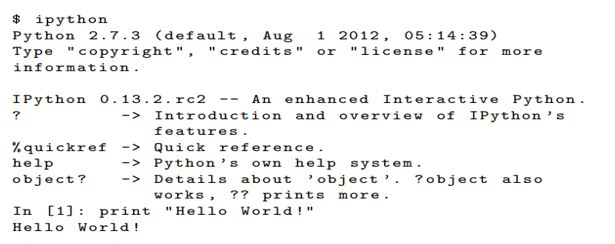
\includegraphics[width=1\textwidth]{coding.JPG}}
\caption{Contoh Program Python Hello World}
\label{gambarHWI1}
\end{figure}

Keterangan:
\begin{enumerate}
\item Kerangka interaktif yang disempurnakan.
\item menggunakan python versi 2.7.3.
\item (?) adalah introduction dan overview di python features.
\item quickref untuk quick references .
\item help berfungsi untuk system help dalam python .
\item in [1]: print "hello world!" adalah yang akan muncul di layout sesuai yang di tuliskan.
\item hello world adalah loyout yang muncul setelah di ketikkan di kodingan menggunakan bahasa python.
\end{enumerate}

Pada gambar \ref{gambarHWI1} digunakan untuk memunculkan "Hello World" pada script python\cite{parra2017scripting}.

\subsection{Hello World Fangohr, Hans}
Masih banyak kode yang masih digunakan yang ditulis untuk Python 2, dan sangat berguna untuk mengetahui perbedaannya. Contoh yang paling menonjol adalah bahwa dalam Python 2.x, perintahnya istimewa, sedangkan pada Python 3 itu adalah fungsi biasa. Misalnya, dengan Python 2.7, kita dapat menulis:
\begin{verbatim}
print "Hello World"
\end{verbatim}
dimana seperti pada Python 3, ini akan menyebabkan SyntaxError. Cara yang benar untuk menggunakan cetak dengan Python 3 akan menjadi fungsi, yaitu:
\begin{verbatim}
In [1]: print("Hello World")
Hello World
\end{verbatim}
\cite{fangohr2015python}

\subsection{Aplikasi Complite Menurut Grinberg, Miguel}
Versi kedua dari aplikasi, menambahkan rute kedua yang dinamis. ketika Anda mengunjungi URL dinamis di browser Anda, Anda terikat dengan ucapan pribadi yang menyertakan nama yang diberikan di URL.

hello.py: Aplikasi Flask lengkap
\begin{verbatim}
from flask import Flask
app = Flask(__name__)

@app.route('/'0
def index():
return '<h1>Hello World!</h1>'
\end{verbatim}
\cite{grinberg2018flask}
 
\section{Pengertian Identation pada Pyton}

\subsection{Barry, Paul}
Python menggunakan prinsip yang berbeda. Program Python terstruktur melalui indentasi, yaitu blok kode ditentukan oleh indentasinya. Oke, itulah yang kami harapkan dari kode program apa pun, bukan? Ya, tetapi dalam kasus Python itu adalah persyaratan bahasa bukan masalah gaya. Prinsip ini membuatnya lebih mudah untuk membaca dan memahami kode Python orang lain \cite{barry2016head}.

\subsection{Kurniawan, Halim and Setiyono, Budi and Isnanto, R Rizal}
Bahasa pemograman Python adalah bahasa pemograman yang mudah dibaca dan terstruktur, hal ini karena di gunakannya sistem identasi. Yaitu memisahkan blok - blok program susunan identasi. Jadi untuk memasukan sub - sub program dalam suatu blok, sub - sub program tersebut diletakkan satu atau lebih spasi dari kolom suatu blok program itu \cite{kurniawan2011aplikasi}.

\subsection{Burt, Simon}
penyorotan sintaks dalam fitur indentasi khusus untuk Python, Tidak seperti kebanyakan Halnya yang Ada di dalam bahasa pemrograman, Python tidak biasa dalam hal itu menggunakan indentasi, berdasarkan sintaks yang di gunakan untuk membatasi blok kode. Pemrogram ini akrab dengan bahasa lain yang menggunakan delimiter, seperti kurung kurawal {and} untuk mengidentifikasi blok baru dan mungkin akan menemukan kebingungan ini pada awalnya, tetapi dengan cepat menjadi normal\cite{burtusing}.

\subsection{MUTHOA, MUHAMMAD FARIS}
Bahasa pemograman Python yaitu bahasa pemograman yang mudah dibaca dan terstruktur, karena dalam Python digunakannya sistem indentasi/spasi yaitu memisahkan blok-blok program dengan susunan indentasi/spasi. Python sendiri memiliki sedikit perbedaan cara penulisan kode program dengan bahasa pemrograman lainnya, yakni di Python kita hanya menggunakan spasi sebagai pemisah blok program yang biasa disebut sebagai Indentasi. Kalau pada bahasa pemrograman yang lain seperti C/Java menggunakan tanda kurung sebagai pemisah blok program\cite{muthoa2017sistem}.

\subsection{Miftakhuddin, Mukhammad and Suadi, Wahyu and Pratomo, Baskoro Adi}
Identation Yaitu adalah memisahkan blok `blok program susunan identasi. Jadi untuk memasukan sub -sub program ke dalam suatu blok, sub sub program tersebut diletakkan satu atau lebih spasi dari kolom suatu blok program(tulisan yang menjorok kearah kanan. hal ini karena digunakannya sistem indentasi, identasi digunakan sebagai blok kode pada pernyataan seperti if, while, dan for\cite{miftakhuddinimplementasi}. 

\subsection{Kristjan, Arumae and Sarah, Myhre and Cassian, Olschewski}
Indentasi seperti lekukan ekspresi yang bersarang, merupakan hal penting dalam memproduksi skrip Python yang terbaca. Persyaratan indentasi yang ditegakkan Python secara khusus mengurangi ruang untuk kesalahan saat pengembang bekerja dengan basis kode tertentu. Selanjutnya, persyaratan dalam membuat kode yang dihasilkan umumnya lebih mudah dibaca dan dengan demikian lebih mudah dipelihara\cite{kristjansoccer}.


\section{Error yang Muncul serta Solusinya}
\subsection{Perintah If}
Perintah if digunakan untuk menangani permasalahan bersyarat. Berikut ini contohnya:
\begin{verbatim}
>>> x = 12014081
>>> if x > 12014081:
... print "NIM di atas Icha."
... elif x <12014081:
... print "NIM di bawah Icha."
... else:
... print "Halo, Icha!"
...
Halo, Icha!
\end{verbatim}

Perhatikanlah bahwa baris pertama dalam rangkaian ini diawali dengan perintah if yang berarti jika, baris kedua dengan perintah elif yang berarti selain “if” (else if), rangkaian diakhiri dengan perintah else yang berarti selain keduanya. Masing – masing perintah ini diakhiri dengan tanda titik dua yang kemudian diikuti subperintah yang hendak dieksekusi. Pada rangkaian perintah if, kedua perintah elif dan else bersifat opsional.

Satu lagi konsep penting dalam pemrograman Python yang harus kalian ingat adalah bahwa spasi dan indentasi mempunyai makna sintaktis. Spasi dan indentasi mendikte bagaimana kita mengeksekusi perintah. Tanda titik dua diperlukan untuk menandai subperintah sesudah perintah if, pada pengulangan (looping), atau sesudah pendefinisan fungsi. Dalam Python, seluruh subperintah yang satu kelompok sesudah tanda titik dua harus memilki indentasi yang sama, jika tidak maka akan menghasilkan error. Untuk lebih jelasnya perhatikan contoh berikut ini:

\begin{verbatim}
>>> if 1 < 3:
... print "baris satu"
... print "baris dua"
File "<stdin>", line 3
print "baris dua"
^
IndentationError: unexpected indent
\end{verbatim}

Coba kalian perhatikan perbedaan contoh tadi dengan contoh berikut ini:

\begin{verbatim}
>>> if 1 < 3:
... print "baris satu"
... print "baris dua"
...
baris satu
baris dua
\end{verbatim}

\section{Kesimpulan}
	Dari berbagai pengertian mengenai bahasa pemograman python kita dapat simpulkan bahwa bahasa pemograman Python merupakan bahasa pemrograman open source yang banyak digunakan untuk menangani beberapa jenis masalah dalam pemrograman. Python banyak digunakan untuk meningkatkan kualitas perangkat lunak, produktivitas pengembang, portabilitas program, dan integrasi komponen\cite{computingaplikasi}.
	
	Didalam Bahasa pemograman Python juga terdapat sistem identasi yang berguna untuk memisahkan blok - blok program susunan identasi. Jadi untuk memasukan sub - sub program dalam suatu blok, sub - sub program tersebut diletakkan satu atau lebih spasi dari kolom suatu blok\cite{kurniawan2011aplikasi}.
	
	
\end{document}




\chapter[3postmandanswagger]
{postmandanswagger}

\documentclass[12pt,a4paper]{article}
\usepackage[left=3.00cm, right=2.00cm, bottom=2.00cm, top=3.00cm]{geometry}
\usepackage{graphics}
\begin{document}
\title{Postman dan Swagger}
\maketitle
\begin{enumerate}
\item Fransiscus Ivan Martongam      1164039 \\
\item Lalita Chandiany Adiputri      1164043\\
\item Eko Cahyono Putro              1164035\\
\item Lidwina Triniska Gulo          1164044\\
\item Sulpadianti Bunyamin           1164096\\
\end{enumerate}

\section{Pengertian Postman}
Postman merupakan sebuah software yang memuat fungsi lengkap pengembangan sistem dalam mengirimkan dan menerima respon server. Software ini mendukung pengembangan sistem REST API dengan mengklasifikasi request berdasarkan request method, URL dan parameter-parameter request. Postman juga adalah sebuah aplikasi (berupa plugin) untuk browser chrome, fungsinya adalah sebagai REST Client atau istilahnya adalah aplikasi yang digunakan untuk melakukan uji coba REST API yang telah kita buat.

\section{Fungsi dari postman}
Menurut Arianto M A, DKK(2016), Sebuah aplikasi yang digunakan untuk melakukan uji coba REST API yang telah kita buat. Fungsi Postman adalah untuk pengecekan web service. Postman dapat menampilkan hasil dari HTTP request yang kompleks sekalipun dengan cepat. Postman muncul sebagai add-on dari chrome namun sekarang sudah menjadi aplikasi native. Postman memudahkan untuk menguji, mengembangkan dan API (Application Programmin Interface) dokumen dengan memungkinkan pengguna untuk dengan cepat mengumpulkan baik permintaan HTTP sederhana dan kompleks

\section{cara instal postman}
Postman for Chrome (aplikasi Postman sebelumnya merupakan ekstensi Chrome App atau aplikasi yang menginduk pada Chrome).
Cara menginstal Postman untuk menginstal Postman versi native pada sistem operasi Ubuntu/Debian yaitu 
Buka terminal lalu unduh atau donwload paket instalasi Postman dengan mengunakan perintah wge,
kemudia Ekstrak file instalasi Postman tersebut ke direktori /optsudo tar -xzf postman.tar.gz -C /opt.
setelah itu dapat menghapus file instalasinya (opsional)dengan cara rm postman.tar.gz


\section{membuat shortcut Postman}
Berikut tata cara untuk membuat shortcut pada start menu postman.  Ketik perintah - perintah berikut dibawah ini:
cat > ~/.local/share/applications/postman.desktop <<EOL
[Desktop Entry]
Encoding=UTF-8
Name=Postman
Exec=postman
Icon=/opt/Postman/resources/app/assets/icon.png
Terminal=false
Type=Application
Categories=Development;
EOL

Sekarang untuk membuka aplikasi yang ada pada Postman , cukup hanya dengan melakukan klik pada shortcut pada start - menu. 

\section{Cara Penggunaan Postman}
Berikut cara penggunaan Postman : Buat sebuah file baru pada direktori root webserver dengan nama: contoh-api-sederhana.php .Kemudian ketikan kode PHP berikut ke dalam file contoh-api-sederhana.php. Berikut kode untuk membuat file:

\begin{figure}[ht]
\centerline{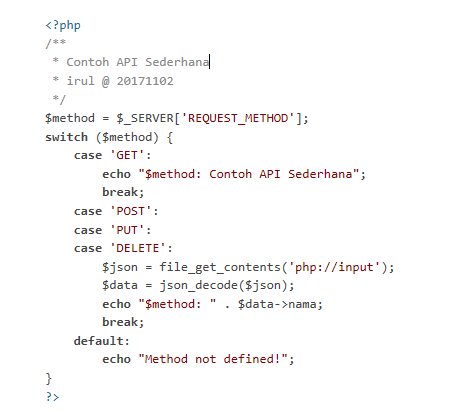
\includegraphics[width=1\textwidth]{figures/3contohapi.PNG}}

\caption{Contoh Api Sederhana} 
\label{api}
\end{figure}

pada gambar \ref{api} menjelaskan tentang contoh api.

Pada file contoh-api-sederhana.php, dapat didefinisikan satu buah API dengan empat Http Request Method yang berbeda. Berikut daftar method dan alamat url yang nanti akan kita uji menggunakan Postman:
•	GET => /contoh-api-sederhana.php
•	POST => /contoh-api-sederhana.php
•	PUT => /contoh-api-sederhana.php
•	DELETE => /contoh-api-sederhana.php
Kita dapat menguji salah satu API di atas menggunakan browser, salah satunya, menggunakan method GET, browser akan mengirimkan data ke server menggunakan method GET.

\section{Implementasi Postman}
Implementasi tidak hanya aktivitas, melainkan suatu kegiatan yang terencana untuk mencapai
tujuan kegiatan. Tahap implementasi pada penelitian ini tidak dilakukan hanya dalam satu proses,
Tetapi dilakukan dalam beberapa sub proses yaitu membangun lingkungan pengembangan sistem, 
mendesain struktur table, function dan stored procedure pada database, mengembangkan sistem back-end (coding) 
dan menyesuaikan dengan database, dan mendesain struktur rewrite pada web server. 

\section{Pengujian}
Untuk memastikan bahwa sistem berjalan sesuai dengan rencana pengembangan sistem dan proses bisnis yang difasilitasi, diperlukan sebuah skenario pengujian sistem. Pada penelitian ini, pengujian akan dilakukan dengan menggunakan software Postman dan dibagi menjadi tiga skenario pengujian, yaitu: Pengujian otentikasi token untuk memastikan prinsip REST terpenuhi, pengujian dengan metode equivalent partitioning untuk memastikan nilai-nilai masukan sesuai dengan rencana pengembangan sistem, pengujian fungsional untuk memastikan setiap titik akses API.

\subsection{Pengujian otentikasi token}
Pengujian  otentikasi token dilakukan pada load-balanced server dengan jumlah back-end server sebanyak tiga virtual server yang diklasifikasi berdasarkan port jaringan. Pengujian  metode equivalent partitioning akan mengelompokkan nilai masukan ke dalam kelas- kelas kemudian diuji dalam kasus-kasus tertentu. Pengujian fungsional dilakukan secara langsung setiap titik akses sistem API yang telah dibuat. 

\subsection {Pengujian dengan metode equivalent partitioning}
Pengujian dengan menggunakan metode equivalent partitioning ini untuk memastikan nilai-nilai masukan sesuai dengan rencana pengembangan sistem. Pengujian ini akan mengelompokkan nilai masukan ke dalam kelaskelas batasan nilai untuk kemudian diuji dalam kasus-kasus tertentu. Rencana pengujian metode ini meliputi validasi path, validasi request method, validasi token, kesesuaian tipe data dan validasi nilai.


\end{document}


\chapter[Instalasi Flask]
{Instalasi Flask}
\documentclass[12pt,a4paper]{article} 
\usepackage{graphicx}
\begin{document}

\section{Flask}
\subsection{Definisi Flask}
Flask merupakan micro web framework yang ditulis dalam bahasa pemrograman Python. Flask disebut micro framework karena tidak membutuhkan tools tertentu. Framework ini juga tidak mempunyai database abstraction layer, validasi form, atau komponen lainnya yang dimana sudah menyediakan library pihak ketiga yang menyediakan fungsi lain. Akan tetapi, framework flask mendukung extension yang dapat menambah fitur aplikasi seakan-akan mereka diimplementasikan dalam flask itu sendiri.
\subsection{Instlasi Flask}
\subsubsection{On Linux}
Untuk melakukan instalasi flask, ada beberapa tahap yang harus dilakukan yaitu :
\begin{enumerate}
\item Pastikan anda sudah menginstal pyhton baik pyhton versi 2.x maupun 3.x. Jika belum instal, instal terlebih dahulu.

\item Untuk melakukan instalasi flask, kita harus membuat sebuah virtual environment lalu instal flask di dalamnya. Berikut adalah cara instal virtual enviroment / virtualenv.

\$ sudo apt-get install python-virtualenv

\item Lalu, buat satu direktori di hard disk kita untuk tempat pengerjaan project. 

\$ mkdir myproject

\$ cd myproject

\item Setelah itu, kita masuk ke direktori yang sudah di buat sebelumnya dan jalankan terminal untuk menjalankan virtualenv untuk membuat virtualenv di dalam direktori tersebut. Berikut adalah cara menjalankan virtualenv.

\$ virtualenv venv

New python executable in venv/bin/python

Installing setuptools, pip............done.

\item Lalu, berikut adalah cara untuk mengaktifkan virtualenv.

\$ . venv/bin/activate 

dan jika ingin menonaktifkannya, berikut caranya 

\$ deactivate

\item Selanjutnya, kita melakukan penginstalan flask

\$ pip install Flask
\end{enumerate}
\subsubsection{On Mac OS}
1. Instal pip terlebih dahulu menggunakan perintah :\\
	python get-pip.py\\

2. Selanjutnya instal flask dengan menggunakan perintah berikut :\\
	sudo pip install Flask\\

3. Sekarang, jalankan Simple.py untuk memastikannya berfungsi dengan menggunakan perintah berikut :\\
	python simple.py\\

Lalu, jalankan di web browser dengan perintah :\\
http://127.0.0.1:5000/

ketika sudah selesai, hentikan server dengan menekan kontrol-C.
\subsubsection{On Windows}
1.	Pertama, bukalah command prompt lalu ketikan perintah: pip install virtualenv
2.	Lalu, buatlah folder untuk aplikasi dengan cara mengetikan perintah: mkdir myproject.
Myproject bisa diganti dengan nama lain sesuai keinginan.
3.	Setelah itu, ketikan perintah untuk masuk ke dalam folder myproject: cd myproject. Lalu ketikan perintah: virtualenv flask
4.	Kemudian, ketikan perintah untuk masuk ke dalam folder myproject: cd myproject. Dan ketikan perintah: virtualenv flask
5.	Kemudian, ketikan perintah untuk menginstal flask sebagai berikut: flask\Scripts\pip install flask
6.	Lalu, buat direktori app di folder myproject dengan perintah: mkdir app
7.	Kemudian masuk ke folder app dan buat folder baru bernama: static, templates dengan perintah mkdir. Sehingga dalam folder app terdapat folder static dan template.
8.	Dan instalasi selesai.


\end{document}



\chapter[Definisi Dekorator, Contoh Kode dan Fungsi]
{Definisi Dekorator, Contoh Kode dan Fungsi}
\documentclass[12pt,a4paper]{article}
\usepackage[left=3.00cm, right=2.00cm, bottom=2.00cm, top=3.00cm]{geometry}
\linespread{1.5}
\begin{document}
\title{definisi Dekorator, Contoh Kode dan Fungsi}
\maketitle

\begin{itemize}

\item
NAMA KELOMPOK 4\\
Ajis Trigunawan			1164031\\
Alimu Dzul Ikroom		1164032\\
Muhammad Hanafi			1164092\\
Riki Karnovi			1164052\\
Yoga Sakti Hadi P		1164059\\

\end{itemize}

\section{Definisi Dekorator, Kode dan Fungsi}

\subsection{Definisi Dekorator}
Python merupakan Bahasa pemrograman dengan fitur canggih dan ekspresif., salah satunya adalah dekorator. Dalam konteks desain, dekorator secara dinamis mengubah fungsi, metode atau pun kelas tanpa harus menggunakan subclass secara langsung. Ini merupakan hal yang ideal ketika kita perlu memngembangkan fungsi yang tidak ingin kita ubah. Kita dapat mengimplementasikan pola dekorator di mana saja dan di Python tentunya  dan Python memfasilitasi penerapannya dengan menyediakan lebih banyak fitur dan sintaksis yang ekspresif untuk itu. 

Python menawarkan fitur dekorator sejak versi 2.4. Secara sederhana, dekorator adalah pabrik fungsi. Mereka memungkinkan kita untuk mengubah fungsi Python biasa menjadi fungsi yang berfungsi seperti MATLAB®. Dekorator Python menerima fungsi tepat sebelum dimuat ke dalam ruang kerja saat ini. Dekorator dapat memanipulasi fungsi dengan cara yang sewenang-wenang. Dekorator fungsi memodifikasi setiap fungsi yang diterjemahkan oleh OMPC. Kami menggunakan dekorator untuk meniru keberadaan variabel nargin / nargout, untuk memungkinkan penugasan ke variabel baru, dan untuk menerapkan pengembalian tersirat.
Decorators sesuai dengan namanya secara bahasa memiliki arti yaitu pendekorasi atau penghias. Jika di kaitkan dengan python maka decorators memiliki arti yaitu adalah sebuah method yang ‘mengambil’ method lain dan menambahkan beberapa fungsi kepada method tersebut tanpa harus melakukan modifikasi. Bahasa simplenya adalah method yang melakukan ‘pendekorasian/penghiasan’ kepada method lainnya, bisa disebut dekorator hanyalah fungsi python dan pada dasarnya dekorator adalah pembentukan fungsi. Dekorator bekerja sebagai tempat. memodifikasi kode seebelum dan sesudah di eksekusinya fungsi itu, menambah fungsionalitas aslinya sehingga mendekorasinya lagi.

Sebelumnya kita harus memahami bahwa semua yang ada di Python adalah objek (termasuk kelas). Nama pengenal, seperti variabel yang kita deklarasikan merujuk kepada objek tersebut. Begitu juga dengan fungsi. Fungsi adalah termasuk objek juga. Satu objek bisa memiliki banyak pengenal (identifier) yang merujuk kepadanya dengan contoh kodenya:

\begin{verbatim}
def first(msg):
    print(msg)

first("Hello")
second = first
second("Hello")
\end{verbatim}

Pada saat kode di atas dijalankan, kedua fungsi first dan second menampilkan output yang sama. Di sini, variabel first dan second merujuk pada objek fungsi yang sama.
Sekarang mari kita tinjau hal yang lain. Sebuah fungsi bisa dijadikan sebagai argumen dari fungsi yang lain.
Bila Anda sudah pernah menggunakan fungsi seperti map, filter, dan reduce di Python, maka Anda sudah tahu tentang hal ini.
Fungsi yang menjadikan fungsi lain sebagai argumen disebut juga fungsi dengan orde yang lebih tinggi. Contohnya seperti berikut ini:

\begin{verbatim}
def inc(x):
    return x + 1
    
def dec(x):
    return x - 1
    
def operate(func, x):
    result = func(x)
    return result
\end{verbatim}

<<<<<<< HEAD
=======
Kita bisa memanggil fungsi tersebut seperti berikut:

\begin{verbatim}
>>> operate(inc, 3)
4
>>> operate(dec, 3)
2
Lebih lanjut lagi, sebuah fungsi bisa mengembalikan fungsi lain.
def is_called():
    def is_returned():
        print("Hello")
    return is_returned
new = is_called()
#Outputs "Hello"
new()
\end{verbatim}

\begin{verbatim}
Pada contoh tersebut, is_returned() adalah fungsi bersarang yang didefinisikan dan dikembalikan tiap kali fungsi is_called() dipanggil.

\begin{verbatim}
Bila kode di atas kita jalankan pada mode interaktif, maka hasilnya adalah seperti berikut:

>>> ordinary()
I am ordinary

>>> # Mari kita buat decorator dari fungsi ordinary
>>> pretty = make_pretty(ordinary)
>>> pretty()
I got decorated
I am ordinary

\end{verbatim}

Pada contoh di atas, 
\begin{verbatim}
make_pretty()
\end{verbatim}  
adalah sebuah decorator. Pada baris perintah 

\begin{verbatim}
pretty = make_pretty(ordinary)
\end{verbatim}

Fungsi ordinary didekorasi dan fungsi kembaliannya diberi nama pretty.
Kita bisa lihat bahwa fungsi decorator menambahkan beberapa fungsionalitas ke fungsi asli. Hal ini mirip dengan pengemasan kado. Decorator bertindak sebagai bungkusnya. Objek yang didekorasi (isi kado) tidak berubah. Akan tetapi, ketika dibungkus, akan terlihat lebih bagus (karena didekorasi).

Dapat kita panggil fungsinya didalam fungsi lain.
Contohnya seperti berikut:

\begin{verbatim}
def greet(name):
    def get_message():
        return "Hello "

    result = get_message()+name
    return result

print greet("John")

# Outputs: Hello John
\end{verbatim}

Dekorasi Fungsi Dengan Parameter

Decorator di atas sangat simple dan hanya berlaku untuk fungsi yang tidak punya memiliki parameter. Bagaimana jika fungsi yang akan didekorasi memiliki argumen seperti berikut?
\begin{verbatim}
def divide(a, b):
    return a/b
>>> divide(2, 5)
0.4
>>> divide(2, 0)
Traceback (most recent call last):
...
ZeroDivisionError: division by zero
Sekarang kita akan membuat decorator untuk mengecek penyebab error ini.
def smart_divide(func):
    def inner(a,b):
        print("Saya akan membagi",a,"dan",b)
        if b == 0:
            print("Whoops! tidak bisa membagi dengan 0")
            return

        return func(a,b)
    return inner

@smart_divide
def divide(a,b):
    return a/b
\end{verbatim}

Kode yang menggunakan decorator ini akan mengembalikan None jika terjadi error.
\begin{verbatim}
>>> divide(2, 5)
Saya akan membagi 2 dan 5
0.4
>>> divide(2, 0)
Saya akan membagi 2 dan 0
Whoops! tidak bisa membagi dengan 0
\end{verbatim}

Dengan cara tersebut kita bisa mendekorasi fungsi yang memiliki parameter.
Bila kita perhatikan dengan baik, kita akan melihat kalau semua parameter dari fungsi yang di dalam decorator akan menjadi parameter dari fungsi yang didekorasi. Dengan itu, kita bisa membuat decorator yang lebih umum yang dapat bekerja dengan berapapun jumlah parameternya.

Fungsi sebagai parameter

Karena setiap parameter fungsi adalah referensi ke objek dan fungsi sendiri adalah objek juga, kita dapat meneruskan fungsi referensi ke dalam fungsinya - untuk parameter ke dalam fungsi.
Berikut contohnya: 
\begin{verbatim}
def g():
    print("dan ini aku g")
def f(func):
    print("yo ini aku f")
    func() 
f(g)

# Outputs: 	yo ini aku f
			dan ini aku g
\end{verbatim}


Dekorator adalah fungsi yang mengambil fungsi lain dan memperluas perilaku fungsi yang terakhir tanpa secara eksplisit memodifikasinya, "Dekorator" yang kita dimaksud adalah kepedulian terhadap Python tidak persis sama dengan DecoratorPattern yang dijelaskan. Dekorator Python adalah perubahan spesifik pada sintaks Python yang memungkinkan kita mengubah fungsi dan metode dengan lebih mudah (dan mungkin kelas dalam versi yang akan datang). Ini mendukung aplikasi yang lebih mudah dibaca dari Decorator Pattern tetapi juga kegunaan lain juga.

fungsi dari decorators juga adalah menambahkan atau merubah beberapa fungsionalitas ke fungsi asli. Hal ini mirip dengan pengemasan bungkus kado. Decorators bertindak sebagai bungkusnya. Objek yang didekorasi atau isi kado tidak berubah. Akan tetapi, ketika dibungkus, akan terlihat lebih menarik (karena didekorasi). Umumnya, kita mendekorasi fungsi dan menyimpannya ke variable.

Cara paling mudah untuk menentukan rute dalam aplikasi flask adalah melalui decorator app.route oleh aplikasi instance. Dibawah ini adalah contoh kodenya:\\
\begin{verbatim}
@app.route(‘/’)\\
Def index():\\
      Return ‘ <h1> Hello World!</h1> ’\\
\end{verbatim}

Dalam pemrograman berorientasi objek, pola dekorator adalah pola desain yang memungkinkan perilaku untuk ditambahkan ke objek individu, baik secara statis atau dinamis, tanpa mempengaruhi perilaku objek lain dari kelas yang sama. Pola dekorator sering berguna untuk mematuhi Prinsip Tanggung Jawab Tunggal, karena memungkinkan fungsionalitas dibagi antara kelas dengan bidang perhatian yang unik.

Catatan:
Dekorator adalah fitur standar dari bahasa python. Penggunaan umum dekorator adalah untuk mendaftarkan fungsi sebagai fungsi handler yang akan dipanggil ketika peristiwa tertentu terjadi.

Dekorator milik paling mungkin untuk kemungkinan desain yang paling indah dan paling kuat di Python, tetapi pada saat yang sama konsep ini dianggap oleh banyak orang sebagai rumit untuk masuk. Tepatnya, penggunaan menghias sangat mudah, tetapi menulis dekorator dapat menjadi rumit, terutama jika Anda tidak berpengalaman dengan dekorator dan beberapa konsep pemrograman fungsional. 

Meskipun itu adalah konsep dasar yang sama, kami memiliki dua jenis dekorator dengan Python:
•	Dekorator fungsi
•	Dekorator kelas
Dekorator dalam Python adalah objek Python yang dapat dipanggil yang digunakan untuk memodifikasi fungsi atau kelas. Referensi ke fungsi "func" atau kelas "C" diteruskan ke dekorator dan dekorator mengembalikan fungsi atau kelas yang dimodifikasi. Fungsi atau kelas yang dimodifikasi biasanya berisi panggilan ke fungsi asli "func" atau kelas 
"C"


Panduan untuk dekorator fungsi Python
Python kaya dengan fitur canggih dan sintaksis ekspresif. Salah satu favorit saya adalah dekorator. Dalam konteks pola desain, dekorator mengubah fungsi suatu ke fungsi, metode atau kelas secara dinamis tanpa harus menggunakan subclass secara langsung. Ini sangat ideal ketika Anda perlu memperluas fungsi fungsi yang tidak ingin Anda ubah. Kita dapat mengimplementasikan pola dekorator di mana saja, tetapi Python memfasilitasi penerapannya dengan menyediakan lebih banyak fitur dan sintaksis yang ekspresif untuk itu.

\subsection{Jenis-Jenis Fungsi Dekorator}


Dekorator fungsi adalah sejenis deklarasi runtime tentang fungsi yang definisinya mengikuti. dekorator dikodekan pada baris tepat sebelum pernyataan def yang mendefinisikan fungsi atau metode, dan ini terdiri dari symbol @ yang di ikuti oleh referensi ke fungsi metafungsi (atau objek callable lain) yang mengelola fungsi lain.


\begin{verbatim}
@Decorator

       Class C: … C = \#Decorator(C\\
            X = C()\\
            Y = C() \#Overwrites x!\\
\end{verbatim}
            

\end{document}


\chapter[5RespondatauErorHandlingFlask]
{5RespondatauErorHandlingFlask}

\section{Pengertian Flask}
Flask merupakan sebuah microweb framework yang dicantumkan ke dalam bahasa pemrograman Python berdasar dari Werkzeug toolkit dan template engine Jinja2. Berlisensi BSD. Flask disebut micro framework karena tidak membutuhkan alat-alat tertentu atau pustaka. Flask tidak memiliki database abstraction layer, validasi form, atau komponen lain karena ada pustaka pihak ketiga yang menyediakan fungsi umum.

Flask merupakan sebuah Microweb framework yang dicantumkan ke dalam bahasa pemrograman Python berdasar dari Werkzeug toolkit dan template engine Jinja2. Berlisensi BSD. Flask disebut micro framework karena tidak membutuhkan alat-alat tertentu atau pustaka. Flask tidak memiliki database abstraction layer, validasi form, atau komponen lain karena ada pustaka pihak ketiga yang menyediakan fungsi umum.

\section{Error Handling di Flask}
Error handling dalam flask akan munculnya "Internal Server Erro" pesan yang muncul di sesi terminal saat aplikasi dijalankan. Kemudian akan menampilkan  stack trace dari kesalahan yang terjadi. Stack trace sangat berguna untuk mencari error karena memberikan urutan pemanggilan mana yang menyebabkan sebuah error tersebut terjadi. Stack trace akan memperlihatkan bagian mana yang menjadi penyebabnya. Error ini muncul dari SQLAlchemy yang mencoba menulis username baru ke database, tapi database menolak karena kolom username sebelumnya sudah diatur dengan unique=True.

\subsection{Debug Mode}
Halaman error yang muncul sebelumnya cocok dipakai oleh aplikasi yang sudah diunggah ke sebuah production server. Jika ada error, user akan diberitahu dengan sebuah halaman khusus (yang nanti akan kita perbagus), dengan pesan error yang lebih detail disimpan di file log server.
Tapi saat aplikasinya sedang dibuat, kita tentu menginginkan debug mode untuk diaktifkan. Jika Flask aktif dalam mode ini, kita akan mendapatkan pesan error yang sangat membantu yang akan ditampilkan di browser.

\begin{verbatim}
(venv) $ export FLASK_DEBUG=1
\end{verbatim}

Saat aplikasi sedang dibuat, di butuhkan debug mode untuk mengaktifkan. Apabila Flask aktif dalam mode ini,  pesan error akan muncu dan sangat membantu dan akan ditampilkan di browser. Untuk mengaktifkan debug mode, stop dulu aplikasi, lalu atur environment variable. 
Setelah mengatur FLASK DEBUG, restart ulang server. Pesan yang ditampilkan saat memulai server menjadi agak berbeda dibanding sebelumnya:
\begin{verbatim}
(venv) microblog2 $ flask run
 * Serving Flask app "microblog"
 * Forcing debug mode on
 * Running on http://127.0.0.1:5000/ (Press CTRL+C to quit)
 * Restarting with stat
 * Debugger is active!
 * Debugger PIN: 177-562-960
 \end{verbatim}
 
 Membuat aplikasi crash seperti sebelumnya untuk melihat pesan interactive debugger di browser:
 
 \begin{figure}[ht]
\centerline{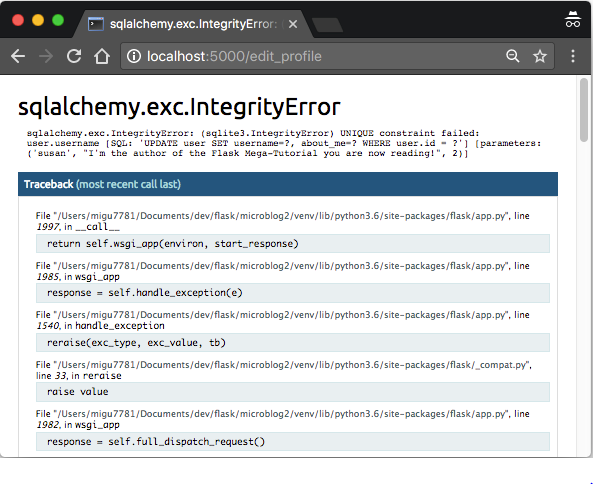
\includegraphics[width=1\textwidth]{figures/5eror.PNG}}
\caption{membuat aplikasi crash.}
\label{eror}
\end{figure}
\ref{eror} dijelaskan bahwa Debugger akan memungkinkan kita meng-expand setiap stack frame dan melihat source code yang terkait. Bisa juga membuka prompt Python di frame manapun dan mengeksekusi perintah Python yang valid, misalnya untuk memeriksa isi dari suatu variabel. Sangat penting untuk tidak mengaktifkan debug mode di production server. Sebagai keamanan tambahan, debugger yang berjalan di browser akan dikunci terlebih dahulu dan meminta nomor PIN yang bisa dilihat saat menjalankan perintah flask run. 


\subsection{Custom Error Pages}
Flask memberikan sebuah mekanisme bagi semua aplikasi untuk memasang halaman error khusus sehingga para user tidak perlu melihat halaman awal yang biasa-biasa saja. Untuk contoh, buat suatu halaman error untuk kode HTTP 404 dan 500, dua kesalahan yang paling sering terjadi pada aplikasi. Membuat halaman untuk halaman error lain tidak berbeda.

Untuk membuat custom error handler, dekorator @errorhandler akan dipakai. Disini akan menulis error handler di file app/errors.py.
app/errors.py: Custom error handlers berikut contohnya :
\begin{verbatim}
from flask import render_template
from app import app, db

@app.errorhandler(404)
def not_found_error(error):
    return render_template('404.html'), 404

@app.errorhandler(500)
def internal_error(error):
    db.session.rollback()
    return render_template('500.html'), 500
 \end{verbatim}
 
Fungsi untuk error handling sangat mirip dengan fungsi view. Untuk kedua jenis error tadi, kita akan menampilkan template khusus. Perhatikan bahwa kedua fungsi tersebut mengirimkan nilai kedua selain template yaitu kode nomor error-nya. Untuk semua fungsi view yang sudah dibuat, tidak perlu mengirimkan kode nomor 200 (untuk menandakan successful response) karena sudah diberikan secara otomatis.
Karena kedua fungsi di atas merupakan fungsi untuk menangani halaman error khusus, maka  perlu memberikan kode status untuk merefleksikan jenis error apa yang akan mereka tangani.

Error handler untuk kode 500 dapat dipanggil setelah sebuah database error, yang salah satu kasusnya terjdi bila ada username yang sama. Untuk memastikan semua percobaan database yang gagal tidak mempengaruhi database yang sudah ada, kita memanggil sesi rollback. Sesi ini akan membersihkan database dari percobaan mengisi data yang sebelumnya gagal (sehingga data yang terubah tidak setengah-setengah).

Berikut ini template untuk halaman error 404:
\begin{verbatim}



    <h1>File Not Found</h1>
    <p><a href="{{ url_for('index') }}">Back</a></p>

 \end{verbatim}
Template meng-extends base.html, sehingga mereka akan memiliki tampilan seperti halaman aplikasi yang normal. 
Agar error handler yang sudah kita tulis terdaftar di Flask, kita perlu mengimpor file app/errors.py sesudah menginisiasi aplikasi
Jika sudah mematikan debug mode dengan FLASK DEBUG 0 di sesi terminal lalu mencoba menganti username sekali lagi, maka kita akan mendapatkan halaman error yang sedikit lebih bersahabat.


\subsection{Mengirim Error Melalui Email}
Masalah lain dengan error handler bawaan Flask adalah tidak ada notifikasi, stack trace untuk setiap error dicetak di terminal, yang artinya output dari proses server harus dimonitor untuk melihat jika terjadi error. Saat aplikasi dijalankan saat melakukan pengembangan hal ini bisa dimaklumi, tapi jika aplikasi sudah di kirim ke server, siapa yang akan memeriksa output yang dikeluarkan? Jadi solusi yang lebih baik diperlukan disini.

Langkah pertama yang mesti dilakukan adalah memberikan detail server email ke file configuration:
Solusi yang akan dilakukan untuk mengatur Flask agar mengirim email setiap terjadi error.
\begin{verbatim}
config.py: Email configuration

class Config(object):
    # ...
    MAIL_SERVER = os.environ.get('MAIL_SERVER')
    MAIL_PORT = int(os.environ.get('MAIL_PORT') or 25)
    MAIL_USE_TLS = os.environ.get('MAIL_USE_TLS') is not None
    MAIL_USERNAME = os.environ.get('MAIL_USERNAME')
    MAIL_PASSWORD = os.environ.get('MAIL_PASSWORD')
    ADMINS = ['your-email@example.com']
    \end{verbatim} 
    
Variabel configuration untuk email diantaranya adalah server, port, penanda untuk mengaktifkan koneksi terenkripsi atau tidak, disertai dengan username dan password. Kelima variabel diambil dari environment variable. Jika server email tidak diatur di environment variable, maka itu akan menjadi pertanda bahwa pengiriman error email perlu dimatikan. Port server email juga perlu dimasukkan di environment variable, tapi jika tidak diatur, port standar nomor 25 akan dipakai. Data username dan password tidak wajib diberikan. Variabel ADMIN adalah daftar email yang akan menerima email error.

Flask menggunakan paket logging dari Python untuk menulis log dan  sudah memiliki kemampuan untuk mengirim log via email. Yang perlu dilakukan untuk mengirimkan pesan log tersebut ke email adalah menambahkan sebuah instance SMTPHandler ke objek Flask logger, yang bernama app.logger  kita hanya akan mengaktifkan email logger jika aplikasi dijalankan tanpa debug mode saat nilai app.debug berisi True juga saat server email ada di file configuration.

Kode-kode di atas akan membuat sebuah instance dari SMTPHandler, mengatur level-nya sehingga hanya membuat laporan error bukan warning, informational atau debugging message, lalu mengirim laporan error tersebut ke objek app.logger dari Flask. Ada dua cara untuk menguji fitur ini. Cara pailng mudah ialah dengan menggunakan server debugging SMTP dari Python. Server ini adalah server email fake , bukannya mengirim, ia akan mencetak email ke console (terminal). 

Untuk menguji kode yang kita buat dengan server ini, atur MAIL SERVER localhost dan MAIL PORT 8025. Jika menggunakan Linux atau Mac OS, perlu menggunakan perintah sudo sehingga perintah tersebut bisa dijalankan. Jika menggunakan Windows, pastikan membuka aplikasi cmd sebagai administrator. Hak akses admin diperlukan dikarenakan port di bawah dari 1024 adalah port yang hanya bisa dijalankan oleh administrator. 

Biarkan server SMTP berjalan lalu kembali ke terminal awal, jalankan perintah export. MAIL SERVER localhost dan MAIL PORT 8025. Pastikan variabel FLASK DEBUG sudah diatur menjadi 0 atau tidak diatur sama sekali, sehingga aplikasi tidak mengirim email dalam debug mode. Jalankan aplikasi dan picu error. SQLAlchemy digunakan untuk melihat terminal yang menjalankan server email fake  yang akan menampilkan sebuah pesan email dengan kode-kode error.
                                                                                                                                          Cara pengujian yang kedua untuk fitur ini adalah dengan menggunakan server email asli. Di bawah ini akan konfigurasi untuk akun server email Gmail sebagai berikut:
\begin{verbatim}
export MAIL_SERVER=smtp.googlemail.com
export MAIL_PORT=587
export MAIL_USE_TLS=1
export MAIL_USERNAME=<your-gmail-username>
export MAIL_PASSWORD=<your-gmail-password>
\end{verbatim}

jika menggunakna Microsoft Windows, selalu gunakan set sebagai ganti export disetiap perintah di atas.

\section{Menyimpan Log Kedalam File}
Menerima error lewat email sangat membantu, tapi terkadang tidak cukup, beberapa kesalahan yang tidak berakhir di exception Python sehingga tidak dianggap sebagai masalah penting, tapi masih berguna untuk tujuan debugging. Oleh karena itu, kita juga akan menyimpan sebuah file log untuk aplikasi ini. Mengaktifkan log file, kita membutuhkan handler lain, RotatingFileHandler perlu untuk ditambahkan ke application logger dengan cara yang tidak jauh berbeda dengan email handler.

app/init.py: Email configuration

\begin{verbatim}
# ...
from logging.handlers import RotatingFileHandler
import os

# ...

if not app.debug:
    # ...

    if not os.path.exists('logs'):
        os.mkdir('logs')
    file_handler = RotatingFileHandler('logs/microblog.log', maxBytes=10240,
                                       backupCount=10)
    file_handler.setFormatter(logging.Formatter(
        '%(asctime)s %(levelname)s: %(message)s [in %(pathname)s:%(lineno)d]'))
    file_handler.setLevel(logging.INFO)
    app.logger.addHandler(file_handler)

    app.logger.setLevel(logging.INFO)
    app.logger.info('Microblog startup')
\end{verbatim}

Disini penulis membuat file log bernama microblog.lo di dalam direktori/folder logs, yang akan dibuatkan jika belum ada. Kelas RotatingFileHandler sangat berguna karena merotasi file log, memastikan bahwa file log tidak berukuran terlalu besar saat aplikasi sudah berjalan cukup lama. Dalam kasus ini, penulis membatasi ukurannya menjadi 10KB, dan penulis menyimpan 10 file log terakhir untuk serep. 

Kelas logging.Formatter akan memberikan sebuah formatting dalam penulisan pesan log. Karena pesan-pesan ini akan disimpan ke dalam sebuah file, maka kita akan menyimpan informasi sebanyak-banyaknya. Oleh karena itu, kita akan menggunakan format yang memiliki timestamp, logging level, isi pesan error dan nama file serta nomor baris yang menyebabkan sesuatu terjadi.

Agar proses logging bisa menangkap lebih banyak pesan, dapat dilakukan dengan cara menurunkan logging level ke kategori INFO yang biasanya digunakan untuk application logger maupun file logger handler. Jika tidak familiar dengan kategori loggin, ada DEBUG, INFO, WARNING, ERROR, dan CRITICAL.  Ketika aplikasi ini berjalan di server produksi, entri log akan memberi tahu server direstart.


\section{Cara Memperbaiki Bug Duplikasi Username}
Untuk memperbaiki bug username yang sebelumnya telah ditemukan, sebelumnya, RegistrationForm sudah mengimplementasi validasi untuk username, tapi validasi yang dilakukan di form edit sedit berbeda. Saat registrasi, pastikan bahwa username yang dimasukkan belum ada di database. Pada halaman edit profil kita juga harus melakukan pemeriksaan yang sama.


\chapter[Postman dan Swagger]
{Postman dan Swagger}

\documentclass[12pt,a4paper]{article}
\usepackage[left=3.00cm, right=2.00cm, bottom=2.00cm, top=3.00cm]{geometry}
\usepackage{graphics}
\begin{document}
\title{Postman dan Swagger}
\maketitle
\begin{enumerate}
\item Fransiscus Ivan Martongam      1164039 \\
\item Lalita Chandiany Adiputri      1164043\\
\item Eko Cahyono Putro              1164035\\
\item Lidwina Triniska Gulo          1164044\\
\item Sulpadianti Bunyamin           1164096\\
\end{enumerate}

\section{Pengertian Postman}
Postman merupakan sebuah software yang memuat fungsi lengkap pengembangan sistem dalam mengirimkan dan menerima respon server. Software ini mendukung pengembangan sistem REST API dengan mengklasifikasi request berdasarkan request method, URL dan parameter-parameter request. Postman juga adalah sebuah aplikasi (berupa plugin) untuk browser chrome, fungsinya adalah sebagai REST Client atau istilahnya adalah aplikasi yang digunakan untuk melakukan uji coba REST API yang telah kita buat.

\section{Fungsi dari postman}
Menurut Arianto M A, DKK(2016), Sebuah aplikasi yang digunakan untuk melakukan uji coba REST API yang telah kita buat. Fungsi Postman adalah untuk pengecekan web service. Postman dapat menampilkan hasil dari HTTP request yang kompleks sekalipun dengan cepat. Postman muncul sebagai add-on dari chrome namun sekarang sudah menjadi aplikasi native. Postman memudahkan untuk menguji, mengembangkan dan API (Application Programmin Interface) dokumen dengan memungkinkan pengguna untuk dengan cepat mengumpulkan baik permintaan HTTP sederhana dan kompleks

\section{cara instal postman}
Postman for Chrome (aplikasi Postman sebelumnya merupakan ekstensi Chrome App atau aplikasi yang menginduk pada Chrome).
Cara menginstal Postman untuk menginstal Postman versi native pada sistem operasi Ubuntu/Debian yaitu 
Buka terminal lalu unduh atau donwload paket instalasi Postman dengan mengunakan perintah wge,
kemudia Ekstrak file instalasi Postman tersebut ke direktori /optsudo tar -xzf postman.tar.gz -C /opt.
setelah itu dapat menghapus file instalasinya (opsional)dengan cara rm postman.tar.gz


\section{membuat shortcut Postman}
Berikut tata cara untuk membuat shortcut pada start menu postman.  Ketik perintah - perintah berikut dibawah ini:
cat > ~/.local/share/applications/postman.desktop <<EOL
[Desktop Entry]
Encoding=UTF-8
Name=Postman
Exec=postman
Icon=/opt/Postman/resources/app/assets/icon.png
Terminal=false
Type=Application
Categories=Development;
EOL

Sekarang untuk membuka aplikasi yang ada pada Postman , cukup hanya dengan melakukan klik pada shortcut pada start - menu. 

\section{Cara Penggunaan Postman}
Berikut cara penggunaan Postman : Buat sebuah file baru pada direktori root webserver dengan nama: contoh-api-sederhana.php .Kemudian ketikan kode PHP berikut ke dalam file contoh-api-sederhana.php. Berikut kode untuk membuat file:

\begin{figure}[ht]
\centerline{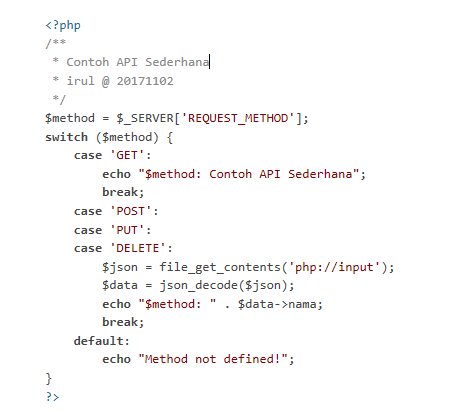
\includegraphics[width=1\textwidth]{figures/3contohapi.PNG}}

\caption{Contoh Api Sederhana} 
\label{api}
\end{figure}

pada gambar \ref{api} menjelaskan tentang contoh api.

Pada file contoh-api-sederhana.php, dapat didefinisikan satu buah API dengan empat Http Request Method yang berbeda. Berikut daftar method dan alamat url yang nanti akan kita uji menggunakan Postman:
•	GET => /contoh-api-sederhana.php
•	POST => /contoh-api-sederhana.php
•	PUT => /contoh-api-sederhana.php
•	DELETE => /contoh-api-sederhana.php
Kita dapat menguji salah satu API di atas menggunakan browser, salah satunya, menggunakan method GET, browser akan mengirimkan data ke server menggunakan method GET.

\section{Implementasi Postman}
Implementasi tidak hanya aktivitas, melainkan suatu kegiatan yang terencana untuk mencapai
tujuan kegiatan. Tahap implementasi pada penelitian ini tidak dilakukan hanya dalam satu proses,
Tetapi dilakukan dalam beberapa sub proses yaitu membangun lingkungan pengembangan sistem, 
mendesain struktur table, function dan stored procedure pada database, mengembangkan sistem back-end (coding) 
dan menyesuaikan dengan database, dan mendesain struktur rewrite pada web server. 

\section{Pengujian}
Untuk memastikan bahwa sistem berjalan sesuai dengan rencana pengembangan sistem dan proses bisnis yang difasilitasi, diperlukan sebuah skenario pengujian sistem. Pada penelitian ini, pengujian akan dilakukan dengan menggunakan software Postman dan dibagi menjadi tiga skenario pengujian, yaitu: Pengujian otentikasi token untuk memastikan prinsip REST terpenuhi, pengujian dengan metode equivalent partitioning untuk memastikan nilai-nilai masukan sesuai dengan rencana pengembangan sistem, pengujian fungsional untuk memastikan setiap titik akses API.

\subsection{Pengujian otentikasi token}
Pengujian  otentikasi token dilakukan pada load-balanced server dengan jumlah back-end server sebanyak tiga virtual server yang diklasifikasi berdasarkan port jaringan. Pengujian  metode equivalent partitioning akan mengelompokkan nilai masukan ke dalam kelas- kelas kemudian diuji dalam kasus-kasus tertentu. Pengujian fungsional dilakukan secara langsung setiap titik akses sistem API yang telah dibuat. 

\subsection {Pengujian dengan metode equivalent partitioning}
Pengujian dengan menggunakan metode equivalent partitioning ini untuk memastikan nilai-nilai masukan sesuai dengan rencana pengembangan sistem. Pengujian ini akan mengelompokkan nilai masukan ke dalam kelaskelas batasan nilai untuk kemudian diuji dalam kasus-kasus tertentu. Rencana pengujian metode ini meliputi validasi path, validasi request method, validasi token, kesesuaian tipe data dan validasi nilai.


\end{document}



\chapter[Hello World di Flask]
{Hello World di Flask}
%Resume Hello word di Flask

%Kelompok 2 D4 TI / 2B

%Alwan Suryansah				1164033 
%Dinda Ayu Pratiwi				1164034
%Kurnia Sandi					1164042
%Teduh Sanubari					1164054
%Wildan Khaustara Wijaksana		1164058

\documentclass[12pt]{article}
\usepackage[pdftex]{graphicx}
\usepackage{epstopdf}
\usepackage{graphics}


\begin{document}
\section{Apa itu Flask?}
\subsection{menurut Pennanen, Jussi and others}
Flink adalah kerangka kerja pada perangkat lunak yang dikembangkan bertujuan untuk pelaksanaan pada aplikasi Web dalam bahasa pemrograman Python. Fcalculator pembangunan dimulai tahun 2010 oleh pengembang utama yaitu Armin Ronacher. Mencakup kerangka, antara hal-hal lain, Jinja2-templateengine, dan server pengembangan yang memfasilitasi pengembangan. Flask berlisensi di bawah lisensi BSD\cite{pennanen2018sovellus}.

\subsection{Menurut Nandana Adya Samudera}
Flask adalah sebuah aplikasi microframework untuk bahasa, Python yang dibuat dengan toolkit Werkzeug dan template Jinja2. Flask dibuat oleh Armin Ronacher. Pertama kali dirilis pada April 2010. Bila dibandingkan dengan Django, Flask jauh lebih ringan dan cepat karena Flask dibuat dengan ide menyederhanakan inti frameworknya seminimal mungkin, dengan tagline “web development, one drop at a time”, oleh karena itu Flask disebut microframework. Flask dapat membantu kita membuat situs dengan cepat meskipun dengan library yang sederhana. Contoh aplikasi yang menggunakan framework Flask adalah Pinterest, dan LinkdIn. Flask saat ini berada pada lisensi 0.10.1 dan dilisensikan dengan lisensi BSD.

Aplikasi yang dibuat dengan framework Flask disimpan dalam satu berkas “.py”. Flask adalah framework yang dikolaborasikan dengan bahasa python yang sederhana namun dapat diperluas dengan beragam pustaka tambahan yang disesuaikan dengan kebutuhan penggunanya. Meskipun Flask belum menyampai versi 1.0 namun dokumentasi yang dmilikinya sangat lengkap yang dapat kita gunakan untuk membuat aplikasi atau situs dengan cepat\cite{samudera2015perancangan}.

\subsection{Menurut Gunawan, Andre and Palit, Henry Novianus and Handojo, Andreas}
Flask merupakan microframework yang dibangun dengan menggunakan bahasa pemrograman Python. Flask digunakan untuk me-develop sebuah aplikasi web. Flask merupakan microframework yang artinya flask membuat sebuah pengerjaan aplikasi web menjadi mudah dan simple karena dapat menjalankan sebuah web hanya dengan menggunakan 1 file Python. Flask membuat susunan kerja yang ringan, dan mudah tetapi juga dapat dikembangkan dengan mudah\cite{gunawan2018aplikasi}.

\subsection{Menurut jurnal Ash-shidiq, Usamah and Rumani, M and Saputra, Randy Erfa}
Flask adalah sebuah microframework yang berbasis python dan dipelopori oleh Armin Ronacher. Bila dibandingkan dengan Django, Flask jauh lebih ringan dan cepat karena Flask dibuat dengan ide menyederhanakan inti framework nya seminimal mungkin dan seefesien mungkin. Flask dapat membantu dalam membuat situs dengan sangat cepat dan mudah meskipun dengan librari yang lumayan sederhana\cite{ash2017perancangan}.

\subsection{Flask menurut Reza, Robby and Jati, Agung Nugroho and Ahmad, Umar Ali}
Flask merupakan sebuah micro framework yang berbasis kan baha pemrograman python kemudian di pelopori oleh Armin Ronacher . Flask apabila  di bandingkan dengan Django, Flask akan lebih jauh ringan  cepat dan mudah  karena  Flask  dibuat   dengan  ide  untuk menyederhanakan  inti  framework-nya  sebaik  mungkin. Dengan sebuah tag line “web development, one drop at a time”, Flask dapat membantu kita membuat situs dengan sangat cepat meskipun dengan library yang sederhana\cite{reza2016perancangan}.

\subsection{menurut Grinberg, Miguel}
Ada sekali Bahasa pemrograman yang digunakan sebagai framework contohnya Bahasa pemrograman python, diantaranya Django, Flask, Pyramid, Tornado, Bottle, Diesel, Pecan, Falcon dan yang lainnya.Pada tulisan ini, penulis ingin membahas tentang penggunaan Flask sebagai framework untuk menunjang cloud server yang dibuat. Flask merupakan microframework berbasis Bahasa pemrograman python yang dipelopori oleh Armin Ronacher. Bila dibandingkan dengan Django, Flask ini memiliki keunggulan jauh lebih ringan dan lebih cepat \cite{grinberg2018flask}.

\subsection{Menurut Alauddin, Muhammad Fikri}
Flask adalah sebuah microframework untuk Python berbasis Werkzeug, Jinja 2 dan niat baik.Flask berfungsi sebagai pengganti PHP POST dan GET yang dimana pengendali pertukaran data dari HTML ke database. Flask juga menggantikan fungsi Apache sebagai webserver dimana flask berjalan di http://localhost:5000/ \cite{alauddin2017implementasi}.

\subsection{Flask Adalah Implementasi dari web API menurut Jurnal ULTIMA}
Flask API merupakan implementasi dari web sebuah API yang dapat dijelajahi menggunakan kerangka yang sudah disediakan oleh Django REST. Django REST merupakan web framework dengan sumber terbuka yang berbasiskan Python, Aplikasi web yang dibuat menggunakan Flask disimpan dalam satu berkas .py. Flask merupakan web framework yang sederhana namun dapat diperluas dengan beragam pustaka tambahan yang sesuai dengan kebutuhan penggunanya. Flask API menyimpan perintah-perintah dari gphoto library dan piggyphoto library\cite{computingaplikasi}. 

\section{Aturan-Aturan Flask}

 
 
\section{Membuat "Hello World" di Flask}
\subsection{Membuat "Hello World" dengan Flask menurut Lokhande, PS and Aslam, Fankar and Hawa, Nabeel and Munir, Jumal and Gulamgaus, Murade}
Program Hello World di Flask adalah contoh dasar Flask di mana kita mengimpor kelas Flask menggunakan fungsi impor, kemudian kita mendefinisikan fungsi hello world dan kemudian mengembalikan 'Hello World!' \cite{lokhande2015efficient}.
\begin{verbatim}
from flask import Flask
app = Flask(__name__)
@app.route('/')
def hello_world():
return 'Hello World!'
if __name__ == '__main__':
app.run()
\end{verbatim}

\subsection{Membuat "Hello World" dengan Flask menurut Maia, Italo}
dibawah ini merupakan cara membuat hello wold pada bahasa pemrograman pyton yaitu menggunakan flask ,dimana kita akan mengimport dan membuatnya menjadi "hello world" perhatikan code dibawah ini ;
\cite{maia2015building}.
\begin{verbatim}
# coding:utf-8
from flask import flask 
app = Flask(__name__)

@app.route('/')
def hello():
	return "Hello World!"
	
if __name__ == '__main__':
app.run()
\end{verbatim}

\subsection{Membuat "Hello World" dengan Flask menurut Aggarwal, Shalabh }
Flask bertujuan menjaga inti dari kerangka kecil tetapi sangat extensible. Ini membuat aplikasi atau ekstensi menulis sangat mudah dan fleksibel dan memberi pengembang kekuatan untuk memilih konfigurasi yang mereka inginkan untuk aplikasi mereka, tanpa memaksakan pembatasan pada pilihan basis data, mesin templating, dan seterusnya\cite{aggarwal2014flask}.

Menyiapkan aplikasi Hello World sederhana :
\begin{verbatim}
from flask import Flask
app = Flask(__name__)
@app.route('/')
def hello_world():
return 'Hello to the World of Flask!'
if __name__ == '__main__':
app.run()
\end{verbatim}

\subsection{Membuat Hello World dengan Flask menurut Grinberg, Miguel}
Versi kedua dari aplikasi ini yaitu menambahkan sebuah rute yang dinamis. Ketika Anda mengunjungi URL dinamis di browser Anda, Anda akan disajikan dengan ucapan pribadi yang menyertakan nama yang diberikan di URL. Contoh aplikasi Flask dengan rute dinamis.
\begin{verbatim}
From Flask import Flask
app = Flask(__name__)
@app.route(‘/’)
def index():
	return ‘<h1>Hello World !</h1>’
@app.route(‘/user/<name>’)
def user(name):
	return  ‘<h1> Hello, {}!</h1>’.format(name)

\end{verbatim}
Jika Anda telah mengkloning repositori git aplikasi di GitHub, Anda sekarang dapat menjalankan git untuk memeriksa versi aplikasi ini\cite{grinberg2018flask}.

\subsection{Hello World Dengan Flask Oleh Alessandro Zini}

Bahasa yang digunakan untuk implementasi logika sisi server dan Python 2.7: perlu untuk dilarifikasi bahwa, terlepas dari pilihan tersebut bahwa akan diambil beberapa pustaka yang digunakan tidak memperpanjang dukungan ke versi 3 dari Python.

Untuk memahami fungsi kerangka kerja Flask dan proyek Contoh klasik ilmu komputer diusulkan: Hello World.

\begin{verbatim}
from flask import Flask
app = Flask(__name__)
@app.route("/", methods=["GET"])
def hello_world():
return "Hello, World!"
\end{verbatim}

Hasil dari kode ini dan tampilan halaman web yang berisi string "Hello, World!". Yang pertama diimpor sebagai operasi pertama Kelas flask, instantiate suatu objek. Parameter yang ditentukan dan variabel khusus: "nama".  Variabel ini digunakan di lingkungan Python, dan masih banyak lagi yang lebih spesifik dari Flask, untuk mengidentifikasi apakah modul saat ini telah tersedia di aplikasi utama saya, atau bisa diimpor dari modul eksternal; di kasus pertama, kita akan memiliki nilai utama, keduanya akan berisi nama modul eksternal dari mana modul yang saat ini diimpor. Mekanisme ini diakali dan digunakan oleh Flask untuk mengatur parameter pencarian dengan benar\cite{ziniqr}.

\subsection{Hello World Flask by Django, Flask}
Routes merupakan sebuah kumpulan dari URL kemudian di implementasi oleh aplikasi. Dalam FLask, handler merupakan route aplikasi yang ditulis sebagai fungsi dari Python yang disebut dengan view function. View function akan memetakan satu atau lebih URL sehingga Flask akan tahu apa yang harus ia lakukan setiap kali klien memanggil sebuah URL. Berikut ini merupakan contoh Flask Route\cite{djangoweb}.
\begin{verbatim}
import flask

app = flask.Flask(__name__)

@app.route('/')

def hello():

return 'Hello’

app.run()

\end{verbatim}

\subsection{Hello World di Flask menurut Buku Learning Flask Framework}
Satu hal yang sangat berguna untuk dilakukan dengan Flask adalah membuat UI dengan baris perintah sehingga, ketika orang lain menggunakan perangkat lunak Anda, mereka dapat dengan mudah menggunakan metode yang Anda berikan, seperti mengatur database, membuat pengguna administratif, atau memperbarui Kunci rahasia CSRF.

Satu area di mana kita sudah memiliki skrip yang menyerupai ini dan salah satu yang dapat digunakan dengan cara ini adalah Script ... di Bab 2, Relational Databases dengan SQLAlchemy. Untuk melakukan ini, ada lagi, ekstensi Flask. Cukup jalankan perintah berikut:

\begin{verbatim}
pip instal Flask-Script
\end{verbatim}



\section{Error yang Muncul serta Solusinya}



\section{Implementasi dengan menggunakan Flask}
Implementasi web service menggunakan flask web framework, library pandas untuk membaca file csv dan membentuk fitur matrix X dan vektor target y. Penggunan library scikit learn agar dapat menggunakan modul naive bayes, serta untuk melakukan pembagian data training dan testing dengan fungsi train test split. Modul terakhir yang digunakan adalah pickle untuk menyimpan classifier yang telah dibuat ke dalam disk, agar tidak melakukan training berulang-ulang untuk setiap request yang dikirim.

Listing program 1 berfungsi untuk membuat naive bayes classifier, kemudian menyimpannya dengan nama nbp imadiebetspkl agar dapat dipanggil oleh web service. Listing program 2 menampilkan kode pembuatan web service yang diimplementasikan pada fungsi predict, sedangkan Listing program 3 menampilkan contoh kode aplikasi dalam bahasa python yang melakukan request ke web service dengan mengirimkan parameter 'pregn':6,'gluc':148,
'bp':72,'sk':35,'ins':0,
'bmi':33.6,'ped':0.627,'age':50, dimana akan menghasilkan variabel output dengan nilai {'results': [1]} yang berarti positif diabetes \cite{setyawan2017implementasi}.

\begin{verbatim}
Listing program 1. Pembuatan naive bayes classifier
url = 'pima-indians-diabetes.csv'
col_names = ['pregnant', 'glucose', 'bp', 'skin',
'insulin', 'bmi', 'pedigree', 'age', 'label']
pima = pd.read_csv(url, header=None, names=col_names)
feature_cols = ['pregnant', 'glucose', 'bp', 'skin',
'insulin', 'bmi', 'pedigree', 'age']
X = pima[feature_cols]
y = pima.label
X_train, X_test, y_train, y_test =
train_test_split(X, y, stratify=y, test_size=0.25, random_state = 0)
nb = GaussianNB()
nb.fit(X_train, y_train)
pickle.dump(nb, open("nb_pimadiabtes.pkl","wb"))

Listing program 2. Implementasi web service dengan flask
import numpy as np
from flask import Flask, request, abort, jsonify
import pickle
nbclassifier = pickle.load(open("nb_pimadiabtes.pkl","rb"))
app = Flask(__name__)
@app.route('/api', methods=['POST'])
def predict():
data = request.get_json(force = True)
predict_request = [data['pregn'],data['gluc'],data['bp']
data['sk'],data['ins'],data['bmi'],data['ped'],data['age']]
predict_request = np.array(predict_request)
y_result = nbclassifier.predict(predict_request)
output = [int(y_result[0])]
return jsonify(results=output)
if __name__ == '__main__':
app.run(debug = True)

Listing program 3. Contoh kode yang mengakses web service
import json
import requests
url = "http://127.0.0.1:5000/api"

Listing program 3. Lanjutan
data= json.dumps({'pregn':6,'gluc':148,'bp':72,'sk':35,
'ins':0,'bmi':33.6,
'ped':0.627,'age':50})
r = requests.post(url, data)
output = r.json()
\end{verbatim}






\section{Kesimpulan}
Dari berbagai pengertian mengenai bahasa pemograman flask kita dapat simpulkan bahwa bahasa pemograman flask merupakan bahasa pemrograman open source yang banyak digunakan untuk menangani beberapa jenis masalah dalam pemrograman salah satunya membuat suatu framework. flask banyak digunakan untuk meningkatkan kualitas perangkat lunak, produktivitas pengembang, portabilitas program, dan integrasi komponen.

kata lain Flask adalah framework aplikasi web mikro yang ditulis dalam bahasa Python dan berbasiskan toolkit Wekzeug dan template engine Jinja2 dan berlisensi BSD. Pada tahun 2015, versi paling stabil Flask adalah versi 0.10.1. Contoh aplikasi yang menggunakan framework Flask adalah Pinterest, LinkedIn, dan tentu saja halaman web Flask itu sendiri.

Flask dikatakan framework mikro dikarenakan Flask tidak menganggap atau mengharuskan pengembang menggunakan alat atau pustaka tertentu. Flask tidak memiliki lapisan abstrak basis data, validasi form, dan komponen-komponen lainnya yang sudah dimiliki oleh pustaka-pustaka pihak ketiga sebelumnya. Walaupun begitu, Flask mendukung ekstensi yang dapat menambah fitur-fitur seperti layaknya mereka diimplementasikan di dalam Flask itu sendiri. Terdapat ekstensi untuk object-relational mappers, validasi form, upload handlint, dan berbagai teknologi otentikasi terbuka serta peralatan yang berhubungan dengan framework secara umum\cite{solihin2016implementasi}. 

maka dari dibuatnya resume ini kita dapat mengetahui: 
	
\begin{enumerate}
\item mengetahui apa itu flask.
\item wawasan lebih luas tentang flask
\item mengetahui bagaimana cara pembuatan "hello world di flask"
\item mengetahui cara memecahkan masalah pada suatu error code di flask.
\end{enumerate}	


Cukup sekian yang dapat kami sampaikan semoga resume ini dapat bermanfaat bagi pembaca maupun penulis , mohon maaf jika masih banyak kesalahan dalam hal penulisan maupun dalam hal penyampaian materi flask ini, kami harapkan kritik dan saran supaya dapat membuat resume menjadi lebh baik lagi untuk kedepanya kami ucapkan trimakasih banyak  .
\end{document}







\chapter[GET]
{Parameter GET}
%Resume GET (parameter GET, cara penggunaan dan kode) Kelompok 3 D4TI2B
%\begin{enumerate}
%\Fikri aldi nugraha                  1164038
%\Nur Arkhamia Batubara               1164049 
%\Miftahul Hasanah                    1164046 
%\Si Made Angga Dwitya P              1164053 
%\Widary Anggraini Mindo V Siahaan    1164057
%\end{enumerate}

\section{Pengenalan Method GET Pada HTTP}
HTTP mendefinisikan seperangkat metode permintaan untuk menunjukkan tindakan yang diinginkan yang akan dilakukan untuk sumber daya tertentu.
Meskipun mereka juga bisa menjadi kata benda, metode permintaan ini kadang-kadang disebut sebagai verba HTTP. Masing-masing menerapkan semantik yang berbeda, namun beberapa fitur umum digunakan bersama oleh mereka: mis. Metode permintaan dapat berupa safe, idempotent, atau cacheable. 
Salahsatu metode permintaan yang digunakan dalam Http adalah GET, dimana GET ini digunakan untuk meminta representasi sumber atau menampilkan data/nilai pada url yang nantinya akan ditampung oleh action.


\chapter[Json dan YAML]
{JSON dan YAML}
\documentclass[a4paper]{article}
\usepackage{graphicx}
\begin{document}
\section{JSON}
\subsection{Definisi JSON}
JSON atau JavaScript Object Notation adalah salah satu bentuk format yang ringkas untuk melakukan pertukaran sebuah data di dalam computer. JSON sendiri berbasis teks dan mudah untuk dibaca oleh manusia serta dapat digunakan untuk representasi struktur data sederhana JSON juga dapat digunakan untuk proses transmisi data terstruktur melalui media koneksi jaringan yang disebut Serialisasi.
\subsection{Definisi JSON}
JSON  adalah  bagian  dari  sebuah bahasa  pemrograman  JavaScript  JSON juga merupakan format teks yang sepenuhnya independen tetapi menggunakan konvensi yang  familiar  dengan  bahasa  pemrograman  dari  parent-C,  termasuk  bahasa C,  Java,  Java Script,  Perl, Python,  dan lain sebagainya.  Kelebihan  inilah  yang  membuat  JSON  menjadi  sebuah  bahasa yang disebut  data-interchange yang ideal.
\subsection{Struktur pada JSON}
JSON memiliki 2 struktur,yaitu:
1.	Kumpulan pasangan nama/nilai.
Dalam beberapa Bahasa pemrograman, ini biasanya sering disebut seperti objek, rekaman, struktur, kamus, tabel hash, daftar berkunci atau array assosiatif.
2.	Daftar nilai terurutkan.
Dalam kebanyakan Bahasa pemrograman, ini biasanya sering disebut seperti array, vektor, daftar, atau urutan.
Struktur data tersebut sering kali disebut sebagai struktur data universal. Semua bahasa pemrograman modern mendukung struktur data tersebut dalam bentuk yang sama maupun berbeda.
\subsection{Pengertian Lain Dari JSON}
JSON atau biasa dilafalkan dengan “Jason” merupakan singkatan dari JavaScript Object Notation adalah suatu format ringkas pertukaran data computer. Format Json berbasis teks dan mudah dibaca-manusia serta digunakan untuk merepresentasikan struktur data sederhana dan larik asosiatif. JSON juga seringkali digunakan untuk transmisi datayang  terstruktur melalui suatu koneksi jaringan pada suatu proses yang disebut serialisasi.

\section{YAML}
\subsection{Definisi YAML}
YAML atau YAML Ain't Markup Language adalah sebuah standar yang sudah umum untuk digunakan proses Serialisasi data dalam semua Bahasa pemrograman. YAML dapat memberikan representasi data dengan bentuk yang lebih sederhana. Salah satu bentuk penyederhanaan nya adalah dengan menghilangkan tanda {} dan tanda []. YAML sendiri juga memiliki fitur yang tidak dimiliki oleh JSON.
\begin{figure}[ht]
\centerline{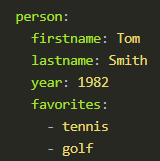
\includegraphics[scale=1]{../figures/5SC.png} }

\caption{Contoh Source Code} 
\label{Sc}
\end{figure}

Pada gambar \ref{Sc} dijelaskan tentang Contoh Source Code.

\subsection{Definisi Lain dari YAML}
YAML merupakan format serial data yang dapat dibaca oleh manusia yang mengambil beberapa bahas apemrograman seperti XML, C, Python, serta format email seperti yang recantum dalam RFC 2822. Pengusul YAML adalah Clark Evans pada tahun2001 silam. Clark merancang format ini bersama dengan Ingy döt Net dan Oren Ben-Kiki. YAML pula tersedia dalam beberapa Bahasa dan script pemrograman.
\subsection{YAML}
YAML mengintegrasikan dan membangun berdasarkan konsep yang dijelaskan oleh bahasa C, Java, Perl, Python, Ruby, RFC0822 (MAIL), RFC1866 (HTML),RFC2045 (MIME), RFC2396 (URI), XML, SAX, SOAP, dan JSON.
Sintaks YAML motivated oleh Internet Mail (RFC0822) dan tetap sebagian kompatibel dengan standar itu. selanjutnya, meminjam dari MIME (RFC2045), produksi tingkat atas YAML adalah aliran dokumen independen, ideal untuk pesan berbasissistem pemrosesan terdistribusi.
\subsection{Definisi YAML}
Pada saat awal-awal perkembangan, YAML diartikan dari banyak orang adalah sebuah singkatan yaitu "Yet Another Markup Language". Namun seiring berkembangnya zaman, untuk memberitahu tujuannya lebih jauh yang terfokus pada data dan bukan markah dokumen, akhirnya singkatan YAML diubah menjadi "YAML Ain't a Markup Language." YAML tersedia untuk beberapa Bahasa dan skrip pemrograman.
\subsection{YAML}
Dari pembahasan di atas, yang telah membahas tentang JSON atau JavaScript Object Notation dan YAML atau YAML Aint Markup Language. Berdasarkan pembahasan di atas dapat di temukan perbedaan antara keduanya. Berikut adalah beberapa perbedaan yang dapat kami kemukakan :
Berikut adalah tabel \ref{table:perbedaan} perbedaan JSON dan YAML.
\begin{table}[h]
\caption{Perbedaan JSON dan YAML}

\centering
\begin{tabular}{ccc}
\hline
&JSON&YAML\\
\hline
Kegunaan&Cocok untuk Format Serialisasi&Cocok untuk konfigurasi\\
\hline
Fitur&tidak memiliki komentar, aliasing&memiliki komentar, aliasing \\
&dan anchoring, dan  mergering& dan anchoring, dan  mergering\\
\hline
\end{tabular}
\label{table:perbedaan}
\end{table}

\end{document}

\chapter[Upload File di Flask]
{Upload File di Flask}
\documentclass[12pt,a4paper]{article}
\usepackage[left=3.00cm, right=2.00cm, bottom=2.00cm, top=3.00cm]{geometry}
\linespread{1.5}
\begin{document}
\title{definisi Dekorator, Contoh Kode dan Fungsi}
\maketitle

\begin{itemize}

\item
NAMA KELOMPOK 4\\
Ajis Trigunawan			1164031\\
Alimu Dzul Ikroom		1164032\\
Muhammad Hanafi			1164092\\
Riki Karnovi			1164052\\
Yoga Sakti Hadi P		1164059\\

\end{itemize}

\section{Cara Upload File di Flask}

\subsection{Pengantar Flask}

Flask framework didasarkan pada Werkzeug, dan Jinja 2, dan intensitas yang baik. Kerangka ini tidak memiliki dependensi terpisah dari
Perpustakaan Standar Python. Labu tidak termasuk komponen yang membutuhkan pihak ketiga dukungan seperti memvalidasi formulir atau menyediakan sarana komunikasi antara aplikasi dan database. Namun, fitur tersebut dapat ditambahkan menggunakan ekstensi. Layanan yang ditawarkan oleh kerangka ini termasuk server HTTP built-in, dukungan untuk pengujian unit, dan Layanan web RESTful. Aplikasi dibangun menggunakan ini kerangka kerja adalah minitwit, flaskr, flask.pocoo.org dll.

\subsection{Cara Mengunggah File}


Di sini Kita bisa mengupload file atau gambar dalam framework flask seperti halnya framework lainya. Akan tetapi Flask membuat kita bisa dengan mudah mengupload gambar atau file hingga menampilkannya sesuai keinginan kita. Kita disini akan menggunakan werkzeug untuk mengupload file di flask. Werkzeug yang merupakan modul bawaan flask dapat menangani itu semua.
File yang kita upload akan kita simpan ke dalam server dan bukan database karena database didesain untuk tidak digunakan sebagai penyimpanan file sebab jika database penuh dengan file maka itu hanya akan menghancurkan database dan menurunkan performa database anda. Namun kita bisa menyimpan nama file kedalam database untuk bisa mengquery file yang tersimpan didalam server.

Dibawah ini merupakan langkah-langkah yang harus anda lakukan untuk mengupload file di flask.

Kita harus membuat database terlebih dahulu dan seperti biasa database yang kita gunakan adalah sqlalchemy. Database bisa terlihat sebagai berikut
\begin{verbatim}
from app import app, db
class User(db.Model):
    id = db.Column(db.Integer, primary_key=True)
    username = db.Column(db.String(500))
    name = db.Column(db.String(64))
\end{verbatim}

Penanganan upload file dalam Flask ada beberapa hal yang harus disiakpak. Diperlukan formulir HTML dengan atribut enctype yang disetel ke ‘multipart / form-data’, mengeposkan file ke URL. Penangan URL mengambil file dari request.files [] objek dan menyimpannya ke lokasi yang diinginkan.
Setiap file yang diunggah pertama-tama disimpan di lokasi sementara di server, sebelum benar-benar disimpan ke lokasi terakhirnya. Nama file tujuan dapat dikodekan atau dapat diperoleh dari properti nama file dari objek request.files [file]. Namun, disarankan untuk mendapatkan versi aman menggunakan fungsi secure filename ().

Anda dapat menentukan jalur folder upload default dan ukuran maksimum file yang diunggah dalam pengaturan konfigurasi objek Flask.
Menentukan jalur untuk folder unggah
\begin{verbatim}
app.config [‘UPLOAD_FOLDER’] 
\end{verbatim}
Menentukan ukuran maksimum file yo diunggah - dalam byte
\begin{verbatim}
app.config [‘MAX_CONTENT_PATH’] 
\end{verbatim}
Kode berikut memiliki aturan ‘/ unggah’ yang menampilkan ‘upload.html’ dari folder template, dan aturan URL ‘/ upload-file’ yang memanggil uploader () fungsi penanganan proses upload.

Kita dapat memproses file yang akan diupload dengan Flask dengan mudah. Sebelumnya pastikan jangan lupa untuk mengatur atribut enctype = "multipart/form-data" pada form HTML kita, jika tidak browser tidak akan mengirimkan file Anda sama sekali. File yang diunggah disimpan di memori atau di lokasi sementara di sistem file kita. Berikut ini contoh sederhana yang menunjukkan cara kerjanya:

‘Upload.html’ memiliki tombol pemilih file dan tombol kirim..
\begin{verbatim}
<html>
   <body>
   
      <form action = "http://localhost:5000/uploader" method = "POST" 
         enctype = "multipart/form-data">
         <input type = "file" name = "file" />
         <input type = "submit"/>
      </form>
      
   </body>
</html
\end{verbatim}
untuk routenya kita membuat parameter /upload dan menggunakan method get dan post seperti berikut ini:

\begin{verbatim}
from flask import request

@app.route('/upload', methods=['GET', 'POST'])
def upload_file():
    if request.method == 'POST':
        f = request.files['the_file']
        f.save('/var/www/uploads/uploaded_file.txt')
    ...
\end{verbatim}
Dan jika Anda ingin tahu bagaimana file itu diberi nama pada klien sebelum diunggah ke aplikasi Anda, Anda dapat mengakses atribut filename.
Klik Kirim setelah memilih file. Metode entri Formulir memanggil URL '/ uploadfile'. Pengunggah fungsi yang mendasarinya () melakukan operasi penyimpanan.

Penanganan upload file dalam Flask sangat mudah. Diperlukan formulir HTML dengan atribut enctype yang disetel ke ‘multipart / form-data’, mengeposkan file ke URL. Penangan URL menjemput file dari request.files [] objek dan menyimpannya ke lokasi yang diinginkan.
	Setiap file yang diunggah pertama-tama disimpan di lokasi sementara di server, sebelum benar-benar disimpan ke lokasi terakhirnya. Nama file tujuan dapat dikodekan atau dapat diperoleh dari properti nama file dari objek request.files [file]. Namun, disarankan untuk mendapatkan versi aman menggunakan fungsi secure filename ().
kamu dapat menentukan jalur folder upload default dan ukuran maksimum file yang diunggah dalam pengaturan konfigurasi objek Flask.
Menentukan jalur untuk folder unggah
\begin{verbatim}
app.config [‘UPLOAD_FOLDER’] 
\end{verbatim}
Menentukan ukuran maksimum file yo diunggah - dalam byte
\begin{verbatim}
app.config [‘MAX_CONTENT_PATH’] 
\end{verbatim}



konfiguring Flask-Uploads
Sebelum kita dapat mulai menggunakan modul Flask-Uploads, kita perlu melakukan beberapa konfigurasi untuk menggunakan modul ini dengan benar. Ini mungkin tampak seperti sedikit kerja, tetapi jauh lebih mudah daripada mencoba untuk muncul dengan implementasi baru mengunggah file dalam Flask.

// Pertama, kita perlu menambahkan beberapa parameter konfigurasi ke file ... / instance / flask.cfg untuk mengatur lokasi tempat file yang diunggah akan disimpan. Tambahkan baris berikut ke ... / contoh / 

\begin{verbatim}
flask.cfg:# Uploads
UPLOADS_DEFAULT_DEST = TOP_LEVEL_DIR + '/project/static/img/'
UPLOADS_DEFAULT_URL = 'http://localhost:5000/static/img/'
 
UPLOADED_IMAGES_DEST = TOP_LEVEL_DIR + '/project/static/img/'
UPLOADED_IMAGES_URL = 'http://localhost:5000/static/img/'
Ingat bahwa disini tidak menyimpan folder ‘instance’ di repositori git ini karena folder ini berisi parameter konfigurasi sensitif dari aplikasi yang tersedia.

\end{verbatim}


Kode berikut memiliki aturan ‘/ unggah’ yang menampilkan ‘upload.html’ dari folder template, dan aturan URL ‘/ upload-file’ yang memanggil uploader () fungsi penanganan proses upload.

Flask-Upload memungkinkan aplikasi Kamu secara fleksibel dan efisien menangani pengunggahan file dan melayani file yang diunggah. Kamu dapat membuat kumpulan unggahan yang berbeda - satu untuk lampiran dokumen, satu untuk foto, dll. - dan aplikasi dapat dikonfigurasi untuk menyimpan semuanya di tempat yang berbeda dan untuk menghasilkan URL yang berbeda untuknya.
Konfigurasi
Jika Kamu hanya menerapkan aplikasi yang menggunakan Flask-Upload, Kamu dapat menyesuaikan perilakunya secara ekstensif dari konfigurasi aplikasi. Periksa dokumentasi atau kode sumber aplikasi untuk melihat cara memuat konfigurasinya.


Dalam mengimplementasi fungsi mengunggah pada Flask akan menggunakan blueimp jQuery-File-Upload untuk mengimplementasi fitur unggah file. Unduh file yang dibutuhkan dari GitHub. Ekstrak kode sumber dan tambahkan referensi skrip dibawah ini ke addWish.html.
\begin{verbatim}
<script src="../static/js/jquery-1.11.2.js"></script>
 
<script src="../static/js/jquery.ui.widget.js"></script>
 
<script type="text/javascript" src="../static/js/jquery.fileupload.js"></script>
 
<script type="text/javascript" src="../static/js/jquery.fileupload-process.js"></script>
 
<script type="text/javascript" src="../static/js/jquery.fileupload-ui.js"></script>
\end{verbatim}

Saat addWish.html dibuka, tambahkan kode inisialisasi plugin ke klik tombol unggah.

\begin{verbatim}
$(function() {
    $('#fileupload').fileupload({
        url: 'upload',
        dataType: 'json',
        add: function(e, data) {
            data.submit();
        },
        success: function(response, status) {
            console.log(response);
        },
        error: function(error) {
            console.log(error);
        }
    });
})
\end{verbatim}
Seperti terlihat pada kode di atas, ditambahkan plugin unggah file ke tombol. Plugin unggah file mengirim file ke request handler /upload, yang akan didefinisikan dalam kode Python. Disini juga mendefinisikan sebuah fungsi add untuk mengirim data, dan kondisi success dan failure untuk menangani proses unggah yang berhasil dan gagal.



Yang harus dilakukan selanjutnya yaitu kita definisikan file upload handler Python upload dalam app.py. Definisikan sebuah rute /uploadsebagai berikut:


\begin{verbatim}

	@app.route('/upload', methods=['GET', 'POST'])
def upload():
    # file upload handler code will be here
    
\end{verbatim}
    

\begin{verbatim}    
Periksa apakah request adalah POST, jika iya, baca file dari request tersebut.

	if request.method == 'POST':
        file = request.files['file']
        
\end{verbatim}

Penanganan upload file dalam Flask sangat mudah. Diperlukan formulir HTML dengan atribut enctype yang disetel ke ‘multipart / form-data’, mengeposkan file ke URL. Penangan URL menjemput file dari request.files [] objek dan menyimpannya ke lokasi yang diinginkan. Setiap file yang diunggah pertama-tama disimpan di lokasi sementara di server, sebelum benar-benar disimpan ke lokasi terakhirnya. Nama file tujuan dapat dikodekan atau dapat diperoleh dari properti nama file dari objek 
\begin{verbatim}
\end{verse}.files [file]. 
\end{verbatim}
Namun, disarankan untuk mendapatkan versi aman menggunakan fungsi 
\begin{verbatim}
secure_filename ().
\end{verbatim}
\begin{verbatim}
Kode berikut memiliki aturan ‘/ unggah’ yang menampilkan ‘upload.html’ dari folder template, dan aturan URL ‘/ upload-file’ yang memanggil uploader () fungsi penanganan proses upload.
‘Upload.html’ memiliki tombol pemilih file dan tombol kirim.
<html>
   <body>
   
      <form action = "http: // localhost: 5000 / uploader" method = "POST"
         enctype = "multipart / form-data">
         <input type = "file" name = "file" />
         <input type = "submit" />
      </ form>
      
   </ body>
</ html>
\end{verbatim}
\begin{verbatim}
Melayani File Statis
Ketika Anda sedang membangun API, mungkin ada situasi di mana Anda perlu mengirim file ke UI. Misalnya, katakan, Anda ingin mengirim Gambar atau file HTML atau file lainnya. Biasanya, pengguna akan mendapatkan tautan ke file seperti misalnya "https://sourcedexter.com/wp-content/uploads/2017/07/typing_python-course.png". Seperti yang Anda lihat, ini adalah konten statis, yang dapat Anda lihat jika Anda mengeklik tautan. Dengan kata lain, ini bisa disebut sebagai tautan unduhan.
Untuk mencapai ini dalam labu itu sangat sederhana. Flask memiliki metode inbuilt "send_from_directory" yang dapat Anda gunakan untuk mengirim file. Pertama, buat folder bernama "statis" di folder akar aplikasi labu Anda.
\end{verbatim}
Anda akan melihat layar seperti yang ditunjukkan di bawah ini. Pengunggahan File Flask Klik Kirim setelah memilih file. Metode entri Formulir memanggil URL upload file. Pengunggah fungsi yang mendasarinya melakukan operasi penyimpanan.
Berikut ini adalah kode Python aplikasi Flask.
\begin{verbatim}
from flask import Flask, render_template, request
from werkzeug import secure_filename
app = Flask(__name__)
@app.route('/upload')
def upload_file():
   return render_template('upload.html')
	
@app.route('/uploader', methods = ['GET', 'POST'])
def upload_file():
   if request.method == 'POST':
      f = request.files['file']
      f.save(secure_filename(f.filename))
      return 'file uploaded successfully'
		
if __name__ == '__main__':
   app.run(debug = True)
\end{verbatim}
\subsection{Upload Gambar}
Kita dapat menggunakan module flask-upload untuk melakukan upload file seperti gambar contonnya berikut contoh pengimplementasiannya
\begin{verbatim}
from flask import Flask, render_template, request
from flask.ext.uploads import UploadSet, configure_uploads, IMAGES
app = Flask(__name__)
photos = UploadSet('photos', IMAGES)
app.config['UPLOADED_PHOTOS_DEST'] = 'static/img'
configure_uploads(app, photos)
@app.route('/upload', methods=['GET', 'POST'])
def upload():
    if request.method == 'POST' and 'photo' in request.files:
        filename = photos.save(request.files['photo'])
        return filename
    return render_template('upload.html')
if __name__ == '__main__':
    app.run(debug=True)
\end{verbatim}
dan untuk file html sebahai tampilan halaman nya sebagai berikut:
\begin{verbatim}
<html>
<head>
    <title>Upload</title>
</head>
<body>
<form method=POST enctype=multipart/form-data action="{{ url_for('upload') }}">
    <input type=file name=photo>
    <input type="submit">
</form>
</body>
</html>
\end{verbatim}
Run server flasknya dan coba untuk melakukan upload file berupa gambar.
\end{document}




\chapter[Membuat Aplikasi di Flask dan Swagger]
{Membuat Aplikasi di Flask dan Swagger}
%Resume Membuat APlikasi Dengan Flask Swagger

%Kelompok 2 D4 TI / 2B

%Alwan Suryansah				1164033 
%Dinda Ayu Pratiwi				1164034
%Kurnia Sandi					1164042
%Teduh Sanubari					1164054
%Wildan Khaustara Wijaksana		1164058

\section{Apa itu Flask?}
Flask merupakan microframework yang dibangun dengan
menggunakan bahasa pemrograman Python. Flask digunakan
untuk me-develop sebuah aplikasi web. Flask merupakan
microframework yang artinya flask membuat sebuah pengerjaan
aplikasi web menjadi mudah dan simple karena dapat menjalankan
sebuah web hanya dengan menggunakan 1 file Python. Flask
membuat susunan kerja yang ringan, dan mudah tetapi juga dapat
dikembangkan dengan mudah\cite{gunawan2018aplikasi}.

\section{Apa itu Flask-RESTPlus?}
Flask-RESTPlus bertujuan untuk membuat REST API membangun dengan cepat dan mudah. Ini memberikan cukup gula sintaksis untuk membuat kode Anda mudah dibaca dan mudah dirawat. Fitur pembunuhnya adalah kemampuan untuk secara otomatis menghasilkan dokumentasi interaktif untuk API Anda menggunakan UI Swagger.

\section{Apa itu Swagger?}
Swagger merupakan sebuah open source project dan juga salah satu framework API populer. Swagger dapat digunakan untuk merancang sebuah sistem, membangun sebuah sistem, serta mendokumentasikan dan mengakses API. Dengan adanya swagger, kita bisa melakukan desain ulang atau membuat baru code API dengan editor yang memberikan log jika terjadi error secara real-time.

\section{Apa itu Swagger UI?}
Swagger UI adalah bagian dari serangkaian teknologi untuk mendokumentasikan layanan web RESTful. Swagger telah berkembang menjadi spesifikasi OpenAPI, yang saat ini dikurasi oleh Yayasan Linux. Setelah Anda memiliki deskripsi OpenAPI dari layanan web Anda, Anda dapat menggunakan alat perangkat lunak untuk menghasilkan dokumentasi atau bahkan kode boiler (client atau server) dalam berbagai bahasa.
Swagger UI adalah alat yang hebat untuk menggambarkan dan memvisualisasikan layanan web RESTful. Ini menghasilkan halaman web kecil, yang mendokumentasikan API Anda dan memungkinkan Anda untuk membuat pertanyaan pengujian menggunakan JavaScript.

\section{Apa itu Spesifikasi OpenAPI / Swagger?}
Spesifikasi OpenAPI, sebelumnya dikenal sebagai Spesifikasi Swagger, adalah cara yang sederhana namun ampuh untuk mendeskripsikan API RESTful, dalam sebuah mesin dan format yang dapat dibaca manusia, menggunakan JSON atau YAML. Ini memiliki ekosistem besar alat yang dapat membantu Anda merancang, membangun, mendokumentasikan, menguji, dan memvisualisasikan API Anda.


\section{Sekilas Penjelasan Tentang Membuat Aplikasi dengan Flask Swagger}

\subsection{membuat aplikasi dengan flask dalam jurnal Web Service Dan  Analisis Kinerja Algoritma Klasifikasi Data Mining Untuk Memprediksi Diabetes Mellitus}
membuat aplikasi dengan menggunakan flask web framework, library pandas untuk membaca file csv dan membentuk fitur matrix X dan vektor target y. Penggunan library scikit-learn agar dapat menggunakan modul naive bayes, serta untuk melakukan pembagian data training dan testing dengan fungsi train test split. Modul terakhir yang digunakan adalah pickle untuk menyimpan classifier yang telah dibuat ke dalam disk, agar tidak melakukan training berulang-ulang untuk setiap request yang dikirim \cite{setyawan2017implementasi}. 

\subsection{Reza, Robby and Jati, Agung Nugroho and Ahmad, Umar Ali}
Aplikasi yang dibuat dengan Flask disimpan dalam satu berkas “.py”. Flask adalah framework yang sederhana namun dapat diperluas dengan beragam pustaka tambahan yang disesuaikan dengan kebutuhan penggunanya.membuat aplikasi menggunakan flask akan menjadi sangat cepat, Meskipun Flask belum menyampai versi 1.0 namun dokumentasi yang dmilikinya sangat lengkap\cite{reza2016perancangan}. 

\subsection{Membuat Aplikasi dengan flasgger}
Flasgger adalah salah satu ekstensi Flask yang di gunakan untuk membantu pembuatan API Flask dengan dokumentasi dan live playground yang didukung oleh SwaggerUI. Kemudian Anda juga dapat menentukan struktur API menggunakan file YAML dan Flasgger membuat semuanya sama untuk Anda dan dapat menggunakan skema yang sama untuk memvalidasi sebuah data, Flask dapat membuat susunan kerja yang ringan, dan mudah tetapi juga dapat dikembangkan dengan mudah\cite{gunawan2018aplikasi}.

\subsection{Membuat Aplikasi dengan Flask Menurut Jurnal Aplikasi Pengendali Kamera DSLR Nirkabel Tipe Low End Berbasis Android}
Untuk membuat aplikasi ini terdiri dari tahapan penelitian yang dilakukan. Tahapan tersebut terdiri dari gambaran umum sistem yang akan dijelaskan dalam blok diagram sistem, analisis dan perancangan sistem, analisis dan konfigurasi jaringan yang terdiri dari konfigurasi jaringan berupa konfigurasi interfaces jaringan, konfigurasi IP statis, serta konfigurasi dan pengaturan access point. Tahapan selanjutnya setelah konfigurasi jaringan yaitu tahapan konfigurasi gphoto2 library, konfigurasi ISO, konfigurasi aperture, konfigurasi shutter speed, konfigurasi preview.py, konfigurasi snap.py serta tahapan terakhir yaitu konfigurasi flask API \cite{computingaplikasi}.


\subsection{A Cross-lingual Entity Extraction, Linking and Localization System}
Di bagian ini, kami memperkenalkan API back-end kami.Back-end adalah satu set API RESTful yang dibangun Python Flask, yang merupakan kerangka kerja ringanitu termasuk render template dan hosting serverkemampuan. Kami menggunakan Swagger untuk dokumentasipengelolaan. Selain di-host on-lineAPI, kami juga menerbitkan salinan Docker kami di Dockerhubuntuk distribusi perangkatlunak

Secara umum, kami mengkategorikan API menjadi dua bagian:LARI dan LATIHAN. Bagian RUN bertanggung jawab untuk menjalankan model pra-dilatih untuk 282 bahasa, dan bagian KERETA API menyediakan fungsi pelatihan ulang untuk pengguna yang ingin melatih model pemberian label nama khusus mereka sendiri menggunakan dataset mereka sendiri

Kami juga menerbitkan pelatihan kamidan uji set data, serta sumber daya terkait untuk analisis morfologi dan terjemahan nama di: https://elisa-ie.github.io/wikiann. Meja 1 dan Tabel 2 menyajikan fungsionalitas terperinci dan penggunaan API dari dua bagian ini. Selain komponen inti seperti yang dijelaskan dalam Bagian 2 dan Bagian 3, kami juga menyediakan API komponen tambahan, termasuk yang dapat dilatih ulang komponen transliterasi nama (Lin et al., 2016) dan komponen terjemahan nama dan kata universal berdasarkan alignment kata yang berasal dari salib tautan Wikipedia lingual (Pan et al., 2017). Lebih penggunaan rinci dan contoh dapat ditemukan di kami Dokumentasi Swagger10: https: // elisa-ie. github.io/api 

\begin{figure}[ht]
\centerline{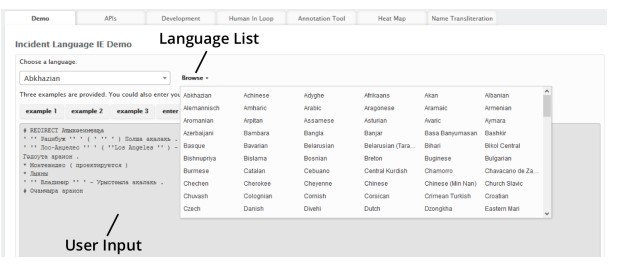
\includegraphics[width=1\textwidth]{figures/5satu.JPG}}
\caption{interface uji}
\label{gambarPFS2}
\end{figure}

\begin{figure}[ht]
\centerline{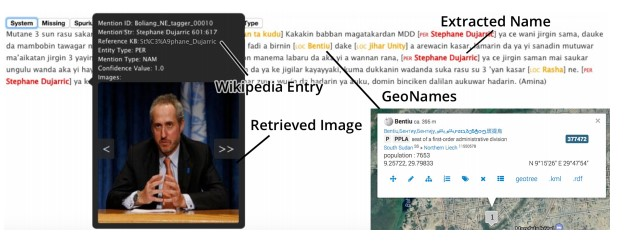
\includegraphics[width=1\textwidth]{figures/5dua.JPG}}
\caption{output}
\label{gambarPFS3}
\end{figure}

Gambar 1 menunjukkan antarmuka uji, di mana seorang pengguna dapat memilih salah satu dari 282 bahasa, masukkan teks atau pilih dokumen contoh, dan jalankan sistem. Gambar 2 menunjukkan contoh output. Sebagai tambahan ke ekstraksi entitas dan menghubungkan hasil, kami juga menampilkan 5 gambar teratas untuk setiap entitas yang diambil dari Google Image Search11. Lewat sini bahkan ketika seorang pengguna tidak dapat membaca dokumen dalam sumber rendah bahasa, dia akan mendapatkan tingkat tinggi ringkasan entitas yang terlibat dalam dokumen

memungkinkan untuk dapat melibatkan interface di mana pengguna dapat melihat satu dari banyak bahasa , teks atau pilihan documen , dan dapat di jalankan. dan di dalamnya terdapat output sebagai tambahan ke esktraksi entitas dan menghubungan hasilnya . yang berbentuk bahasa document dalam sumber yang rendah bahasa.\cite{zhangelisa}.

\subsection{membuat aplikasi dengan flask Swagger }
Swagger UI bekerja cukup baik ketika datang untuk menggambarkan dan memvisualisasikan layanan web RESTful. Menghasilkan halaman web kecil yang mendokumentasikan API dan memungkinkan Anda membuat pertanyaan pengujian menggunakan JavaScript (Karzyński, 2016). Keswaggeran didasarkan pada YAML atau JSON, dan merupakan salah satu yang paling populer. The Spesifikasi kompatibel dengan JSON Schema. Muncul dengan alat sumber terbuka untuk menghasilkan dokumentasi dan mensimulasikan server untuk diuji. Namun, antarmuka penggunanya Sepertinya ada banyak ruang untuk perbaikan. Baik klien dan server dihasilkan dan mereka mendokumentasikan secara bersamaan, sehingga mereka diperbarui pada saat yang bersamaan. Pengkodean server terkait erat dengan dokumentasinya, yang memungkinkannya dihasilkan cara yang sangat terintegrasi. Spesifikasi dibuat dari bawah ke atas\cite{ortegacatalogo}.

\subsection{Membuat Aplikasi dengan Flask Swagger}
Dokumentasi Swagger API dibuat secara otomatis dan tersedia di root API Anda tetapi Anda perlu memberikan beberapa detail, Dekorator ini memungkinkan Anda menentukan beberapa detail tentang API Anda, kemudian dapat digunakan dalam deklarasi API Swagger. Dekorator ini berfungsi seperti dekorator Flask-Restful dengan perbedaan yang mendokumentasikan metode. Parameter optionnal memungkinkan Anda untuk menentukan apakah objek dikembalikan sebagai daftar. Anda dapat memberikan dokumentasi kelas-luas dengan menggunakan parameter dokumen Api.route () ‘s’. Ini menerima atribut / sintaks yang sama dari dekorator Api.doc ()\cite{de2017api}.

\subsection{Membuat Aplikasi dengan Flask Swagger}
Flasgger adalah ekstensi Flask untuk membantu pembuatan API Flask dengan dokumentasi dan live playground yang didukung oleh SwaggerUI. Anda dapat menentukan struktur API menggunakan file YAML dan Flasgger membuat semua spesifikasi untuk Anda dan Anda dapat menggunakan skema yang sama untuk memvalidasi data.


\subsection{Membuat Aplikasi dengan Flask Swagger}
Merancang API untuk Layanan ACT dilakukan menggunakan editor Swagger (swagger.io).
Kami merancang lima API untuk memanfaatkan GFE DB: hla, gfe, ars, urutan, dan bertindak. Kita
mendefinisikan parameter dan tanggapan untuk setiap panggilan API dalam kesombongan YAML
spesifikasi. Kami menghasilkan server Python Flask menggunakan file spesifikasi Swagger
dan alat pembuat kode Sombong. Kode server yang dihasilkan telah dimodifikasi untuk diimpor
modul python yang berisi fungsi utama untuk setiap API. Fungsi masing-masing
API dimungkinkan melalui query nol yang mencari GFE DB \cite{halagan2017bioinformatics}

\subsection{Flask Swagger}
Flask-RESTPlus adalah ekstensi untuk Flask yang menambahkan dukungan untuk membangun REST API dengan cepat. Flask-RESTPlus mendorong praktik terbaik dengan penyetelan minimal. Jika Anda terbiasa dengan Flask, Flask-RESTPlus harus mudah diambil. Ini menyediakan koleksi dekorator dan alat untuk mendeskripsikan API Anda dan mengekspos dokumentasi dengan benar (menggunakan Swagger)\cite{buhler2017design}.

\subsection{Membuat Aplikasi dengan Flask Swagger}
Layanan dmon-controller pada dasarnya adalah layanan yang digunakan oleh semua komponen lain untuk berkomunikasi. Ini sebenarnya adalah titik integrasi utama dengan sisa solusi DICE. Secara khusus, ini akan digunakan oleh semua komponen DICE yang membutuhkan data pemantauan. REST API dibagi menjadi dua bagian utama: API Manajemen Pemantauan dan API Kueri Pemantauan \cite{pop2016monitoring}.

\section{Membuat Aplikasi Sederhana Dengan Python Flask + Swagger}

\subsection{Memasang Python}
Apabila komputer kita belum memiliki Python, kita hasrus pasang terlebih dahulu. Apabila, OS komputer/laptop kita tidak memiliki package dari Python, silahkan download di website resmi Python (Recomended Python 3). Jika pengguna OS Windows dengan SWL atau Cygwin,

Untuk memastikan Python telah terpasang dengan baik pada system (Saya menggunakan Windows), buka CMD dan ketikkan python,  Berikut pesan yang seharusnya muncul:

\begin{figure}[ht]
\centerline{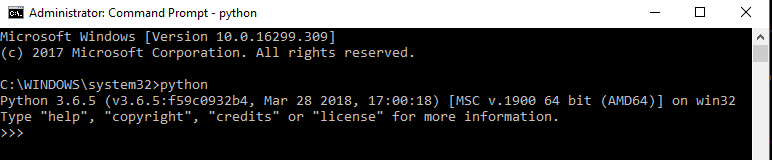
\includegraphics[width=1\textwidth]{figures/5Python.PNG}}
\caption{Python Running}
\label{gambar}
\end{figure}

\subsection{Memasang Flask}
Berikutnya ialah memasang microframework Flask. Tapi, sebelum itu, kami ingin memberitahu kepada anda tentang best practice ketika memasang package Python pada komputer anda.

Dalam Python, package seperti Flask tersedia di repositori publik dimana pengguna dapat mengunduh dan memasangnya. Repositori package resmi Python bernama Python Package Index (PyPI). Ketika menginstall sebuah package dari PyPI akan berjalan cukup mudah karena Python memiliki sebuah tool bernama pip yang dapat melakukan proses pemasangan dengan sendirinya. ntuk memasang package gunakan perintah pip :

\begin{verbatim}
 pip install <package-name>
\end{verbatim}

Python menggunakan konsep virtual environments yang merupakan hasil salinan secara keseluruhan dari interpreter Python. Ketika kita memasang sebuah package di sebuah virtual environment ini maka Python yang berada di sistem utama tidak akan terpengaruh. Virtual environment juga memiliki keuntungan dimana mereka dimiliki oleh user sehingga tidak memerlukan akun administrator.

Mari kita mulai dengan membuat sebuah direktori dimana project kita akan disimpan. Kami akan menamainya microblog karena ini ialah nama aplikasinya:

\begin{verbatim}
C:\WINDOWS\system32>cd/

C:\>mkdir microblog

C:\>cd microblog
\end{verbatim}

Jika menggunakan Python 3, virtual environment sudah ada secara otomatis sehingga bisa langsung dibuat dengan perintah:

\begin{verbatim}
C:\microblog>python -m venv venv
\end{verbatim}

Perintah tersebut mengartikan bahwa kita memerintahkan agar Python menjalankan package venv untuk membuatkan sebuah virtual environment bernama venv. venv pertama di perintah tersebut merupakan nama package-nya sedangkan venv yang kedua merupakan nama direktori untuk menyimpan salinan interpreter Python.

Apabila kita menggunanka Python versi dibawah 3.4 maka vnv masih belum menjadi package bawaan sehingga harus dipasang terlebih dahulu. Untuk versi Python-python tersebut, pasang aplikasi pihak ketika bernama virtualenv sebelum membuat virtual environment yang baru. Setelah virtualenv terpasang pada komputer maka kita dapat membuat sebuah virtual environment dengan perintah:

\begin{verbatim}
C:\microblog>virtualenv venv
\end{verbatim}

Sekarang kita seharusnya sudah memiliki virtual environment pada komputer kita. Selanjutnya, kita perintahkan kepada sistem untuk menggunakan virtual environment untuk mengaktifkannya dengan perintah:

\begin{verbatim}
C:\microblog>venv\Scripts\activate

\end{verbatim}

Sekarang setelah kita memiliki virtual environment dan menjalankannya pad sistem, selanjutnya kita tambahkan microframework Flask untuk membuat web service di dalamnya.

\begin{verbatim}
(venv) C:\microblog>pip install Flask
\end{verbatim}

Pada kasus ini kita ingin membuat aplikasi microblogging dengan memiliki sebauh heading yang menyambut visitor dalam website yang telah kita bangun. Untuk itu kita akan mengabaikan fakta bahwa aplikasi ini belum memiliki konsep user karena baru akan kita buat . Untuk mengemulasi seorang user, penulis akan menggunakan dictionary Python sebagai berikut:

\begin{verbatim}
user = {'username': 'Miguel'}
\end{verbatim}

Proses pembuatan user tersebut dikenal juga dengan istilah mocking yang memungkinkan kita untuk fokus menyelesaikan salah satu bagian aplikasi dan mengabaikan bagian yang belum selesai. Dalam kasus ini kita ingin menyelesaikan tampilan web tanpa perlu memikirkan bagaimana sistem manajemen user-nya dan bisa terus bekerja.




\section{konfigurasi Python Flask + Swagger}
Untuk mengunduh dan memulai aplikasi demo, berikan perintah berikut. Pertama-tama, klon kode aplikasi ke direktori mana pun di disk Anda:
\begin{verbatim}
$ cd /path/to/my/workspace/
$ git clone https://github.com/postrational/rest_api_demo
$ cd rest_api_demo
\end{verbatim}
Buat lingkungan virtual Python dalam direktori bernama venv, aktifkan virtualenv dan pasang dependensi yang diperlukan menggunakan pip:
\begin{verbatim}
$ virtualenv -p `which python3` venv
$ source venv/bin/activate
(venv) $ pip install -r requirements.txt
\end{verbatim}
Sekarang mari siapkan aplikasi untuk pengembangan dan mulai:
\begin{verbatim}
(venv) $ python setup.py develop
(venv) $ python rest_api_demo/app.py
\end{verbatim}
\cite{de2017api}

\subsection{Flask Swagger melalui API}
Saat anda mengakses API melalui UI web Swagger. Hal ini karena tidak mungkin untuk mengatur header otorisasi yang dienkode base64 dari UI angkuh. Bagi mereka yang bertanya-tanya "apa yang angkuh", saya akan mendefinisikan Swagger sebagai alat untuk proyek berbasis API yang menciptakan UI web yang bagus untuk melakukan uji langsung API dan juga mengekspor skema API yang dapat digunakan untuk memahami Definisi API.

\subsection{Flask Swagger dengan Restful}
Untuk pengguanaan swagger memerlukan waktu yang lama begitu juga saat menggunakan \verb|Flask-RESTful| , tetapi dalam kebutuhan dokumen yang di perlukan swagger maka muncul perintah untuk beralih ke \verb|Flask-RESTful|. Ini didasarkan pada \verb|Flask-RESTful|, jadi untuk bermigrasi hanya diperlukan dengan cara mengubah impor dari \verb|flask_restful|  impor ke \verb|Flask_RESTful| impor Selain dokumentasi swagger, dari situlah akan menambah ruang nama.


\section{Kesimpulan}
dengan dibuatnya resume ini kita dapat mengetahui secara teori tentang pembuatan aplikasi menggunakan bahasa pemrograman pyton yaitu flask + swagger . 
memungkinkan untuk melibatkan interface di mana pengguna dapat melihat satu dari banyak bahasa , teks atau pilihan documen , dan dapat di jalankan. dan di dalamnya terdapat output sebagai tambahan ke esktraksi entitas dan menghubungan hasilnya . yang berbentuk bahasa document dalam sumber yang rendah bahasa dan adapun subnya seperti di bawah ini:

\begin{enumerate}
\item mengetahui apa itu flask swagger
\item mengetahui cara pembuatan aplikasi menggunakan flask swagger
\item mengetahui fungsi dari flask swagger itu sendiri
\end{enumerate}	
cukup sekian yang dapat kami sampaikan semoga resume ini dapat bermanfaat  bagi pembaca maupun penulis .mohon maaf jika masih banyak kesalahan dalam hal penulisan maupun dalam hal penyampaian materi flask ini, kami harapkan kritik dan saran supaya dapat membuat resume menjadi lebh baik lagi untuk kedepanya kami ucapkan trimakasih banyak





% contoh aplikasi web service
% web service
% protokol
% port

% HTTP
% URL
% POST
% GET



\bibliographystyle{IEEEtran}.
\bibliography{references}.

\printindex

\end{document}
